\documentclass[10pt,english,a4paper]{article}
\usepackage[T1]{url}
\usepackage[utf8]{inputenc}
\usepackage{graphicx, varioref, babel, fancyvrb, listings, amsmath,amsthm, amssymb, enumerate}
\usepackage{listings}
\usepackage{mathtools}
\usepackage{csquotes}
\usepackage{tikz}
\usepackage{tikz-cd}
\usepackage{xcolor}

% mathbf vectors
\def\a{\boldsymbol{a}}
\def\b{\boldsymbol{b}}
\def\c{\boldsymbol{c}}
\def\dv{\boldsymbol{d}} % OBS
\def\e{\boldsymbol{e}}
\def\f{\boldsymbol{f}}
\def\g{\boldsymbol{g}}
\def\h{\boldsymbol{h}}
\def\i{\boldsymbol{i}}
\def\j{\boldsymbol{j}}
\def\k{\boldsymbol{k}}
\def\l{\boldsymbol{l}}
\def\m{\boldsymbol{m}}
\def\n{\boldsymbol{n}}
\def\ov{\boldsymbol{o}} % OBS -> compilation error with 'ø'
\def\p{\boldsymbol{p}}
\def\q{\boldsymbol{q}}
\def\rv{\boldsymbol{r}} % OBS
\def\s{\boldsymbol{s}}
\def\t{\boldsymbol{t}}
\def\u{\boldsymbol{u}}
\def\v{\boldsymbol{v}}
\def\w{\boldsymbol{w}}
\def\x{\boldsymbol{x}}
\def\y{\boldsymbol{y}}
\def\z{\boldsymbol{z}}

% Matrices
\def\A{\mathbf{A}}
\def\B{\mathbf{B}}
\def\Cm{\mathbf{C}} % OBS
\def\D{\mathbf{D}}
\def\E{\mathbf{E}}
\def\F{\mathbf{F}}
\def\G{\mathbf{G}}
\def\H{\mathbf{H}}
\def\I{\mathbf{I}}
\def\J{\mathbf{J}}
\def\K{\mathbf{K}}
\def\L{\mathbf{L}}
\def\M{\mathbf{M}}
\def\Nm{\mathbf{N}} % OBS
\def\Ov{\mathbf{O}} % OBS -> compilation error with 'Ø'
\def\P{\mathbf{P}}
\def\Qm{\mathbf{Q}} % OBS
\def\Rm{\mathbf{R}} % OBS
\def\S{\mathbf{S}}
\def\T{\mathbf{T}}
\def\U{\mathbf{U}}
\def\V{\mathbf{V}}
\def\W{\mathbf{W}}
\def\X{\mathbf{X}}
\def\Y{\mathbf{Y}}
\def\Zm{\mathbf{Z}} % OBS

% Script letters
\newcommand{\As}{\mathcal{A}}
\newcommand{\Bs}{\mathcal{B}}
\newcommand{\Cs}{\mathcal{C}}
\newcommand{\Ds}{\mathcal{D}}
\newcommand{\Es}{\mathcal{E}}
\newcommand{\Fs}{\mathcal{F}}
\newcommand{\Gs}{\mathcal{G}}
\newcommand{\Hs}{\mathcal{H}}
\newcommand{\Is}{\mathcal{I}}
\newcommand{\Js}{\mathcal{J}}
\newcommand{\Ks}{\mathcal{K}}
\newcommand{\Ls}{\mathcal{L}}
\newcommand{\Ms}{\mathcal{M}}
\newcommand{\Ns}{\mathcal{N}}
\newcommand{\Os}{\mathcal{O}}
\newcommand{\Ps}{\mathcal{P}}
\newcommand{\Qs}{\mathcal{Q}}
\newcommand{\Rs}{\mathcal{R}}
\newcommand{\Ss}{\mathcal{S}}
\newcommand{\Ts}{\mathcal{T}}
\newcommand{\Us}{\mathcal{U}}
\newcommand{\Vs}{\mathcal{V}}
\newcommand{\Ws}{\mathcal{W}}
\newcommand{\Xs}{\mathcal{X}}
\newcommand{\Ys}{\mathcal{Y}}
\newcommand{\Zs}{\mathcal{Z}}

% Often used number systems. 
\def\C{\mathbb{C}}
\def\Z{\mathbb{Z}}
\def\N{\mathbb{N}}
\def\Q{\mathbb{Q}}
\def\R{\mathbb{R}}

% dx
\def\d{~\text{d}}
\def\dla{~\text{d}\lambda}
\def\dmu{~\text{d}\mu}
\def\dnu{~\text{d}\nu}

% Words
\def\dim{\text{ dim}}
\def\conv{\textnormal{conv}} 
\def\card{\textnormal{card}}
\def\supp{\textnormal{supp}}
\def\rank{\textnormal{rank}}

% Arrows
\def\Uda{\Updownarrow}
\def\ua{\uparrow}
\def\ra{\rightarrow}
\def\Ra{\Rightarrow}
\def\Lra{\Longleftrightarrow}
\def\lra{\leftrightarrow}
\def\laa{\leftarrow}
\def\Laa{\Leftarrow}
\def\Da{\Downarrow}

% dots
\def\ld{\ldots}
\def\vd{\vdots}
\def\cd{\cdots}
\def\dd{\ddots}

% Braces
\def\({\left(}
\def\){\right)}



%Greek Letters
\def\eps{\epsilon}
\def\la{\lambda}
\def\La{\Lambda}
\def\om{\omega}
\def\Om{\Omega}
\def\al{\alpha}
\def\Al{\Alpha}
\def\ga{\gamma}
\def\Ga{\Gamma}

% others
\def\pa{\partial}
\def\ul{\underline}
\def\ol{\overline}
\def\ob{\overbrace}
\def\ub{\underbrace}
\def\bs{\boldsymbol}
\def\ti{\times}



%newcommand
\newcommand{\ind}[1]{\left\langle #1 \right\rangle}
\newcommand{\indi}[1]{\langle #1 \rangle}
\newcommand{\floor}[1]{\left\lfloor #1 \right\rfloor}
\newcommand{\ceil}[1]{\left\lceil #1 \right\rceil}
\newcommand{\nlist}[1][]{{#1}_1, {#1}_2, \ldots, {#1}_{n}}
\newcommand{\dlist}[2][]{{#1}_1, {#1}_2, \ldots, {#1}_{#2}}
\newcommand{\oo}[1][2]{\frac{1}{#1}}
\newcommand{\po}[1][2]{\frac{\pi}{#1}}
\newcommand{\Span}[1]{\text{span} \left\{#1\right\} }
\newcommand{\File}[1]{\fvset{fontsize=\small, frame=lines}%,
                            % numbers=left, numbersep=3pt} 
                            \VerbatimInput{#1}}

\usepackage{marginnote}

%\declaretheorem[style = remark, sibling = lemma, qed = $\maltese$, name = "]{thm}

\makeatletter
\def\moverlay{\mathpalette\mov@rlay}
\def\mov@rlay#1#2{\leavevmode\vtop{%
   \baselineskip\z@skip \lineskiplimit-\maxdimen
   \ialign{\hfil$\m@th#1##$\hfil\cr#2\crcr}}}
\newcommand{\charfusion}[3][\mathord]{
    #1{\ifx#1\mathop\vphantom{#2}\fi
        \mathpalette\mov@rlay{#2\cr#3}
      }
    \ifx#1\mathop\expandafter\displaylimits\fi}
\makeatother

\newcommand{\cupdot}{\charfusion[\mathbin]{\cup}{\cdot}}
\newcommand{\bigcupdot}{\charfusion[\mathop]{\bigcup}{\cdot}}



\theoremstyle{definition}
\newtheorem*{definition}{Definition}
\newtheorem*{theorem}{Theorem}
\newtheorem*{lemma}{Lemma}
\newtheorem*{corollary}{Corollary}
\newtheorem*{proposition}{Proposition}
\newtheorem*{observation}{Observation}
\newtheorem*{example}{Example}
\newtheorem*{exercise}{Exercise}
\newtheorem*{note}{Note}
\newtheorem*{notation}{Notation}
\newtheorem*{remark}{Remark}

\let\emph\relax % there's no \RedeclareTextFontCommand
\DeclareTextFontCommand{\emph}{\bfseries}
%\begin{figure}
%    \centering
%    \includegraphics[width=0.8\linewidth]{nameOfFile}
%    \caption{}
%\end{figure}

\def\Psfin{\mathcal{P}_{\textnormal{fin}}}
\def\Fbb{\mathbb{F}}
\def\Tbb{\mathbb{T}}
\def\Ff{\mathcal{F}}
\def\Kf{\mathcal{K}}
\def\ex{\textnormal{ex}\,}
\def\co{\textnormal{co}\,}
\def\whAs{\widehat{\As}}
\def\tAs{\widetilde{\As}}
\def\tBs{\widetilde{\Bs}}
\def\Assa{\As_{\text{sa}}}
\def\sa{\text{sa}}
\def\tvphi{\tilde{\varphi}}
\def\Hpi{H_{\pi}}
\def\dA{\dot{A}}
\def\dB{\dot{B}}
\def\Hpi{H_{\pi}}
\def\eal{e_{\alpha}}
\def\ebe{e_{\beta}}
\def\ega{e_{\gamma}}
\def\deal{\dot{e}_{\alpha}}
\def\debe{\dot{e}_{\beta}}
\def\dega{\dot{e}_{\gamma}}
\def\dA{\dot{A}}
\def\dB{\dot{B}}

\def\pivp{\pi_{\vphi}}
\def\Hvp{H_{\vphi}}
\def\xivp{\xi_{\vphi}}
\def\etavp{\eta_{\vphi}}

\def\piess{\pi^{\text{ess}}}
\DeclareMathOperator{\Rep}{Rep}
\DeclareMathOperator{\Proj}{Proj}
\DeclareMathOperator{\Id}{Id}
\DeclareMathOperator{\Sp}{sp}
\DeclareMathOperator{\Tr}{Tr}
\DeclareMathOperator{\diag}{diag}
\DeclareMathOperator{\vN}{v.N}
\def\vphi{\varphi}
\def\top{\tilde{\oplus}}

%%% Colours %%%
\newcommand*{\BLUE}[1]{{\color{blue}#1}}
\newcommand*{\RED}[1]{{\color{red}#1}}
\newcommand*{\GREEN}[1]{{\color{green}#1}}


\title{Notes MAT4360}
%\author{Vegard Antun \\MAT 4450 }

\begin{document}
\maketitle

\section{Compact operators}
We will always assume that the scalar field is $\C$. By an operator we will always 
mean a linear operator. $H$ will denote a non-zero Hilbert space and 
$H_1 \coloneqq \{ \xi \in H : ||\xi||\leq 1 \}$.

Recall that an operator $T \colon H \to H$ is called \emph{compact} if 
$\{T(\xi_n)\}_{n \in \N}$ has a convergent subsequence whenever $\xi_n$ is 
a bounded sequence in $H$.

This is equivalent to requiring that $T$ maps bounded sets in $H$ into relative compact (i.e. closure is compact) sets of $H$.

\begin{itemize}
    \item Every compact operator is bounded. 
    \item Every bounded finite rank (finite-dimensional image) operator is compact.
    \item $\Ff(H) = \{ T \in \Bs(H): T \text{ has finite rank} \}$. 
    \item $\Kf(K) = \{T \in \Bs(H) : T \text{ is compact operator}\}$.
\end{itemize}
One can show that $\ol{\Ff(H)}^{||\cdot||} = \Kf(H) \subset \Bs(H)$ 
and $\Kf(H) \neq \Bs(H)$ when $H$ is infinite dimensional (Since $I_{H} \in
\Kf(H) \iff H$ is finite dimensional). 

\begin{itemize}
    \item $\Ff(H)$ and $\Ks(H)$ are both ideals in $\Bs(H)$. 
\end{itemize}
Note: by ideal in an algebra we will always mean, unless otherwise specified a two-sided ideal.
So 
\[S \in \Ff(H), T \in \Bs(H)  \implies \begin{cases} ST \in \Ff(H) \\ TS \in \Ff(H) \end{cases}\]
Moreover they are both \emph{self-adjoint} ideals (A subset $\Js \subset
\Bs(H)$ is called self-adjoint if $S \in \Js \implies S^* \in \Js$).
\begin{proposition}
\leavevmode
\begin{enumerate}[1)]
        \item $\Ff(H)$ is the least non-zero ideal of $\Bs(H)$. 
        \item $\Kf(H)$ is the least non-zero, norm-closed ideal of $\Bs(H)$. 
    \end{enumerate}
\end{proposition}
\begin{proof}
    We first observe that any finite rank $S \in \Ff(H)$ is of the form 
    \[ S(x) = \sum_{j=1}^{n} \ind{x,\eta_j}\xi_j  \quad \text{ for some }\eta_1, 
    \ldots, \eta_n,\xi_1,\ldots, \xi_n\in H, ~\xi_j \neq 0\]
    Indeed, let $\{\xi_1, \ldots, \xi_n\}$ be an orthonormal basis for $S(H)$ (image of $S$, for $S\neq 0$). Then $Sx = \sum_{j=1}^{n} \ind{Sx, \xi_j}\xi_j = \sum_{j=1}^{n}\ind{x,S^*\xi_j}\xi_j$ for all $x \in H$

\begin{itemize}
    \item 
Let now $\Js \neq \{0\}$ be an self-adjoint ideal of $\Bs(H)$. We have to show that 
$\Ff(H) \subseteq \Js$. Since $\Js$ is a subspace we see that it is enough to show that 
$\Js$ contains all operators of the form $x\mapsto \ind{x,\eta}\xi$ where $\xi
\in H\setminus\{0\}$.

We pick $T \in \Js$, $T \neq 0$. We then have $T\xi_0 = \eta_0$ for some 
$\xi_0 \in H\setminus\{0\}$, $\eta_0 \in H_1$ (normalize if needed). Let
$\xi\in H\setminus\{0\}$, $\eta \in H$. Define $A,B,S \in \Bs(H)$ by 
\[  Ax = \ind{x,\eta_0}\eta, \quad Bx = \ind{x,\xi}\xi_0, \quad \text{for all } x\in H \]
and $S = ATB$. Then $S \in \Js$ (since $\Js$ is an ideal and $T \in \Js$) and 
\[Sx = \ind{x,\xi}AT\xi_0 = \ind{x,\xi}A\eta_0 = \ind{x,\xi} \ind{\eta_0,\eta_0}\eta
= \ind{x,\xi}\eta, \quad \text{for all }x\in H\]
which shows what we wanted.

\item Assume $\Js$ is a non-zero norm-closed ideal in $\Bs(H)$. Then $\Ff(H) \subseteq \Js$
by $1)$ so $\Kf(H) =\ol{\Ff(H)}^{||\cdot||}  \subseteq \Js$ since $\Js$ is norm-closed
\end{itemize}
\end{proof}
\begin{remark}
    A $C^*$-algebra $\As$ is called \emph{simple} when $\{0\}$ and $\As$ are
the only closed ideals of $\As$. From the above proof we see that if $\Js$ is a
norm-closed ideal of $\Kf(H)$ which is non-zero then we also get
$\ol{\Ff(H)}^{||\cdot||} = \Kf(H) \subseteq \Js \subseteq \Kf(H)$, so $\Js =
\Kf(H)$.
This means that $\Kf(H)$ is simple. In particular $M_n(\C) \simeq \Kf(\C^n) =
\Bs(\C^n)$ is simple.
\end{remark}

\begin{theorem}
    The following conditions are equivalent, given $T \in \Bs(H)$.
    \begin{enumerate}[(1)]
        \item $T$ is compact.
        \item $T \lvert_{H_1} \colon (H_1, \text{rel. weak. top}) \to (H, \text{norm-top.})$ is 
        continuous.
        \item $T(H_1)$ is norm-compact in $H$. 
        \item For every net $\{\xi_{\al}\}$ in $H_1$ the net $\{T\xi_{\al}\}$ has 
              a convergent subnet.
    \end{enumerate}
\end{theorem}

Note: $(3) \iff (4)$ by the characterization of compactness with help of nets.

\begin{proof}
    Note that we need lemma 1-4 below. 
    $(1)\implies (2)$ Assume $T$ is compact. Let $\{\xi_{\al}\}$ be a net in $H_1$ which 
    converges weakly to some $\xi\in H_1$. Let $\eps > 0$ and pick 
    $S \in \Ff(H)$ such that $||S-T|| < \eps/3$. Now we have 
\[ ||T\xi_{\al} - T\xi || \leq \ub{||T\xi_{\al} - S\xi_{\al}||}_{\leq ||T-S||}
+ ||S\xi_{\al} - S\xi|| + \ub{||S\xi-T\xi||}_{\leq ||T-S||}\]
since $S$ is weak-weak continuous (cf. lemma 4) we have that $S\xi_{\al}\to S\xi$ 
weakly. But the range of $S$ is finite dimensional, so we can use lemma 1 with 
$X = \text{Range}(S)$ to deduce that $||S\xi_{\al}-S\xi||\leq \eps/3$ for all 
$\al \geq \al_0$. Then for $\al \geq \al_0$ we get 
$||T\xi_{\al} - T\xi|| \leq 2\eps/3 + \eps/3 = \eps$ which shows that 
$T\xi_{\al} \to T\xi$ in norm as desired.

$(2)\implies (3)$ This follows from lemma 2. $(3) \iff (4)$ is ok. 

$(4) \implies (1)$. Assume $(4)$ holds. 
Let $P_{\la}$ be as in lemma 3. Then $P_{\la}T \in \Ff(H)$ for all $\la$. 
We want to show that $P_{\la}T \to T$ in operator norm. Assume this is not true. 
Then there exists $\eps > 0$ such that we can find
(by eventually going to subnets) some $\xi_{\la} \in H_1$ such that $||(P_{\la}T-T)\xi_{\la}||\geq \eps$.

Using $(4)$ we can now assume that $\{T\xi_{\la}\}$ converges to some $\eta \in H$
(again by going to subnets if necessary). Then using lemma 3 we get 
\begin{align*}
    ||(I-P_{\la})T\xi_{\la}|| &\leq 
    ||(I-P_{\la})(T\xi_{\la}-\eta)|| + ||(I-P_{\la})\eta|| \\
    &\leq \ub{||I-P_{\la}||}_{\leq 1} ||T\xi_{\la} -\eta|| +
    ||\eta-P_{\la}\eta|| \to 0
\end{align*}
We have  a contradiction. 


 
\end{proof}


To prove this we will need some lemmas:
\begin{lemma}[1]
    Assume $X$ is a finite dimensional vector space. Then there exists only one 
    topology $\tau$ (up to homeomorphism) such that $(X,\tau)$ is a locally 
    convex Hausdorff topological vector space.
\end{lemma}

\begin{proof}
    Let $\Bs = \{x_1,\ldots, x_n\}$ be a basis for $X$. We can then define a 
norm on $X$ by $||x|| = ||[x]_{\Bs}||$ where $[x]_{\Bs}$ is the coordinate
representation of $x$ in $\Bs$ and $||\cdot ||$ is the euclidean norm. 

$(X, ||\cdot ||)$ is a locally convex Hausdorff topological vector space with 
respect to the norm topology, which is homeomorphic to ($\C^n$, euclidean top.) (via the map $x\mapsto [x]_{\Bs}$). 

Let now $\tau$ be any topology on $X$ such that $(X,\tau)$ is a locally 
convex Hausdorff topological vector space. We will show that $(X,\tau)$
is homeomorphic to ($C^n$,  Euclidian top.).

We will first show that there exits $\rho_1,\ldots, \rho_n \in (X,\tau)^{*}$
(dual space) such that $\rho_j(x_i) = \delta_{ij}$ (Kronecker delta) for all 
$i,j \in \{1,\ldots, n\}$. Define $S\colon (X,\tau)^* \to C^n$
by $S(\rho) = [\rho(x_1),\ldots, \rho(x_n)]$. It is clear that $S$ is linear,
moreover it is surjective:

Assume this is not true. Then $M \coloneqq \text{Range}(S)$ is a subspace of $\C^n$
different from $\C^n$, so $M^{\perp}\neq \{0\}$, so we can pick some vector 
$c \in \C^n \setminus \{0\}$ such that $c\perp M$ i.e. $\rho(x_1)\bar{c}_1 + 
\ldots + \rho(x_n)\bar{c}_n = 0$ for all $\rho \in (X, \tau)^*$ i.e.
$\rho(\bar{c}_1x_1 + \ldots + \bar{c}_n x_n) =  0 $ for all $\rho \in (X,\tau)^*$.
By a corollary of the Hahn-Banach separation theorems we get that 
$\bar{c}_1 x_1 + \ldots + \bar{c}_n x_n  = 0$ (since we can separate points).
But $x_1,\ldots, x_n$ are basis elements (linear independent), so 
$c_1 = \ldots = c_n = 0$, i.e. $c=0$.

This mean that we can find $\rho_1,\ldots, \rho_n \in (X,\tau)^*$
such that $S(\rho_j) = e_j $ (standard basis vector in $C^n$).
That is $\rho_{j}(x_i) =\delta_{ij}$ for all $i,j \in \{1,\ldots,n\}$.

Now we can define $T\colon X \to \C^n$ by $T(x) = (\rho_1 (x),\ldots,
\rho_n(x))$ , which is clearly linear and continuous with respect to $\tau$.  For $x =
\sum_{i=1}^{n}\la_i x_i \in X$ we have $\rho_{j}(x) =\sum_{i}^{n}
\la_{j}\rho_j(x_i) = \la_j$. Thus $T(x) = (\la_1,\ldots,\la_n) = [x]_{\Bs}$ for
all $x$, so $T$ is the coordinate map with respect to $\Bs$, which is an
isomorphism with $T^{-1}(\la_1,\ldots,\la_n) = \la_1x_1 + \ldots, \la_nx_n$. We
see that $T^{-1}$ is continuous because the vector space operations are
continuous with respect to $\tau$.
\end{proof}


\begin{lemma}[2]
    $H_1$ is weak-compact. 
\end{lemma}

\begin{proof}
    We know the map $\eta  \to \vphi_{\eta}$ from $H $ into $H^*$ is bijective 
and \emph{isometric}, where $\varphi_{\eta}(\xi) = \ind{\xi,\eta})$ for $\xi \in H$
(conjugate linear). Moreover we have that if $\{\xi_{\al}\}$ is a net in $H$
and $\xi \in H$, then $\{\xi_{\al}\}$ converges weakly to $\xi$.
 \begin{align*}
     \iff& \varphi_{\eta}(\xi_{\al}) \to \varphi_{\eta}(\xi) ~\forall \eta \in H \\
     \iff& \ind{\xi_{\al},\eta} \to \ind{\xi,\eta} ~\forall \eta \in H \\
     \underset{\text{by conjugation}}{\iff}& \ind{\eta, \xi_{\al}} \to \ind{\eta, \xi} ~\forall \eta \in H \\
\iff&\vphi_{\xi_{\al}}(\eta) \to \varphi_{\xi}(\eta) ~\forall\eta\in H
 \end{align*}
$\iff$ $\{\vphi_{\xi_{\al}}\}$ converges to $\vphi_{\xi}$ in the weak$^*$-topology
of $H^*$.

It follows that $\eta \overset{\varphi}{\to} \varphi_{\eta}$ is a
homeomorphism of $(H,\text{weak top})$ onto $(H^*, \text{weak}^*\text{ top.})$.
Now Alaogu's theorem gives that $(H^*)_1$ is weak$^*$-compact. 
Hence we get that $H_1 = \underset{\text{cont.}}{\varphi^{-1}}(\underset{\text{weak}^*\text{ compact}}{(H^*)_1})$.
\end{proof}

\begin{lemma}[3]
    There exists a net $\{P_{\la}\}$ of projections with finite rank such that 
    $\lim_{\la} ||P_{\la} \xi - \xi|| = 0$ i.e. $\lim_{\la} P_{\la} = I_{H}$ 
    in the strong operator topology. 
\end{lemma}
\begin{proof}
   Let $\{e_j\}_{j\in \N}$ be an orthonormal basis for $H$. We have seen that for $x \in H_1$, 
we have $x = \sum_{j \in J} \ind{x,e_j}e_j$ means that the net $\{ \sum_{j\in F} \ind{x,e_j}e_j \}_{F\in\Psfin(J)}$ for any $\la \in \Psfin(J)$, we have that the orthogonal projection
$P_{\la}$ from $H$ onto  $\Span{e_j:j\in \la}$ is given by 
\[ P_{\la}(x) = \sum_{j\in\la} \ind{x,e_j}e_j. \]
So we see that $P_{\la}(x) \to x$ in norm for all $x \in H$, as we wanted to show.
\end{proof}

\begin{example}
    Assume that $T \in \Bs(H)$ is diagonalizable in the sense that there exists 
an orthonormal basis $\{e_j\}_{j \in J}$ for $H$ and $\{\la_j\}_{j\in J} \in
\ell^{\infty}(J)$ such that $T(e_j) = \la_je_j$ for all $j\in J$. Hence such that 
\[ T(x) = \sum_{j \in J} \la_{j}\ind{x, e_j}e_j ~\forall x \in H \]
Then we have that $T \in \Kf(H)\iff \{\la_j\}_{j\in J} \in C_{0}(J)$ 
\begin{itemize}
    \item[*] $\underset{\text{by def.}}{\iff}$ For every $\eps >0$, there exists
    a finite subset $K_{\eps}$ of $J$ such that $|\la_j|<\eps$ for all $j\in
    J\setminus K_{\eps}$.

    \item[**] $\underset{\text{easy}}{\iff}$For $\eps >0$, the set $J_{\eps}\coloneqq \{ J \in J : |\la_j| \geq \eps\}$
    is finite
\end{itemize}
\begin{proof}
   Assume $*$ holds. For every nonempty $F \in \Psfin(J)$, we define $T_F \in \Ff(H)$
by $T_{F}(x) = \sum_{j \in F}\la_j\ind{x,e_j}e_j$. Then $\{T_F\}$ converges to 
$T$ in norm: 

Let $\eps>0$. For any $F \in \Psfin(J)$
such that $K_{\eps} \subset F$ we have 
\begin{align*}
||(T-T_F)x||^2 &= ||\sum_{j\in J\setminus F}\la_j\ind{x,e_j}e_j||^2 
= \sum_{j\in J\setminus F} |\la_j|^2 |\ind{x,e_j}|^2 \\
&\leq \sum_{j\in J\setminus K_{\eps}} |\la_j|^2 |\ind{x,e_j}|^2 
< \eps^2 \sum_{j \in J\setminus K_{\eps}}|\ind{x,e_j}|^2 \underset{\text{Bessel}}{\leq}\eps^2 ||x||^2
\end{align*}
Se we get that $||T-T_F|| < \eps$, showing that $T_F \to T$ in operator-norm. 

Conversely, assume that $(*)$ does not hold i.e. there exists $\eps>0$ such that 
$J_{\eps}$ is infinite. Then we can pick $\{j_k\}_{k\in \N} \subseteq J_{\eps}$
with $j_k \neq j_{k'}$ for $k\neq k'$. Since $\sum_{k=1}^{\infty}
|\ind{x,e_{j_k}}|^2 \leq ||x||^2 <\infty$, we have that $\ind{x,e_{j_k}} \to 0$
as $k\to \infty$ so $\{e_{j_k}\}_{k\in \N}$ converges to 0 weakly (we can flip the order). 
Now $||Te_{j_k}|| = ||\la_{j_k}|| \geq \eps$ for all $k \in \N$ ($H_1$ is weak-compact). Hence $\{Te_{j_k}\}$
does not converge to $0 = T(0)$, so $T\lvert_{H_1}$ is not weak-norm continuous. 
Using the previous theorem, this shows that $T$ is not compact. (We will show later that 
every compact normal operator is diagonalizable).
\end{proof}
\end{example}


\begin{lemma}[4]
    Let $T \in \Bs(H)$. Then $T \colon (H ,\text{ weak top.}) \to (H, \text{ weak top.})$
is continuous. Moreover $T(H_1)$ is normed closed.
\end{lemma}
\begin{proof}
    Assume $\{\xi_{\al}\}$ is a net in $H$ converging weakly to $\xi \in H$.
    Then
    \begin{align*}
        \ind{T(\xi_{\al}),\eta} &= \ind{\xi_{\al}, T^*\eta} \to
        \ind{\xi,T^*\eta}= \ind{T\xi,\eta} ~~\text{ all } \eta\in H 
    \end{align*}
    Thus $T\xi_{\al} \to T\xi$ weakly, which shows the first assertion.

    Using lemma 2 we can then get that $H_1$ is compact in the weak topology. 
    In fact $T(H_1)$ is weakly closed. Hence $T(H_1)$ is normed closed. 
\marginnote{$\ol{S}^{||\cdot||} \subseteq \ol{S}^{WOT}$} 
\end{proof}


\section{About non-unital $C^*$-algebras}
Let $\As$ be a Banach $*$-algebra. If $\As$ is non-unital, as in before, we can 
\textquote{adjoin a unit to $\As$} by setting $\tilde{A} = \As\times\C$ equipped 
with the operations 
\begin{align*}
    (A,\la) + (B,\mu) &= (A+B, \la+\mu) \\
    c(A,\la) &= (cA,c\la), ~~c \in \C \\
    (A,\la)(B,\mu) &= (AB + \mu A + \la B, \la\mu) \\
    (A,\la)^* &= (A^*, \bar{\la})
\end{align*}
and the norm $||(A,\la)|| = ||A|| + |\la|$.
Then $\tilde{A}$ is a unital $*$-algebra with $I = (0,1)$ and 
$A\mapsto (A,0)$ is a \ul{isometric} $*$-homomorphism form $\As$ into $\tilde{\As}$ 
and write $\tilde{A} = (A + \la I, A \in \As, \la \in \C)$.

Assume now that $\As$ is a non-unital $C^*$-algebra. Then we may form $\tilde{\As}$
as above, but the problem is that the above norm does not satisfy the $C^*$-equality
in general. Consider e.g. $\As = C_{0}(\R) = \{f \colon \R \to \C : f \text{
cont. } \lim_{t\to\pm\infty}f(t) =0\}$ as a $C^*$-subalgebra of $C_b(\R)$ with
$||\cdot||_{\infty}$.
Then one can find $f \in \As$ such that $||(f,1)^*(f,1)|| \neq ||(f,1)||^2$ (Exercise!)
Argue also that $\As$ is non-unital.

\begin{figure}[htbp]
    \centering
    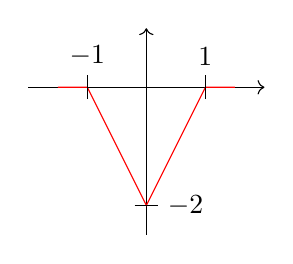
\begin{tikzpicture}[scale=0.75]
        \draw[->] (-2,0) -- (2,0);
        \draw[->] (0,-2.5) -- (0,1);
        \draw[red] (-1.5,0) -- (-1,0) --(0,-2) -- (1,0) -- (1.5,0);
        \draw (-1,-0.2) -- (-1,0.2) node[above]{$-1$};
        \draw (1,-0.2) -- (1,0.2) node[above]{$1$};
        \draw (-0.2, -2) -- (0.2, -2) node[right]{$-2$};
    \end{tikzpicture}
    \caption{ One possible function $f \in \C_0(\R) = \As$ which does not satisfy the $C^*$-equality in $\tAs$} 
    %\label{}
\end{figure}


\subsection{Adjoining a unit}


To adjoin a unit to a non-unital $C^*$-algebra, we will first introduce the multiplier 
algebra. Let $\As$ be a non-zero $C^*$-algebra. We can form the Banach algebra 
$\Bs(\As)$ of bounded operators on $\As$ with the operator norm. However, in 
general this norm does not satisfy the $C^*$-equality. We don't even have a 
$*$-operation! 

\begin{definition}
    
Let us write $\ind{A,B} = A^*B$ for $A,B \in \As$. Then let us
say that an operator 
$ T \colon \As \to \As$ is \emph{adjointable}
if there exist an operator $S\colon \As \to \As$ such that $\ind{A,T(B)}= \ind{S(A), B}$
for all $A,B \in \As$. That is $A^*T(B) = S(A)^*B$.
\end{definition}


\begin{note}
    $S$ is then necessarily unique and $T$ is bounded.
\end{note}
\begin{proof}
    Assume that $S'$ has the same property as $S$. Then $A^* T(B) = S'(A)^*B = S(A)^*B$
for all $A,B \in \As$. That is $(S(A)-S'(A))^*= 0$ for all $A,B \in \As$. In particular 
$(S(A) -S'(A))^*(S(A)-S'(A)) =0$ which implies that $||S(A)-S'(A)||^2 = 0$ i.e.
$S(A)=S'(A)$ for all $A \in \As$, so $S = S'$.

Moreover $T$ is bounded. 
Assume that $B_n \to B$, $T(B_n) \to C$ in $\As$. Then 
\begin{align*}
A^*(T(B)-C) &=
A^* (T(B)-T(B_n)) + A^*(T(B_n)-C) \\
&= A^*(T(B-B_n)) + A^*(T(B_n)-C) \\ &= S(A)^*(B-B_n) + A^*(T(B_n)-C) \to 0
\end{align*}
Hence $A^*T(B) = A^*C $ for all $A \in \As$. Thus $T(B) = C$ (same trick as above).
\end{proof}

We call $S$ the adjoint of $T$ and denote it by $T^*$. We say that 
\[M(\As) = \{\text{all adjointable operators on }\As\} \subseteq \Bs(\As)\].

\begin{example}
    Let $A \in \As$. Define the operator $L_A \colon \As\to\As$ by $L_A(B) = AB$
for all $B \in \As$. Then $L_A$ is adjointable with $(L_{A})^* = L_{A^*}$. 
Indeed, 
\[L_{A^*}(B)^*C  = (A^*B)^*C = B^*AC = B^*L_{A}(C)\quad \text{for all } B, C \in \As.\]
So we get a map $L\colon \As \to M(\As)$ sending $A \mapsto L_{A}$. 
\end{example}

\begin{proposition}
    $M(\As)$ is a closed subalgebra of $\Bs(\As)$, which is a unital $C^*$-algebra 
with respect to the involution $T \mapsto T^*$ and the operator norm on $\Bs(\As)$
($M(\As)$ is called the \emph{Multiplier algebra of $\As$})
\end{proposition}
\begin{proof}
$A^*T^*(B) = (T^*(B)^* A)^* = (B^*T(A))^* = T(A)^*B^*$ for all $A,B\in \As$.
Similarly if $S,T \in M(\As)$, we get that $(S+T)^* = S^* + T^*$ and 
$(ST)^* = T^*S^*$ and $(\la S)^* = \ol{\la}S^*$ for all $\la \in \C$.
In other words $M(\As)$ is a $*$-algebra and a subalgebra of $\Bs(\As)$.
Let $T \in M(\As)$. Then $T^* \in M(\As)$ and $(T^*)^* = T$.

\marginnote{Cauchy sequence}
We now show that $M(\As)$ is  closed in operator norm in $\Bs(\As)$:
Let $\{T_n\}_{n\in \N} \subseteq M(\As)$ be such that $T_n \to T$ in the operator norm. 
We have to show that $T$ is adjointable. $\{T_n\}$ is Cauchy in $\Bs(\As)$. We will
soon see that the $*$-operation is isometric in $M(\As)$, hence we can use 
that $\{T_{n}^{*}\}$ is also Cauchy in $\Bs(\As)$, which is complete. Thus 
$T_{n}^* \to S$ for some $S \in \Bs(\As)$. This gives that 
\marginnote{$*$-operation isometric}
\[S(A)^*B 
=\lim_{n\to\infty} T_{n}^{*}(A)^*B 
=\lim_{n\to\infty} A^*T_{n}(B) 
= A^*T(B)
\]
for all $A,B \in \As$. Hence $T$ is adjointable (with $T^* = S$). 
It remains to show that the $C^*$-equality holds (and the inverse is
isometric). Let $T \in \Ms(\As)$. Then 
\begin{align*}
||T^*T || = \sup \{ ||(T^*T)(A) || : A \in \As_1\}
&=  \sup \{ ||T^*(T(A))^* || : A \in \As_1\}  \\
&\geq \sup\{ ||\ub{T^*(T(A))^*A}_{T(A)^*T(A)} || : A\in \As_1 \} \\
&= \sup\{ ||T(A)||^2 : A \in \As_1 \} = ||T||^2 
\end{align*}
Thus we have $||T||^2 \leq ||T^*T|| \leq ||T^*||\,||T||$.
Hence $||T|| \leq ||T^*||$. Using this on $T*$ we get $||T^*|| \leq ||(T^*)^*|| = ||T||$.
Hence $||T|| = ||T^*||$. Trivial that $I_{\As}$ is adjointable. 

\end{proof}

\begin{proposition}
    The map $A \overset{L}{\to} L_A$ is an isometric $*$-homomorphism from 
$\As$ into $M(\As)$. Moreover $L(\As)$ is a closed ideal in $M(\As)$.
\end{proposition}

\begin{proof}
    
Have seen that $(L_A)^* = L_{A^*}$ so $L$ is $*$-preserving. It is easy to 
check that $L$ is an homomorphism. \ul{$L$ is isometric}: Let $A \in \As$.
We have $||L_A|| = \sup \{ ||AB|| : B \in \As_1  \} \leq ||A||||B|| \leq ||A||$.
If $A \neq 0$, set $B = \tfrac{1}{||A||}A^* \in \As_1$. Then 
\[
||L_A(B)|| = ||\tfrac{1}{||A||}AA^*|| = \frac{1}{||A||} ||(A^*)^*A^*|| = \frac{1}{||A||}
||A^*||^2 = ||A||
\]
which implies that $||L_A|| \geq ||A||$.

To show that $L(\As)$ is an ideal in $M(\As)$: Let $T \in M(\As)$, $A \in \As$.
\[ 
(L_{A^*}T)(B) = \ub{A^*T(B)}_{\ind{A,T(B)}} = \ub{T^*(A)^*B}_{\ind{T^*(A), B}} = L_{T^*(A)^*} (B) \quad \text{ for all }B \in \As
\]
\[\implies L_A T = L_{(A^*)^*} T = L_{T^*(A^*)^*} \in L(\As)   \]
i.e. $L(\As)$ is a right ideal. Moreover $(TL_A)^* = L_{A^*}T^* = L_{(T(A))^*}$
where the last equality follows by what we have just done. 
Taking the adjoint gives
\[ TL_A = (L_{T(A)^*})^* = L_{T(A)}  \in L(\As) \]
so $L(\As)$ is a left ideal. $L(\As)$ is closed in $M(\As)$ because $L$ is isometric 
(so $L(\As)$ is complete).
\end{proof}

Note that if $\As$ is unital with unit $I$, then $M(\As)= L(\As) \simeq \As$.
Indeed, let $T \in M(\As)$ and let $A = (T^*(I))^* \in \As$. Then 
\begin{align*}
    L_{A}(B) = \ub{(T^*(I))^*B}_{\ind{T^*(I), B}} = \ub{I^*
T(B)}_{\ind{I,T(B)}}= T(B) \quad \text{ for all } B \in \As
\end{align*}
so $T = L_{A} \in L(\As)$.

\subsection{Adjoining a unit to a non-unital $C^*$-algebra}
Let $\As$ be a $C^*$-algebra and consider a $*$-algebra $\tilde{\As}$ as 
defined previously. Define 
\[ \tilde{L}\colon \tilde{\As} \to M(\As) \]
by $\tilde{L}((A,\la)) = L_A + \la I_{\As}$ for $(A,\la) \in \As$.
One readily checks that $\tilde{L}$ is a $*$-homomorphism.


\begin{lemma}
    Assume $\As$ is non-unital. Then $\tilde{L}$ is injective. (Does not hold for unital) 
\end{lemma}
\begin{proof}
    Assume for contradiction that $\tilde{L}$ is not injective. So there exist 
$(A,\la) \in \tilde{\As}\setminus \{0,0\}$ such that $\tilde{L}(A,\la) = 0_{\As} \in M(\As)$ (recall it is a linear map)
i.e. $(L_A + \la I_{\As})(B) = AB + \la B = 0$ for all $B \in \As$.

If $\la = 0$, we get $AB = 0$ for all $B \in \As$ which implies that $A =0$,
which is a contradiction. Hence we must have $\la \neq 0$. 
Then we get that $(-\tfrac{1}{\la}A)B = B$ for all $B \in \As$. $E = -\tfrac{1}{\la}A$
is left unit in $\As$. Then $E^*$ is a right unit for $\As$.
\begin{align*}
    BE^* &= B  &&\forall B \in \As \\
    (BE^*)^* &= B^*  &&\forall B \in \As \\
    EB^* &= B^*  &&\forall B \in \As
\end{align*}
so we get $E = EE^* = E^*$ is a unit for $\As$, which is a contradiction. 
\end{proof}

Assume $\As$ is non-unital. Using the lemma we get a norm on $\tilde{\As}$ by
\[
||(A,\la)|| = \underbrace{||\tilde{L}(A,\la)||}_{\text{norm in }M(\As)}
\]
(injectivity is important, otherwise more than one non-zero element could map to zero)
which satisfy the $C^*$-equality since $\tilde{L}$ is a $*$-homomorphism.

Now observe that $\tilde{L}(\tilde{\As}) = L(A) + \C \cdot I_{\As}$ which is closed 
(and therefore complete) in $M(\As)$. This relies on the following lemma.

\begin{lemma}
    Let $X$ be a normal space. Let $M,N$ be closed subspaces of $X$. Assume $N$ is finite 
    dimensional. Then $M+N$ is a closed subspace of $X$.
\end{lemma}
\begin{proof}
    Consider the quotient space $X/M$ with its quotient norm and let $q\colon X
    \to X/M$ denote the quotient map. Then $q(N)$ is finite dimensional subspace of
    $X/M$. Hence $q(N)$ is closed in $X/M$ c.f. MAT 4400. Thus $q^{-1} (q(N)) = M+N$
     is closed in $X$, since $q$ is continuous.  $q(x) = x+M$. 
\end{proof}
This implies that the norm $||\cdot||$ on $\tilde{\As}$ is complete so we can 
conclude $\tilde{\As}$ is a unital $C^*$-algebra with unit $I=(0,1)$.
The map $A \mapsto (A,0)$ is a $*$-homomorphism of $\As$ into $\tilde{\As}$.
which is isometric since $||(A,0)|| = ||\tilde{L}(A,0)|| = ||L_A||=||A||$.
One easily sees that the range of this map is a closed ideal in $\tilde{\As}$,
and we easily identify $\As$ with this ideal of $\tilde{\As}$. 

\begin{proposition}
    Let $\As$ be a $*$-algebra. Then there is at most one norm on $\As$ making
it to a $C^*$-algebra (if there exists one).
\end{proposition}
\begin{proof}
    Assume there exists norms $||\cdot||_{j}$, $j =1,2$ on $\As$ 
such that $(\As,||\cdot||_{j})$ is a $C^*$-algebra for $j=1,2$.
We first consider the case where $\As$ is unital. Let $A \in \As$. For
$j=1,2$, we have 
\[
||A||_{j}^{2} = ||\ub{A^*A}_{\text{self adj.}}
||_{j} = r_{\As}(A^*A) \quad \leftarrow\text{does not depend on $j$}
\]
so $||A||_1 = ||A||_2$.

Now assume $\As$ is non-unital. Then $\tilde{\As}$ is a unital $*$-algebra which
becomes a $C^*$-algebra by using $||\cdot||_1$, or $||\cdot||_2$. From what we 
have just done, the two norms on $\tilde{\As}$ must agree, so $||\cdot||_1$ and 
$||\cdot||_2$ must also agree on $\As$.
\end{proof}



\begin{proposition}
    Let $\phi \colon \As\to\Bs$ be $*$-homomorphism between $C^*$-algebras. 
Then $||\phi(A)|| \leq ||A||$ for all $A \in \As$. In addition, 
if $\phi$ is also injective, then $\phi$ is isometric.
\end{proposition}
\begin{proof}
    1) Assume $\As$ is unital. Consider $\Bs' = \ol{\phi(\As)}^{||\cdot||} \subset \Bs$.
    Then $\Bs'$ is a $C^*$-subalgebra of $\Bs$ which is unital with unit $\phi(I_{\As})$.
    (Note: if $\phi(\As)  = \{0\}$ then the first assertion is trivial.) Considering 
    $\phi$ as a $*$-homomorphism from $\As$ into $\Bs'$. We see that we may assume that 
$\Bs$ is unital and $\phi(I_{\As}) = I_{\Bs}$. 

Let $A \in \As$. \ul{Then $\Sp_{\Bs}(\phi(A))\subseteq \Sp_{\As}(A)$}:
Indeed, if $\la \not\in \Sp_{\As}(A)$, then $\la I_{\As} - A$ is invertible in 
$\As$ with inverse $B$ and we get 
\begin{align*}
    (\la I_{\Bs} - \phi(A) )\phi(B) = \phi(\la I_{\As} - A)\phi(B) = I_{\Bs}
\end{align*}
and similarly on the left. This implies that $\la \not \in \Sp_{\Bs}(\phi(A))$.
 
From $\Sp_{\Bs}(\phi(A))\subseteq \Sp_{\As}(A)$ we see that 
$r_{\Bs} (\phi(A)) \leq r_{\As}(A)$ for all $A \in \As$. Hence for any $A \in \As$
we set 
\begin{align*}
    ||\phi(A)||^2 &= ||\phi(A)^*\phi(A)|| \underset{*\text{-homo}}{=}
    ||\phi(\underset{\text{self adj.}}{A^*A})|| = r_{\Bs}(\phi(A^*A)) \\
    &\leq r_{\As}(A^*A) = ||A^*A|| = ||A||^2
\end{align*}

Next we precede to \ul{the injective case}. To show that $\phi$ is isometric, it will 
suffice to show that $\Sp_{\Bs}(\phi(A)) = \Sp_{\As}(A)$ for all $A \in \As$, with $A$ self adjoint.
We will then have $r_{\Bs}(\phi(A)) = r_{\As}(A)$ for all $A \in \As_{\sa}$. Hence 
\[||\phi(A)||^2 = ||\phi(A^*A)|| = r_{\Bs}(\phi(A^*A)) = r_{\As}(A^*A) 
= ||A^*A|| = ||A||^2 \]

Assume for contradiction that there exists a self adjoint $A \in \As$ such that 
$\Sp_{\Bs}(\phi(A)) \neq \Sp_{\As}(A)$. We have seen that we always have 
$\Sp_{\Bs}(\phi(A)) \subseteq \Sp_{\As}(A) \subset \R$. 
We can find a function $f \colon \Sp_{\As}(A) \to \R$, $f$ continuous, $f \neq 0$
with $f=0$ on $\Sp_{\Bs}(\phi(A))$ (e.g. $f(t) = \text{dist}(t, \Sp_{\Bs}(\phi(A))), t \in \Sp_{\As}(A)$).

By Weierstrass theorem we can find a sequence of (real) polynomials $\{p_n\}$
such that $p_n \to f$ uniformly on $\Sp_{\As}(A)$. We then get $\phi(p_n(A)) = p_n(\phi(A))$. Furthermore 
since $\lim_{n\to\infty} \phi(p_n(A)) = \phi(f(A))$ and $\lim_{n \to \infty}
p_n(\phi(A)) = f(\phi(A))$ we get that \[\phi(f(A)) = f(\phi(A))\] by the
continuous function calculus and the continuity of $\phi$.
Hence we get $\phi(f(A)) = f(\phi(A)) = 0$, since $f = 0$ on $\Sp_{\Bs}(\phi(A))$. 
Since $\phi$ is injective, we get $f(A) = 0$. Now, we know that the map $g \mapsto g(A)$
is a $*$-isomorphism from $C(\Sp_{\As}(A))$ onto the $C^*$-algebra generated 
by $A$ and $I_{\As}$. So this means that $f=0$ on $\Sp_{\As}(A)$, which is a contradiction. 

Next we consider the case where $\As$ is non-unital. 
We can then form $\tilde{\As}$ and identify $\As$ with its canonical copy on $\tilde{\As}$.
If $\Bs$ is non-unital, we can replace it by $\tilde{\Bs}$, so we can assume $\Bs$ is 
unital. Let $I$ and $1_{\Bs}$, denote the unit of $\tilde{\As}$ and of $\Bs$ 
respectively. Define $\tilde{\phi}\colon \tilde{\As} \to \Bs$ by 
\[ \tilde{\phi}(A + \la I) = \phi(A) + \la 1_{\Bs} \]
for $A + \la I \in \tilde{\As}$. It is elementary to check that 
$\tilde{\phi}$ is a $*$-homomorphism between unital $C^*$-algebras, so using 
the first part of the proof, we get that 
\[ ||\tilde{\phi}(A) || \leq ||A|| \quad \text{for all } A \in \As.\]
In fact we get 
\[ ||\phi(A)|| = ||\tilde{\phi}(A)|| \leq||A|| \quad \text{for all }A \in \As. \]

Finally assume $\phi$ is injective. Then $\tilde{\phi}$ is also injective:
Assume $\tilde{\phi}(A + \la I) = 0$ i.e. $\phi(A) = - \la 1_{\Bs}$.
If $\la \neq 0$, then we get $1_{\Bs} = \phi(-\tfrac{1}{\la}A)$, so $\phi(\As)$
has a unit. Hence $\As$ has a unit, which is a contradiction (since $\phi$ is injective).

So we must have $\la =0$. But then $\phi(A) = 0$, so $A = 0$. Thus $A+ \la I = 0$. 
Using the first part again, we get that $\tilde{\phi}$ is isometric and it follows readily 
that $\phi$ is isometric. 


\end{proof}

\section{The Gelfand transform of non-unital commutative $C^*$-algebra}

Let $\As$ be a non-unital commutative $C^*$-algebra. Then 
$\tilde{\As}$ is a unital commutative $C^*$-algebra, so we can form its 
Gelfand transform $\tilde{\Gamma}\colon \tilde{\As} \to C (\tilde{\Om})$
where $\tilde{\Om} = \widehat{(\tilde{\As})}$ is the character space of $\tilde{\As}$
i.e.
\[ \tilde{\Om} = \{ \psi \in \tilde{\As}^* : \psi\text{ is non-zero algebra homomorphism} \} \] 
which is a compact Hausdorff space w.r.t the topology of pointwise convergence. 
Define 
\[ \Om = \{ \varphi \in \As^* : \varphi\text{ is non-zero algebra homomorphism} \} \] 
Observe that every $\varphi \in \Om$ has a unique extension $\tilde{\varphi} \in \tilde{\Om}$
given by $\tilde{\varphi}((A,\la)) = \varphi(A) + \la$ for $A \in \As$ and $\la \in \C$.
Moreover we have 
\[ \tilde{\Om} = \{\tilde{\varphi} : \varphi \in \Om\} \cupdot \{\tilde{0}\} \]
where $\tilde{0} \in \tilde{\Om}$ is defined by $\tilde{0} (A,\la) = \la$ for all $A \in \As$,
$\la \in \C$.
We equip $\Om$ with the topology of pointwise convergence. We then get that 
the map $\varphi \to \tilde{\varphi}$ is a homeomorphism from $\Om$ onto
$\tilde{\Om}\setminus \{\tilde{0}\}$ (which is locally compact (Munkres)).
So $\Om$ is locally compact Hausdorff: 

Note that the restriction map $\Gamma = \tilde{\Gamma}\lvert_{\As} \colon \As \to
C(\tilde{\Om})$ maps $\As$ bijectively onto the algebra 
$\{ g \in C(\tilde{\Om}) : g(\tilde{0}) = 0 \}$.

Indeed, if $g  = \Gamma(A)$ for $A \in \As$. Then 
$g(\psi) = [\tilde{\Gamma}(A)](\psi) = \psi(A)$ for all $\psi \in \tilde{\Om}$,
so $g(\tilde{0}) = \tilde{0}(A) = 0$. Conversely assume $g \in C (\tilde{\Om})$,
$g(\tilde{0}) =0$. Write $g = \tilde{\Gamma}((A,\la))$ for $(A,\la) \in \tilde{\As}$,
we then have $0=\tilde{0}(A) = [\tilde{\Gamma}(A,\la)](\tilde{0}) = \tilde{0}(A,
\la) = \la$. Hence $g = \tilde{\Gamma}(A,0) = \Gamma(A)$. 

Now we can identify $\{g \in C(\tilde{\Om}) : g(\tilde{0}) = 0\}$
with $C_0(\Om)$ using the restriction map. So we can conclude $\Gamma\colon \As\to C_0(\Om)$
is a $*$-isomorphism called the \emph{Gelfand transform of $\As$}.

\subsection{About the continuous function calculus in non-unital $C^*$-algebras}
$\As$ non-unital $C^*$-algebra, $I$ is the unit of $\tilde{\As}$. For
$A \in \As$, we set 
\[\Sp_{\As}(A) \coloneqq \Sp_{\tilde{\As}}(A) = \{ \la \in \C : \la I - A \in
GL(\tilde{\As}) \} \]
and $r_{\As}(A) = r_{\tilde{\As}}(A) = \sup\{ |\la| :\la \in \Sp_{\As}(A) \}$.
Where there is no danger of confusion, we just write  $\Sp(A)$ and $r(A)$. 

Note that we always have $0 \in \Sp(A)$ for otherwise we would have that 
$A \in GL(\tilde{\As})$. But $(A,0)(B,\mu) = (AB +\mu A,0) \neq I$ for all
$(B,\mu) \in \tilde{\As}$.




Consider $A \in \As$ (non-unital $C^*$-algebra), with $A$ normal and let 
$f \in C(\Sp(A))$. 
Since $A$ is normal in $\tilde{\As}$ we can use the continuous function
calculus in $\tilde{\As}$ and form $f(A) \in \tilde{\As}$. In general 
$f(A) \not\in \As$, but if $f(0)=0$ (recall that $0 \in \Sp(A)$, since $\As$ is
non-unital) then $f(A) \in \As$  (and $\Sp(f(A)) = f(\Sp(A))$).

Indeed, we may then approximate $f$ uniformly on $\Sp(A)$ by sequences 
$\{p_n\}$ of complex polynomials in $z$ and $\bar{z}$ satisfying $p_n(0) =0$
for all $n \in \N$.
Use Stone-Weierstrass and delete constant term (easy to show that we still have
uniform convergence). We then get that $f(A) = \lim_{n\to\infty} p_n(A) \in
\As$ (in norm).

\section{(More on) Positivity in $C^*$-algebras}
Let $\As$ be a (possibly non-unital) $C^*$-algebra.
\begin{definition}
    Let $A \in \As$. We say that $A$ is \emph{positive} in $\As$ and 
    write $A \geq 0$, whenever $A^*=A$ and $\Sp(A) \subseteq [0,\infty)$.
    We set 
    \begin{align*}
        \As^+ &\coloneqq \{ A \in \As : A \geq 0 \} \\
        \Assa &\coloneqq \{ A \in \As : A = A^* \}
    \end{align*}
i.e. $\As^+ \subseteq \Assa$.
\end{definition}

As in the unital case, we can show 
\begin{proposition}
    The following conditions are equivalent for $A \in \As$.
\begin{enumerate}[(1)]
    \item $A \geq 0$. 
    \item There exists $B \in \Assa$ such that $A = B^2$.
    \item There exists $C \in \As^+$ such that $A = C^2$.
\end{enumerate}
Note: $C$ is then uniquely determined (as in the unital case) and we will
write $C = A^{1/2}$.
\end{proposition}
\begin{proof}Assume $(1)$ holds.
    Define $C = f(A)$, where $f \colon \Sp(A) \to[0,\infty]$ is given by 
    $f(\la) = \sqrt{\la}$, $\la \in \Sp(A) \subseteq [0,\infty)$.
    Then $C \in \Assa$ (here we use that $f(0)=0$) and 
    $\Sp(C) = \Sp(f(A)) = f(\Sp(A)) \subseteq [0,\infty)$. 

    $(3)\implies(2)$ is trivial.

    If $(2)$ holds then $A \in \Assa$ and $\Sp(A) = \ub{\Sp(B}_{\R})^{2} \subseteq [0,\infty)$
\end{proof}

We set 
\[
I = \begin{cases} \text{the unit of $\As$ if $\As$ is unital} \\
\text{the unit of $\tAs$ otherwise} 
\end{cases}
\]

\begin{lemma}
    Let $A \in \Assa$. The following conditions are equivalent.
    \begin{enumerate}[(i)]
        \item $A \geq 0$.
        \item $||tI - A|| \leq t $ for all $t \geq ||A||$.
        \item $||tI - A|| \leq t $ for some $t \geq ||A||$.
        \item $||\, ||A||I - A|| \leq ||A||$.
    \end{enumerate}
\end{lemma}
\begin{proof}
\begin{figure}[htbp]
    \centering
    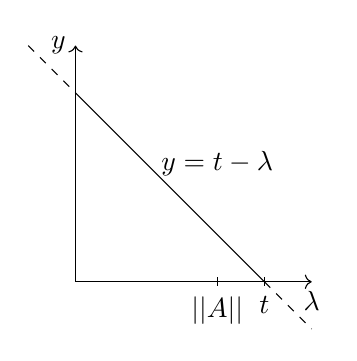
\begin{tikzpicture}[scale=0.6]
        \draw[->] (0,0) -- (5,0) node[left, below]{$\la$};
        \draw[->] (0,0) -- (0,5) node[left]{$y$};
        \draw (3,0.1) --(3,-0.1) node[below]{$||A||$};
        \draw (4,0.1) --(4,-0.1) node[below]{$t$};
        \draw (0,4) -- (4,0); %node[midway,below]{$y=t-\la$};
        \node at (3,2.5) (a) {$y=t-\la$};
        \draw[dashed] (-1,5) -- (0,4);
        \draw[dashed] (4,0) -- (5,-1);
    \end{tikzpicture}
    \caption{  } 
    %\label{}
\end{figure}    
From the continuous function calculus (in $\tAs$) we get
\[ ||tI-A|| = ||f(A)|| \underset{\text{isometric map}}{=} ||f||_{\infty} 
    = \sup\{|t-\la| : \la \in \Sp(A) \} \leq t  \]
$(ii) \implies (iv) \implies (iii)$ is obvious. 

$(iii)\implies (i)$. Assume $(iii)$ holds.
Then we know that 
\[\Sp(A) \subset \R \cap \{ \la \in \C : |\la|\leq ||A|| \}
\subseteq [-||A|| ,||A||] \subseteq [-t,t]
\]
As above we get that 
$||tI - A || = \sup\{|t-\la|: \la \in \Sp(A)\}$.
Using the assumption, we get that 
$\sup\{|t-\la| : \la \in \Sp(A)\} \leq t$ and we see that all $\la \in \Sp(A)$
have to be non-negative. 
\end{proof}

\begin{proposition}
\begin{enumerate}[(1)]
    \leavevmode
    \item Let $A,B \in \As^+$, $\la \geq 0$. Then $A+B \in \As^+$ and 
    $\la A \in \As^+$.

    \item $\As^+ \cap (-\As^+) = \{0\}$. 

    \item $\As^+$ is (norm) closed in $\As$ and therefore in $\Assa$.

\end{enumerate}   
\begin{proof}
    $(1)$ Using the lemma, we get that 
    $||\,||A|| I -A|| \leq ||A||$, $||\, ||B|| I - B || \leq ||B||$ (using the 
triangle inequality). 
    \[ ||\,\ub{(||A|| +||B||)}_{t} I - (A+B) || \leq ||A|| + ||B|| = t \]
    since $||A+B|| \leq ||A|| + ||B|| = t$. We can use the lemma again to conclude that
    $A+B \geq 0$. The proof that $\la A \in \As^+$ is elementary.

    $(2)$ Assume that $A \in \As^+\cap (-\As^+)$. Then we have $\Sp(A)\subseteq[0,\infty)$ 
and $\Sp(A)\subseteq (-\infty,0]$, so $\Sp(A) = \{0\}$. But $A$ is self adjoint, 
so we get $||A|| = r(A) = 0$ i.e. $A = 0$.

$(3)$ Assume $\{A_n\}_{n\in\N} \subseteq \As^+$, $A_n\to A \in \As$ in norm.
Then $A \leftarrow A_n = A_{n}^{*} \to A^{*}$, since the $*$-operation is norm 
continuous (in fact isometric), so $A = A^*$.
Moreover 
\begin{align*}
    ||\,||A||I-A||&\leq ||\,(||A|| -||A_n||)I|| + ||\,||A_n|| I - A_n|| + 
    ||A_n - A|| \\
    &\leq ||A|| - ||A_n|| + \ub{||A_n ||}_{\text{using lem.}} + ||A_n - A|| \\
    &\leq ||A_n - A|| + ||A_n|| + ||A_n-A|| \\
    &\leq 2||A_n-A|| + ||A_n|| \to ||A||
\end{align*}
i.e. $||\,||A|| I - A || \leq ||A||$. Hence $A\geq 0$ using again the lemma
\end{proof}
\end{proposition}
\begin{proposition}
    Assume $A \in \Assa$. Then there exits elements $A^+, A^- \in \As^+$ such that 
    $A = A^+ -A^-$ and $A^+A^- = 0$.
\end{proposition}
\begin{proof}
    We define $\Id^{\pm} \colon \Sp(A) \to [0,\infty)$, by 
    $\Id^{\pm}(\la) = \max\{\pm \la, 0\}$ for $\la \in \Sp(A)$.
    Note that $\Id^{\pm} (0) = 0$, so we can set $A^{\pm} =\Id^{\pm}(A) \in \As$.
    Then we can use that $\Id = \Id^{+} - \Id^{-}$ and $\Id^+ \Id^{-}=0$.
\end{proof}

\begin{definition}
    For $A,B \in \Assa$, we define $A \leq B$ to mean that $B-A \geq 0$. It follows 
    easily from the properties of $\As^+$ we have shown that $\leq$ is a
    partial order on $\Assa$.
\end{definition}
\begin{example}
    Assume $A \in \As^+$, $||A|| \leq 1$. Then $A^2 \leq A$. Indeed, we have that 
    $\Sp(A) \subseteq [0,1]$. So the function $f\colon \Sp(A)\to \R$ 
defined by $f(\la) = \la - \la^2$ is non-negative. Hence 
$\Sp(A-A^2) = \Sp(f(A)) = f(\Sp(A)) \subseteq [0,\tfrac{1}{4}]$, since $A-A^2 \in \Assa$
we get $A-A^2 \geq 0$.
\end{example}

\begin{lemma}
    For $R \in \As$ and $R^*R \in -\As^+$. Then $R =0$.
\end{lemma}
\begin{proof}
    The assumption says that $\Sp(-R^*R) \subseteq [ 0, \infty)$. Hence, using 
    exercise 9, we get that $\Sp(-RR^*)\cup\{0\} = \Sp(-R^*R)\cup \{0\}
    \subseteq [0,\infty)$. It follows that $-RR^* \geq 0$.
    Now write $R = S + iT$, $S,T \in \Assa$. Then 
    \begin{align*}
    R^*R+RR^* &= (S-iT)(S+iT) + (S+iT)(S-iT) \\
    &= S^2 -iTS + iST + T^2 + S^2 + iTS -iST + T^2\\
    &= 2S^2 + 2T^2
    \end{align*}    
    Now $S^2$ and $T^2$ are positive, so 
    \[R^* R = 2S^2 + 2T^2 + (-RR^*) \geq 0\]
    Hence $R^*R \in \As^+ \cap (-\As^+) = \{0\}$ (cf. previous proposition).
    So $||R||^2 = ||R^*R|| = 0$ i.e. $R=0$.

\end{proof}

\begin{theorem}
    Let $A \in \As$. Then $A \geq 0$ if and only if $A = B^*B$
for some $B \in \As$, so $\As^+ = \{ B^*B : B \in \As \}$.
\end{theorem}
\begin{proof}
    If $A\geq 0$, then $A = A^{1/2}A^{1/2} = B^*B$, with $B = A^{1/2}$, with 
$A^{1/2}$ is self adjoint. 

Conversely, assume $A = B^*B$, $B \in \As$. Then $A \in \Assa$, moreover we have 
seen in previous proposition that $A = A^+ -A^-$ where $A^{\pm}  = \Id^{\pm}(A)$,
so $A^+A^- = 0$, $A^+,A^- \in \As$.

Define $R = BA^-$. Then we have
\begin{align*}
    R^*R &= A^-B^*BA^- = A^-(A^+-A^-)A^- \\
         &= A^- \ub{A^+A^-}_{0} - (A^-)^3 = - (A^-)^3
\end{align*}
since $\Sp((A^-)^3) = \Sp(A^-)^3 \subseteq [0,\infty)$, we have
$(A^-)^3 \geq 0$. Hence $R^*R \in -\As^+$.
The lemma gives that $R=0$, which in turn gives that $(A^-)^3 = 0$ 
(here we use that $A^-$ is self-adjoint and not nilpotent).  
Thus we get $||A^-|| = r(A^-) = 0$ i.e. $A^{-} = 0$, so $A = A^{+} \in \As^+$
as desired. 
\end{proof}

\begin{proposition}
    A unital $C^*$-algebra, $A,B \in \As^+ \cap GL(\As)$. Then 
$A \leq B \implies B^{-1} \leq A^{-1}$.
\end{proposition}
\begin{proof}
    Assume $A \leq B$. The other assumption says that 
    $\Sp(A) \subseteq (0,\infty)$ and $\Sp(B) \subseteq (0,\infty)$. 
    We can form $A^{-1/2}$ and $B^{-1/2}$ in $\As$, by applying the 
    function $t \mapsto t^{-1/2}$ defined on $\Sp(A)$ (resp. $\Sp(B)$).
    Note that $A^{-1/2}, B^{-1/2} \in \As^+$.
    Using ex 11, we get that $B^{-1/2}AB^{-1/2} \leq B^{-1/2}BB^{-1/2} = I$. 
    Hence $(A^{1/2}B^{-1/2})^* A^{1/2}B^{-1/2} \leq I$. 
    From ex 7b we get that $||A^{1/2}B^{-1/2} || \leq 1$. This gives that
    $||(A^{1/2}B^{-1/2})^* || \leq 1$, hence $||B^{-1/2}B^{1/2}|| \leq 1$. 
    By ex 7b we now get 
    \begin{align*}
        (B^{-1/2}A^{1/2})^* B^{-1/2}A^{1/2} &\leq I \\
        A^{1/2}B^{-1/2} B^{-1/2}A^{1/2} &\leq I \\
        A^{1/2}B^{-1} A^{1/2} &\leq I 
    \end{align*}
Using ex. 11 we get 
\begin{align*}
    A^{-1/2} (A^{1/2}B^{-1}A^{-1/2})A^{-1/2} &\leq A^{-1/2}IA^{-1/2} = A^{-1} \\
    B^{-1} &\leq A^{-1}
\end{align*}
\end{proof}

\section{Approximate units in non-unital $C^*$-algebras}
\begin{definition}
    An (increasing) approximate unit (or identity) in a non-unital 
$C^*$-algebra $\As$ is a net $\{e_{\al}\}$ of self-adjoint elements in $\As$
satisfying 
\begin{enumerate}[(i)]
    \item $e_{\al} \geq 0$, $||e_{\al}|| \leq 1$ for all $\al$.
    \item $\al \preceq \beta$ implies $e_{\al} \leq e_{\beta}$.
    \item $\lim_{\al} ||Ae_{\al} - A|| = \lim_{\al}||e_{\al}A - A|| = 0$
    for all $A \in \As$.
\end{enumerate}

\begin{theorem}
    Any non-unital $C^*$-algebra has an approximate unit. 
\end{theorem}
\begin{proof}
    Let $\Is = \{\text{all finite non-empty subset of $\Assa$}\}$ ordered by 
set inclusion. For each $n \in \N$, define $f_n \colon [0,\infty) \to [0,1)$
by 
\[f_n(t) = \frac{nt}{1+nt} \]
Since $f_n$'s are continuous on $[0,\infty)$ and $f_n(0)= 0$ 
for all $n \in \N$, we can apply (the restriction of $f_n$ on any 
element $A\in \As^+$, by considering $f_n\lvert_{\Sp(A)}$) and 
obtain an element in $\As^+$. We will denote this element by $f_n(A)$.
For any $\al = \{A_1, \ldots , A_n\} \in \Is$  we define
$e_{\al} = f_n(A_{1}^{2}+ \ldots + A_{n}^{2})$. We now check that $(i)$, $(ii)$ and 
 $(iii)$ holds. 
\begin{enumerate}[(i)]
    \item Let $\al$ be as above. Since $A_{1}^{2} + \cdots + A_{n}^{2} \geq 0$
we get that $f_n(A_{1}^{2}+ \cdots + A_{n}^{2}) \geq 0$. 
Moreover $\Sp(e_{\al}) = f_n (\Sp(A_{1}^{2}+ \cdots + A_{n}^{2})) \subseteq [0,1)$,
so $||e_{\al}|| \leq 1$.

\item 
Consider $\al \leq \beta$ in $\Is$. So let $\al$ be as above and assume 
$\beta = \{A_1, \ldots, A_m\}$ where $n \leq m$. To show that 
$e_{\al} \leq e_{\beta}$ it suffices to show that 
$I-e_{\beta} \leq I -e_{\al}$ (in $\tAs$). Since 
$1 - f_k(t) = \frac{1}{1+kt}$ for all $t \geq 0$ and all $k \in \N$
it is the enough to show that 
\[
\(I + m(A_{1}^{2}+ \cdots + A_{m}^{2}) \)^{-1} \leq 
\(  I + n (A_{1}^{2}+ \cdots + A_{n}^{2}) \)^{-1}
\]
But using the previous proposition this inequality will follow if we can 
show that 
\[
I + n(A_{1}^{2}+ \cdots + A_{n}^{2}) \leq I + m(A_{1}^{2}+ \cdots + A_{m}^{2})
\]
This inequality follows immediately using that $\As^+$ is a cone.  

\item 
Assume $A^* = A \in \As$ and $n \in \N$.
Consider $\al = \{A_1, \ldots, A_n\}$ where we choose $A_1 = A$.
Let  $\beta = \{A_1, \ldots, A_m\}$, $m \geq n$. Then 
$A^2 \leq A_{1}^{2} + \cdots + A_{n}^{2}$, so 
exercise 11 gives 
$(I - e_{\beta} )(A^2) (I -e_{\beta})\leq (I -e_{\beta})(A_{1}^{2} + \cdots +
A_{n}^{2})(I -e_{\beta})$. Set now 
$g_m(t) = (1-f_m(t))t (1-f_m(t)) = \frac{t}{(1+mt)^2}$.
We have 
\[ (I - e_{\beta} )(A^2) (I -e_{\beta})\leq 
g_m(A_{1}^{2} + \cdots + A_{n}^{2})
\]
since $g_m(t) \leq \frac{1}{4m}$ for all $t \geq 0$ we get that
\begin{align*}
    (I - e_{\beta} )(A^2) (I -e_{\beta}) &\leq \frac{1}{4m} I \\
    (A-e_{\beta}A)^* (A - e_{\beta}A) &\leq \frac{1}{4m} I
\end{align*}
Using exercise $7b$ we deduce that 
$||2\sqrt{m} (A -e_{\beta}A)|| \leq 1$, so $||A-e_{\beta}A|| \leq
\frac{1}{2\sqrt{m}} \leq \frac{1}{2\sqrt{n}}$.
So given $\eps > 0$, we can choose $n$ such that $\tfrac{1}{2\sqrt{n}} \leq \epsilon$
we then get $||A-e_{\beta}A||< \eps$ for all $\beta \succeq \al$ for $\al$ as 
chosen before. So $||A-e_{\beta}A || \to 0$. Hence 
$||A-Ae_{\beta}|| = ||(A - Ae_{\beta})^*|| = ||A-e_{\beta}A|| \to 0$.
This shows $(iii)$ $A \in \Assa$. If $A \not\in \Assa$, we can write 
$A = S + iT$ where $S,T \in \Assa$ and apply what we have done to $S$ and $T$.

\end{enumerate}

\end{proof}


\begin{note}
\leavevmode
\begin{enumerate}[(1)]
    \item If $\As$ is unital, then $e_{n}  =I$ for all $n \in \N$, satisfies 
all conditions for an approximate unit in $\As$.

\item For $\As = C_{0}(\R)$ or $\As = \Ks(H)$ one can describe 
explicitly some natural approximate units (cf. Exercise for next week)

\item If $\As$ is a separable, then one can pick an approximate unit in 
$\As$ with countable index set. 
($C^*$-algebras with this property is called $\sigma$-unital. For proof, see 
Murphy)

\end{enumerate}    

\end{note}

\end{definition}


\section{Ideals and quotients}
\begin{proposition}
    Let $\Js$ be a norm closed ideal in a $C^*$-algebra $\As$. Then $\Js$ is self-adjoint ($B \in \Js \implies B^* \in \Js$). 
Hence $\Js$ is a $C^*$-subalgebra. 
\end{proposition}
\begin{proof}
    Let $\Js^* = \{B^* : B \in \Js\}$ and $\Ks = \Js\cap \Js^*$. Note that 
    $\Ks$ is nonempty since $B^*B \in \Ks$, for all $B\in \Js$ (using that $\Js$ is an ideal),
so $B^*B \in \Js$, but $B^*B$ is self adjoint so $B^*B \in \Js^*$.
Moreover one easily verifies that $\Ks$ is a $C^*$-subalgebra of $\As$.
So we may pick an approximative unit $\{e_{\al}\}$ for $\Ks$. Since 
$\Ks \subseteq \Js$, we have $e_{\al} \in \Js$ for all $\al$. Let 
$B \in \Js$. We then have 
\begin{align*}
    ||B-e_{\al}B||^2 &=
    ||B(I-e_{\al})||^2 = ||(I-e_{\al}) B^*B (I - e_{\al})|| \\
    &\leq \ub{||I-e_{\al}||}_{\leq 1} ||\ub{B^*B}_{\in \Ks}(I-e_{\al})|| \to 0
\end{align*}
where $I$ is the unit in the unitization if $\As$ is non-unital and we use that 
$\Sp(I-e_{\al})\subseteq [0,1]$. So $Be_{\al} \to B$.
Hence
\begin{align*}
||B^* - \ub{e_{\al}}_{\in \Js}B^* || = ||(B-Be_{\al})^* ||   = ||B-Be_{\al}|| \to 0 
\end{align*}
so $B^* \in \Js$ (since $\Js$ is closed).
\end{proof}


Consider a closed ideal $\Js$ in a $C^*$-algebra $\As$. We know that $\As/\Js$
is a Banach algebra w.r.t the quotient norm.
\begin{align*}
    ||A+\Js|| &= \inf\{ ||A-B|| : B\in \Js \} \\
              &= \inf\{ ||A+B|| : B\in \Js \}
\end{align*}
Since $J$ is self-adjoint, we may define a $*$-operation on $\As/\Js$ by
\[ (A + \Js)^* = A^* + \Js \quad \text{for all } A \in \As.\]
This is well defined since 
$A +\Js = A' + \Js$ i.e. $A-A' \in \Js$, then 
$A^* - (A')^* \in \Js^* = \Js$, so $A^* + \Js = (A')^* + \Js$.
Moreover it is trivial to check that this is a involution on 
$\As/\Js$, so $\As/\Js$ is a $*$-algebra.

\begin{theorem}
    $\As /\Js$ is a $C^*$-algebra.
\end{theorem}
\begin{proof}
    It only remains to show that the $C^*$-equality holds. As we have seen at
another occasion, it suffices to show that 
\begin{align*}
    ||A+\Js||^2 \leq ||(A + \Js)^*(A+ \Js)||\quad \text{ for all } A \in \As.
\end{align*}
Let $\{e_{\al}\}$ be an approximative unit to $\Js$. Observe that for 
$A \in \As$ then $||A + \Js|| = \lim_{\alpha}||A-Ae_{\al}||$. 

Indeed, let $\eps > 0$ and choose $B \in \Js$ such that 
$||A+B|| \leq ||A+\Js|| + \tfrac{\eps}{2}$. Next choose $\al_0$ such that 
$||B-Be_{\al}|| \leq \tfrac{\eps}{2}$ for all $\al \succeq \al_0$. 
Then for any $\al \succeq \al_0$, we get
\begin{align*}
    ||A+\Js|| &\leq ||A-Ae_{\al}|| \leq ||(A+B)(I-e_{\al})|| + ||B(I-e_{\al})|| \\
&\leq ||A+B|| + \tfrac{\eps}{2} \leq ||A+\Js|| + \tfrac{\eps}{2}+ \tfrac{\eps}{2}.
\end{align*}
It follows that the formula holds. Using it we get that for any $A \in \As$,
we have
\begin{align*}
    ||A+\Js||^2 &= \lim_{\al} ||A-Ae_{\al}||^2 = \lim_{\al} ||(I-e_{\al})A^*A (I-e_{\al})||\\
\end{align*}
As
\begin{align*}
    ||(I-e_{\al})A^*A (I-e_{\al})|| \leq ||A^*A (I-e_{\al})|| = ||A^*A-A^*Ae_{\al}|| \to || A^*A + \Js|| 
\end{align*}
Hence 
\begin{align*}
||A + \Js||^2 \leq ||A^*A + \Js|| = ||(A + \Js)^*(A+\Js)||
\end{align*}
as desired. 
\end{proof}


\begin{corollary}
    Let $\varphi \colon \As \to \Bs$ be a $*$-homomorphism between two 
$C^*$-algebras. Then $\varphi(\As)$ is a $C^*$-subalgebra of $\Bs$, which 
is $*$-isomorphic to $\As /\ker \varphi$. 
\end{corollary}
\begin{proof}
    We have seen that $\varphi$ is a bounded i.e. continuous so $\ker\varphi$
is a closed ideal of $\As$ and we may form $\As/\ker\varphi$.
Now the map $\bar{\varphi}\colon \As/\ker\varphi \to \Bs$ given by
$\bar{\varphi}(A + \ker\varphi) = \varphi(A)$ for $A \in \As$ is 
well defined because $A-A' \in \ker\varphi$ implies 
$\varphi(A) = \varphi(A')$.
Moreover $\bar{\varphi}$ is injective (by construction) and 
it is elementary to see that $\bar{\varphi}$ is a $*$-homomorphism. 
Then we know that $\bar{\varphi}$ is isometric. This give that 
$\varphi(\As) = \bar{\varphi} (\As/\ker\varphi)$ is complete, 
and therefore closed. Since $\varphi(\As)$ is a $*$-subalgebra of $\Bs$ we
get that it is a $C^*$-subalgebra of $\Bs$. 
Finally $\bar{\varphi}\colon \As/\ker\varphi \to \varphi (A)$
is a $*$-isomorphism.
\end{proof}

\begin{example}
Let $\As, \Bs$ be two $C^*$-algebras. We can then form their
\emph{direct sum} $\As \oplus \Bs = \As \times \Bs$ (as sets) and 
define operations by 
\begin{align*}
    (A,B)+(A',B') &= (A+A',B+B') \\
    (A,B)^* &= (A^*, B^*) \\
    \la (A,B) &= (\la A, \la B) \\
    (A,B)(A',B') &= (AA', BB') \\
    ||(A,B)|| &= \max\{||A||, ||B||\}.
\end{align*}    
Then $A\oplus B$ is a $C^*$-algebra (check!).
Define
\begin{align*}
    \pi_1 \colon \As\oplus \Bs \to \As && \pi_{1} (A,B) = A \\
    \pi_2 \colon \As\oplus \Bs \to \Bs && \pi_{2} (A,B) = B \\
\end{align*}
Then $\pi_i$ are $*$-homomorphisms with 
\begin{align*}
    \ker \pi_1 = \{0\} \oplus \Bs \simeq \Bs \quad\text{ and } \quad   
    \ker \pi_2 = \{0\} \oplus \As \simeq \As    
\end{align*}
so $\As \oplus\Bs /\ker \pi_1 \simeq \As$ and $\As \oplus\Bs /\ker \pi_2 \simeq
\Bs$.

\end{example}

\begin{proposition}
    Assume $\Js$ is a closed ideal in a $C^*$-algebra $\As$ and 
$\Is$ is a closed ideal in $\Js$. Then $\Is$ is a closed ideal in $\As$.
\end{proposition}
\begin{proof}
    Since $\Is^+$ spans $\Is$ it suffices to show that given $A\in \As$ and 
$B \in \Is^+$ we have $AB, BA \in \Is$. Let 
$\{e_{\al}\}$ be an approximate unit for $\Js$. Then we have 
$B^{1/2} \in \Is \subseteq \Js$, so $e_{\al}B^{1/2} \to B^{1/2}$.
Then we can write $AB = AB^{1/2}B^{1/2} = 
\lim_{\al} \ub{Ae_{\al}B^{1/2}}_{
\Js} \ub{B^{1/2}}_{\in \Is} \in \Is $ since $\Is$ is a closed ideal in $\Js$.
This implies that we also have $A^*B \in \Is$. Hence $BA = (A^*B)^* \in \Is^* = \Is$.


\end{proof}

\begin{corollary}
    Let $H$ be a Hilbert space. Then $\Ks(H)$ is a \emph{simple} $C^*$-algebra, meaning 
that $\Ks(H)$ and $\{0\}$ are the only closed ideals in $\Ks(H)$.
\end{corollary}
\begin{proof}
    Let $\Is$ be a non-zero ideal in $\Ks(H)$ (is a closed ideal in $\Bs(H)$). 
    So $\Is$ is a closed ideal in $\Bs(H)$. But then we know that 
    $\Fs(H) \subseteq \Is$. Hence $\Ks(H)  = \ol{\Fs(H)}^{||\cdot||} \subseteq
    \Is \subseteq \Ks(H)$ i.e. $\Ks(H) = \Is$.
\end{proof}

\section{On positive linear functionals and states on $C^*$-algebras}
We let $\As$ denote a $C^*$-algebra.
\begin{definition}
    A linear functional $\varphi\colon \As \to \C$ is called \emph{positive}
when $\varphi(A)\geq 0$ for all $A \in \As^+$. In which case we write 
$\varphi \geq 0$. In other words $\varphi(B^*B) \geq 0$ for all $B \in \As$.
\end{definition}
Note that if $\varphi,\psi$ are positive linear functionals on  $\As$ and 
$\la \geq 0$, then $\varphi + \psi \geq 0$ and $\la\varphi \geq 0$ (cone).

Note also that $\varphi \geq 0$ if and only if $\varphi(A)\leq \varphi(B)$
for all $A,B \in \Assa$ such that $A \leq B$. 
\begin{example}
    $\Om$ compact Hausdorff space, $\mu$ finite Borel measure on $\Om$.
Set $\As = C(\Om)$. Then 
\[ \varphi_{\mu}(f) \coloneqq \int_{\Om} f \d \mu , \quad f \in \As\]
gives a positive linear functional on $\As$, (and the
Riesz representation theorem says that $\mu \mapsto \varphi_{\mu}$ is a 
bijective correspondence).

Note that 
\[ |\varphi_{\mu}(f)| \leq \int_{\Om}|f|\d \mu \leq ||f|| \mu(\Om) \]
for all $f \in \As$, and $\varphi_{\mu} (1_{\Om}) = \mu(\Om)$,
so $\varphi_{\mu}$ is bounded with $||\varphi_{\mu}|| = \mu(\Om)$.
\end{example}
\begin{example}
    $H$ Hilbert space, $\As = \Bs(H)$, $\xi \in H$.
Let $\om_{\xi}\colon \As \to \C$ be defined by 
$\om_{\xi}(A) = \ind{A\xi,\xi}$, $A \in \As$. Then 
$\om_{\xi}(B^*B)= \ind{B^*B\xi,\xi} = \ind{B\xi,B\xi} = ||B\xi||^2 \geq 0$
for all $B \in \As$, so $\om_{\xi}$ is a positive linear functional on $\As$.

Note that $|\om_{\xi}(A)| \leq ||A\xi||\,||\xi|| \leq ||A||\,||\xi||^2$ 
and $\om_{\xi}(I_{H}) = ||\xi||^2$, so $\om_{\xi}$ is bounded with $||\om_{\xi}|| = ||\xi||^2$.

\end{example}

\begin{example}
    Assume $\varphi$ is multiplicative (not non-zero as for characters) linear 
functional from $\As$ to $\C$. Then we have seen that $\varphi$ is self 
adjoint, meaning that $\varphi(A^*) = \ol{\varphi(A)}$ (proof Gelfand-Neumark)
in the case when $\As$ is unital, but by extending $\varphi$ to $\tAs$ when $\As$
is non-unital, the argument goes through, so we get 
\[\varphi(B^*B) = \varphi(B^*)\varphi(B) = |\varphi(B)|^2 \geq 0, \quad
\text{for all }B\in \As.\]
so $\varphi \geq 0$. Note that $\varphi$ is bounded with $||\varphi|| = 1$
if $\varphi \neq 0$.
[We have seen this when $\As$ is unital check this when $\As$ is non-unital.]
\end{example}

An important observation that will be used later is the following: 
Let $\varphi$ be a positive linear functional on $\As$. Then we can define a 
map $\ind{\cdot, \cdot}_{\varphi}\colon \As\times \As \to \C$ by
$\ind{A,B}_{\varphi} = \varphi(B^*A)$ for $A, B \in \As$.  
Then it is easy to check that $\ind{\cdot,\cdot}_{\varphi}$ gives
a semi-inner product on $\As$ (like a inner product, except that we do not 
require  $\ind{B,B}_{\varphi} = 0 \implies B = 0$).

But the \emph{Cauchy-Swartz inequality} still holds i.e. we have
$|\ind{A,B}_{\varphi}|^2\leq \ind{A,A}_{\varphi}\ind{B,B}_{\varphi}$ for all $A,B \in \As$.
Which says that 
$|\varphi(B^*A)|^2 \leq \varphi(A^*A)\varphi(B^*B)$ for all $A,B\in \As$.

\begin{proposition}
    Let $\varphi$ be a positive linear functional on $\As$. Then $\varphi$
is bounded. If $\As$ is unital, then $||\varphi|| = \varphi(I)$ where $I$
is the unit of $\As$. If $\As$ is non-unital and $\{e_{\al}\}$ is an approximative 
unit for $\As$, then $||\varphi|| = \lim_{\al} \varphi(e_{\al})$.
\end{proposition}
\begin{proof}
\begin{enumerate}[(1)]
    \item 
    Assume $\As$ is unital (Most for fun). Let $A \in \As^+$. Then $A \leq ||A||I$
so $\varphi(A)\leq \varphi(||A|| I) = ||A|| \varphi(I)$. Let $A \in \As$. 
Then 
\[|\varphi(A)|^2 = |\varphi(I^*A)|^2 \underset{\text{C.S}}{\leq} 
\varphi(A^*A)\varphi(I^*I) \leq ||A^*A||\varphi(I)^2\]
which gives that $|\varphi(A)|\leq \varphi(I)||A||$ for all $A \in \As$. 
It follows that $\varphi$ is bounded with $||\varphi|| = \varphi(I)$.

\item Assume $\As$ is non-unital. Let $(\As^+)_1 = \As_{1}^{+} = \{A \in \As^+: ||A||\leq 1\}$.
Then we claim that 
\[ M = \sup\{ \varphi(A) : A \in \As^{+}_{1} \}< \infty. \]
Assume $M$ was not finite. Then we can pick a sequence $\{A_n\} \subseteq \As_{1}^{+}$
such that $\varphi(A_n) \geq n$ for all $n \in \N$. Consider the series 
\[ \sum_{n=1}^{\infty}\frac{1}{n^2} A_n \]
which is absolutely convergent (Banach space), hence convergent in $\As$ to some $A \in \As$.
Now 
\[B_m = \sum_{n=1}^{m}\frac{1}{n^2}A_n \geq 0 \quad \text{for all }m \in \N\]
so $A \in \As^+$, since $\As^+$ is closed. 

moreover $A \geq B_m$ for all $m \in \N$, so we get 
\[\varphi(A)\geq \varphi(B_m) = \sum_{n=1}^{m} \frac{1}{n^2}\vphi(A_n) \geq \sum_{n=1}^{m} 
\frac{1}{n^2}n  = \ub{\sum_{n=1}^{m} \frac{1}{n}}_{\infty} \quad \text{for all }m\in \N  \]
which implies that $\varphi(A)=\infty$ which is impossible. 

Let $A \in \As_1$. Write $A = (B^+-B^-) + i (C^+-C^-)$ for $B^{\pm},C^{\pm}\in \As_{1}^{+}$.
We then get 
\[ |\varphi(A)| \leq \varphi(B^+) + \varphi(B^-) + \varphi(C^+) + \varphi(C^-)\leq 4M\]
This shows that $\varphi$ is bounded. 

Let $\{e_{\al}\}$ be an approximative unit for $\As$ and consider the net 
$\{\varphi(e_{\al})\}$. It is an increasing net of non-negative real numbers, which 
is bounded above by $||\varphi||$. (Since $\varphi$ is bounded) So $
\delta \coloneqq \lim_{\al} \varphi(e_{\al})$ exist and $\delta \leq ||\varphi||$.
For $A \in \As_1$, we have 
\[|\varphi(\ub{e_{\al}}_{=e_{\al}^{*}}A)|^2\leq \varphi(\ub{A^*A}_{\in
\As_{1}^{+}})\varphi(\ub{e_{\al}^*e_{\al}}_{e_{\al}^{2}}) \leq
\varphi(e_{\al})||\varphi||\leq \delta ||\varphi||\]
where we used that $0 \leq e_{\al}$, $||e_{\al}|| \leq 1$ i.e. $e_{\al}^{2}\leq e_{\al}$.
We get 
\[ |\varphi(A)|^2 = \lim_{\al}|\varphi(e_{\al}A)|^2 \leq \delta||\varphi|| \]
Taking the supremum over all $A \in \As_1$, this implies that $||\varphi||^2 \leq \delta ||\varphi||$ which  implies that
$||\varphi||\leq \delta$. All together $\delta = ||\varphi||$ as desired. 
\end{enumerate}
\end{proof}


\begin{proposition}\leavevmode
\begin{enumerate}[(1)]
    \item 
    Let $\varphi \in \As^*$. If $\As$ is unital and $||\varphi|| = \varphi(I)$, 
then $\varphi \geq 0$.
\item More generally, assume $||\varphi|| = \lim_{\al}\varphi(e_{\al})$ for some
approximative unit $\{e_{\al}\}$ for $\As$. Then $\varphi \geq 0$.

\end{enumerate}

\end{proposition}
\begin{proof}
\begin{enumerate}[(1)]
    \item 
    Assume $\As$ is unital and $||\varphi|| = \varphi(I)$. We can assume that
$||\varphi||= 1$. (otherwise, we just look at $\psi =
\frac{1}{||\varphi||}\varphi$, when $\varphi\neq 0$). Assume for contradiction
that $\varphi$ is not positive, so there exists some $A\in \As^+$ such that
$\varphi(A)\not\in [0,\infty)$. 
Since $\Sp(A) \subseteq [0,\infty)$ we can choose some $\la \in \C$
and $r> 0$ such that 
\begin{align*}
\varphi(A) &\not\in D(\la, r)\coloneqq \{ x \in \C: |\la -x|\leq r \} \\ 
\Sp(A) &\subseteq D(\la,r)
\end{align*}
Then we have $\Sp(A -\la I) \subseteq D(0,r)$ so $||A-\la I||\leq r$ and 
we also have 
\[ |\varphi(A-\la I)|  = |\varphi(A) - \la \varphi(I)| = 
|\varphi(A) - \la| > r\]
But we also have
\[ |\varphi(A-\la I)| \leq \ub{||\varphi||}_{=1} ||A-\la I ||\leq r \]
which is a contradiction. So $\varphi \geq 0$.

\item 
Assume $||\varphi|| = \lim_{\al}\varphi(e_{\al})$ for some approximate 
unit $\{e_{\al}\}$ for $\As$. We can assume $||\varphi||=1$.
As usual let 
\[ \tAs = \begin{cases} \As &\text{if $\As$ is unital}\\ &\text{The unitization of $\As$ otherwise } \end{cases}\]
and $I$ denotes the unit of $\tAs$.

By the Hahn-Banach theorem, we can extend $\varphi$ to $\tilde{\varphi} \in 
(\tAs)^*$ with $||\tilde{\varphi}|| = ||\varphi|| = 1$. 
Let $z = \tvphi(I)$. Then $|z| \leq ||\tvphi||\, ||I||  = 1$. Moreover 
$||2e_{\al} - I||\leq 1$ since $\Sp(e_{\al}) \subseteq [0,1]$ for all $\al$
so 
\[ |\tvphi(2e_{\al} - I)| \leq ||\tvphi|| \, ||2e_{\al} - I||\leq 1 \]  
Next we have $|\tvphi(2e_{\al} - I)| = |2\vphi(e_{\al}) - z| \to |2-z|$. 
Hence  $|2-z|\leq 1$.
So we get that $z = 1$, i.e. $\tvphi(I) = 1$.
So we have $||\tvphi|| = 1 = \tvphi(I)$. By the first part we get that 
$\tvphi \geq 0$, which implies that the restriction $\tvphi\lvert_{\As} = \vphi \geq 0$
\end{enumerate}
\end{proof}

Note:
The argument given in the proof of 2) shows that if $\varphi \geq 0$ on $\As$ 
(non-unital) then $\varphi$ has a unique extension $\tvphi$ to $\tAs$ such that 
$\tvphi\geq 0$ and $||\tvphi|| = ||\vphi||$, and $\tvphi$ is given by
$\tvphi(A + \la I) = \vphi(A) + \la ||\vphi||$. 

More generally we have:  

\begin{theorem}[Hahn-Banach for positive linear functionals]
   Assume $\As$ is a $C^*$-subalgebra of a $C^*$-algebra $\Bs$ and that 
$\vphi$ is a positive linear functional on $\As$. Then $\varphi$ may be 
extended to a positive linear functional $\vphi'$ on $\Bs$ such that 
$||\vphi|| = ||\vphi'||$.
\end{theorem}

\begin{proof}
    Again we may assume that $||\vphi||=1$. Set 
\[ \widetilde{\Bs} = \begin{cases} \Bs &\text{if $\Bs$ is unital}\\ &\text{The unitization of $\Bs$ otherwise } \end{cases}\]
and let $I$ denote the unit in $\tBs$.
Since $\vphi$ is bounded on $\As$ it can be extended using the Hahn-Banach theorem 
to a bounded linear functional $\tvphi$ on $\tBs$ such that $||\tvphi|| =
||\vphi|| = 1$. Set $z = \tvphi(I)$ so $|z| \leq 1$. Let $\{e_{\al}\}$ be an 
approximate unit for $\As$. Since $\vphi \geq 0$, we know that $\lim_{\al} \vphi(e_{\al}) = ||\vphi|| = 1$. As in the previous proof, we set 
\[\tvphi(2e_{\al} - I) \leq 1\]
where $\tvphi(2e_{\al} - I) \to |2-z|\leq 1 $. Hence 
$z = \tvphi(I) = 1$. So we have $||\tvphi|| = 1 = \tvphi(I)$. Part (1) of the previous proposition
gives $\tvphi\geq 0$.
Set $\vphi' = \tvphi\lvert_{\Bs}$. Then $\vphi'\geq 0$ and 
$\vphi'\vert_{\As} = \tvphi\lvert_{\As}  = \vphi$. Moreover 
$1 \leq ||\vphi|| \leq ||\vphi'|| \leq ||\tvphi|| =1$.
\end{proof}

\begin{proposition}
    Let $\phi, \psi$ be positive linear functionals on $\As$. Then 
    \[ ||\vphi +\psi || = ||\vphi|| + ||\psi|| \]
\end{proposition}
\begin{proof}
    Let $\{e_{\al}\}$ be an approximative unit for $\As$. Then 
    \begin{align*}
        ||\vphi +\psi|| = \lim_{\al} (\vphi+\psi)e_{\al} = \lim_{\al}\vphi e_{\al}
        + \lim_{\al} \psi e_{\al} = ||\vphi ||+||\psi||
    \end{align*}    
\end{proof}

\begin{definition}
    We set \[\Ks(\As) = \{ \vphi \in \As^* : \vphi\geq 0, ||\vphi||\leq 1 \}\]
    and 
    \[ \Ss(\As) = \{ \vphi \in \Ks(\As) : ||\vphi||=1 \} \]
    Elements of $\Ss(\As)$ are called \emph{states} and $\Ss(\As)$ are called the 
    \emph{state} space of $\As$. 
\end{definition}

As we will see soon $\Ss(\As) \neq 0$ when $\As \neq \{0\}$.
Note:  $\Ks(\As)$ and $\Ss(\As)$ are convex. This follows readily from the previous 
proposition. We will come back to $\Ks(\As)$ and $\Ss(\As)$ later. 
\begin{theorem}
    Assume $\As \neq \{0\}$ and let $A \in \As\setminus\{0\}$ be \emph{normal}.
    Then there exists $\vphi\in \Ss(\As)$ such that 
    $|\vphi(A)| = ||A||$. 
    Note that this implies that $||A|| = \sup\{ \vphi(A) : \vphi \in \Ss(\As)\}$.
    More generally we get 
    \[ ||B|| = \sup\{ |\vphi(B^*B)|^{1/2} : \vphi \in \Ss(\As)\}. \]

\end{theorem}

\begin{proof}
    Set 
\[\tAs = \begin{cases} \As &\text{if $\As$ is unital} \\&\text{the unitization if $\As$ is nonunital} \end{cases}\]
$I$ unit of $\tAs$. Since $||A||=r(A)$ and $\Sp(A)$ is compact, we get that 
there exists a $\la \in \Sp(A)$ such that $|\la| = ||A||$.
Let $\Cs$ denote the $C^*$-subalgebra of $\tAs$ generated by 
$A$ and $I$, which is commutative since $\As$ is normal. 
By Gelfand theory we get that there exits $\gamma \in \widehat{\Cs}$
such that $\gamma(A) = \la$ (recall that $\Sp_{\Cs}(A) = \Sp_{\tAs}(A) = \Sp_{\As}(A)$).
Let $\Bs$ be the $C^*$-subalgebra of $\Cs$ generated by $A$. Set $\psi=\gamma\lvert_{\Bs}$.
Then $\psi$ is a multiplicative linear functional and 
\[ |\psi(A)| = |\gamma(A)| = |\la| = ||A|| \neq 0, \] 
so $\psi\neq0$.
Hence $\psi\geq 0$, so $||\psi|| = \lim_{\al}\psi(e_{\al})$ for any approximative 
unit $\{e_{\al}\}$ for $\Bs$. But $\ub{\psi(A)}_{\neq 0} \lim_{\al}\psi(e_{\al}) 
= \lim_{\al}\psi(Ae_{\al}) = \psi(A)$, so $\lim_{\al}\psi(e_{\al})=1$.
Hence $||\psi||=1$. Now $\Bs$ is $C^*$-subalgebra of $\As$. By Hahn-Banach theorem 
for positive linear functional, we can extend $\psi$ to a positive linear functional 
$\vphi$ on $\As$ with $||\vphi|| = ||\psi|| = 1$.
So $\vphi \in \Ss(\As)$ and $|\vphi(A)| = |\psi(A)|=||A||$.
\end{proof}
Looking at the proof of this result, we see that we in fact prove that given 
$\la \in \Sp(A)$, then there exists $\psi \in \Ss(\As)$ such that $\psi(A) = \la$.

\begin{corollary}
    Let $\As \neq \{0\}$ be a $C^*$-algebra. Then we have 
\begin{enumerate}[(1)]
    \item $A =0$ if and only if $\vphi(A)=0$ for all $\vphi \in \Ss(\As)$.
    \item $A \in\Assa$ if and only if $\vphi(A)\in \R$ for all $\vphi \in \Ss(\As)$.
    \item $A \geq 0$ if and only if $\vphi(A)\geq 0$ for all $\vphi \in \Ss(\As)$.
\end{enumerate}
\end{corollary}
\begin{proof}

\begin{enumerate}[(1)]
    \item Assume $\vphi(A) =0$ for all $\vphi \in \Ss(\As)$, $A$ normal.
If $A\neq 0$ we can use the previous proposition to produce some $\vphi \in \Ss(\As)$
such that $|\vphi(A)| = ||A||$. Hence $A = 0$, a contradiction. 

If $A$ is not normal, write $A = B + iC$ where $C,B\in \Assa$. We then have 
$\ub{\vphi(B)}_{\in \R} + i\ub{\vphi(C)}_{\in \R} = 0$ for all $\vphi\in \Ss(\As)$,
so $B = C = 0$ by the first part i.e. $A = 0$.

\item We have seen that $(\implies)$ holds for any $\vphi\geq 0$ 
(by writing $A = A^+-A^-$ for $A^{\pm} \in \As^+$).

Conversly assume $\vphi(A) \in \R$ for all $\vphi \in \Ss(\As)$. 
Then we have $\vphi(A^*-A) = \ol{\vphi(A)}-\vphi(A) = \vphi(A)-\vphi(A) = 0$
for all $\vphi\in \Ss(\As)$. By $(1)$ we get $A^*-A=0$.

\item $(\implies)$ follows by def of positiveness for linear functionals.
For $(\impliedby)$  assume $\vphi(A)\geq 0$ for all $\vphi\in \Ss(\As)$. 
$(2)$ gives that $A \in \Assa$. Moreover, let $\la \in \Sp(A)$. By the proof of the previous
proposition we can find $\psi \in \Ss(\As)$ such that $\psi(A)= \la$.
Hence $\psi(A)\geq 0$ using the assumption, so $\Sp(A)\subseteq [0,\infty)$.
Hence $A\geq 0$.
\end{enumerate}

\end{proof}
\begin{definition}
    Let $\As$ be a $C^*$-algebra and let 
     $\vphi \in \As^*$. Then we define 
$\vphi^*\colon \As\to \C$ by $\vphi^*(A) = \ol{\vphi(A^*)}$, $A\in \As$.
\end{definition}

Then it is an easy exercise to check that 
$\vphi^* \in \As^*$ such that $||\vphi|| = ||\vphi^*||$
and $(\vphi^*)^* = \vphi$. Moreover for $\vphi,\psi \in \As^*$, $\la \in \C$ 
we have $(\vphi+\psi)^* = \vphi^* +\psi^*$ and $(\la\vphi)^* = \ol{\la}\vphi^*$.
Note that $\vphi \in \As^*$ is self-adjoint if and only if $\vphi = \vphi^*$.    
    
Moreover if $\psi \in \As^*$ we can write 
\[\psi = \ub{\frac{\psi + \psi^*}{2}}_{\text{self-adj.}} + i\ub{\(\frac{1}{2i} (\psi -\psi^*)\)}_{\text{self-adj.}}\] 
so any element of $\As^*$ is a linear combination of self-adjoint elements of
$\As^*$.  Note also that $\vphi \in \As^*$ is self-adjoint if and only if
$\vphi(\Assa) \subseteq\R$ (easy exercise). 

Hence if $\vphi$ is self-adjoint the its restriction $\vphi'$ to $\Assa$ takes
its value in $\R$. So $\vphi'$ is a linear functional on $\Assa$, considered 
as a real vector space.

Moreover $\vphi'$ is bounded with respect to the operator norm on $\Assa$ and
$||\vphi'|| = ||\vphi||$. 
\begin{proposition}
   Let $\vphi \in \As^*$ be  self-adjoint, so $\vphi(\Assa) \subseteq \R$. 
The restriction $\vphi'$ of $\vphi$ to $\Assa$ is then a linear functional on $\Assa$
(considered as a real vector space) and 
$\vphi'$ is bounded with $||\vphi'|| = ||\vphi||$. 
\end{proposition}
\begin{proof}
    We will first show that if $\vphi \in \As^*$, then  
\[ ||\vphi|| = \sup \{ |\Re\vphi(A)|:A\in \As, ||A|| \leq 1 \}  \]
Indeed, if $||A||\leq 1$, then 
$|\Re \vphi (A)| \leq |\vphi(A)| \leq ||\vphi|| ||A|| \leq ||\vphi||$ so 
$\sup \{ |\Re\vphi(A)|:A\in \As, ||A|| \leq 1 \} \leq ||\vphi|| $.
Let $A \in \As$, $||A||\leq 1$. Choose $\la \in \C$, $|\la|= 1$ such that 
$\la\vphi(A) \subseteq \R$. Then $\vphi(\la A) = \la \vphi(A) \in \R$, 
so $\vphi(\la A) = \Re \vphi(\la A)$.
Moreover 
\begin{align*}
    &|\vphi(A)| \underset{|\la|=1}{=} |\la \vphi(A)| = |\Re( \la\vphi(A) )|
    \underset{||\la A|| \leq ||A|| \leq 1}{\leq} \sup \{|\Re \vphi(B)| 
    : B\in \As,||B||\leq 1\} \\
%
    &\implies ||\vphi|| \leq \sup \{|\Re \vphi(B)| : B\in \As,||B||\leq 1\}
\end{align*}
We can now prove the lemma. 
If $A \in \Assa$, $||A||\leq 1$ then 
\begin{align*}
    |\vphi'(A)|\leq |\vphi(A)| \leq ||\vphi|| \quad \text{so } ||\vphi'||\leq||\vphi||.
\end{align*}
Consider now $A \in \As$, $||A||\leq 1$.
Write $A = B + iC$, $B = (A+A^*)/2$, $C = (A-A^*)/(2i)$, then 
$B,C \in \Assa$ and $||B||\leq ||A|| \leq 1$ and $||C||\leq||A||\leq 1$.
Moreover 
$\vphi(A) = \vphi(B) + i\vphi(C)$ since $\vphi$ is self-adjoint, so 
$\Re(\vphi(A)) = \vphi(B)  =\vphi'(B)$, so 
$|\Re \vphi(A)| = |\vphi'(B)| \leq ||\phi'||$
since $||B||\leq 1$, $B \in \Assa$.
Hence $\ub{\sup \{ |\Re \vphi(A)| : ||A||\leq 1, A\in \As\}}_{||\vphi||\text{
by our first obs.}} \leq ||\vphi'||$.

\end{proof}

We now set 
\[  (\As^*)_{\text{sa}} = \{ \vphi \in \As^* : \vphi^* = \vphi \}\]
If $X$ is a real normed space, we will denote its dual by $X^{\sharp}$.
What we have just seen is that we have a isometric linear map from 
$(\As^*)_{\text{sa}}$ into $(\Assa)^{\sharp}$ sending $\vphi$ to its restriction
$\vphi'$. It is easy to see that it is a bijection,
the inverse map can be defined as follows: 

If $\psi \in (\Assa)^{\sharp}$, then let $\tilde{\psi} \colon \As \to \C$ be 
given by 
\[ \tilde{\psi}(A) = \psi((A+A^*)/2) + i\psi((A-A^*)/(2i))  \]
Then one checks that $\tilde{\psi} \in (\As^*)_{\text{sa}}$ and
$\tilde{\psi}'=\psi$ on $\Assa$. Se we can identify 
$(\As^*)_{\text{sa}}$ with $(\Assa)^{\sharp}$ using this map. 

\section{The Jordan decomposition theorem}
Let $\vphi \in (\As^*)_{\sa}$. Then there exists 
positive linear functionals $\vphi^+$ and $\vphi^-$ on $\As$ such that 
$\vphi = \vphi^+ - \vphi^-$ and 
$||\vphi|| = ||\vphi^+|| + ||\vphi^-||$.
It can be show that $\vphi^+$ and $\vphi^-$ are uniquely determined by these
properties. 
\begin{proof}
\marginnote{$\Ks(\As)$ is weak$^*$ closed}
    Set $\Om = \Ks(\As) = \{\vphi \in \As^* : \vphi\geq 0, ||\vphi||\leq 1\}$.
    Note that $\Om$ is weak$^*$ closed subset of $(\As^*)_{1}$. Indeed, if 
    $\{\vphi_{\al}\}$ is a net in $\Om$ converging with respect to
    the weak$^*$ topology to some $\vphi \in (\As^*)_1$
    for any $A \in \As^+$ we have $\vphi(A) = \lim_{\al} \underset{\geq
    0}{\vphi_{\al}} (A)\geq 0$, since $\vphi_{\al}\geq 0$.
    So $\vphi\geq 0$ i.e. $\vphi \in \Om$, since $(\As^*)_1$ is weak$^*$ compact
    and Hausdorff we get that $\Om$ is weak$^*$ compact and Hausdorff. Now
    define a map $\theta \colon \Assa \to C(\Om,\R)$ by 
    \[ [\theta(A)](\vphi)\coloneqq \vphi(A) \quad \text{ for }A\in \Assa, \vphi\in \Om.\]
    $\theta$ is clearly well defined and linear. Moreover it is positive i.e.
    if $A\geq 0$, $[\theta(A)](\vphi) = \vphi(A)\geq 0$ for all $\vphi \in
    \Om$, so $\theta (A)$ is positive in $C(\Om,\R)$. It is also \ul{isometric:} 
    \marginnote{isometric, linear $\implies$ injective}
    For $A \in \Assa$ we have 
    \[ ||\theta(A)|| = \sup\{ \ub{|[\theta(A)](\vphi)|}_{\vphi(A)} : \vphi \in \Om \} 
    =\sup\{ \vphi(A) : \vphi \in \Om \} = ||A|| 
    \] 
    where we use the previous proposition. 
    Let us now consider $\vphi \in (\As^*)_{\sa}$ and its restriction 
    $\vphi'$ to $\Assa$ i.e. $\vphi' = \vphi\lvert_{\Assa}$.
    
    \begin{center}
        \begin{tikzcd}
            \As \arrow[d,no head] \arrow[r, "\vphi "] & \ar[d,no head] \mathbb{C} \\
            \Assa \ar[d, "\theta"] \ar[r,"\vphi'"] &\R \\
            \theta (\Assa) \subseteq C(\Om,\R) 
            \ar[ur, dashed,swap,"\psi =\vphi' \circ \theta^{-1}"]
            \ar[ur, bend right=120, swap, "\rho"]
    \end{tikzcd}
    \end{center}    


    Since $\theta(\Assa)$ is a subspace of $C(\Om,\R)$ and $\theta$ is injective,
    we can define $\psi \colon \theta(\Assa) \to \R$ by 
$\psi(\theta(A)) = \vphi'(A)$ for $A\in \Assa$ i.e. $\psi = \vphi' \circ \theta^{-1}$.
Then $\psi$ is linear and $|\psi(\theta(A))| = |\vphi'(A)| \leq
||\vphi'||\,\ub{||A||}_{=||\theta(A)||} $ for all $A \in \Assa$.
So $\psi$ is bounded with $||\psi|| \leq||\vphi'||$. On the other hand if $A
\in \Assa$, then
\[ |\vphi'(A)| = |\psi(\theta(A))| \leq ||\psi|| ||\theta(A)||\]
so $||\vphi'||\leq ||\psi||$. Hence 
$||\psi|| = ||\vphi'|| = ||\vphi||$. By the Hahn-Banach theorem we can extend
$\psi$ to $\rho \in C(\Om,\R)^{\sharp}$ with $||\rho || = ||\psi||$.
Now by the Riesz representation theorem, $\rho$ corresponds to a finite 
signed regular measure on $\Om$ which decomposes as $\nu =\nu^+-\nu^-$,
so we get that $\rho =\rho^+ - \rho^-$, where $\rho^{\pm}$ are positive linear functionals
on $C(\Om,\R)$. 

Now we can set $\vphi^{\prime\pm} = \rho^{\pm} \circ \theta \colon \Assa\to \C$, 
thus $\vphi^{\prime\pm} \in (\Assa)^*$, we denote the corresponding  
elements in $(\As^*)_{\sa}$ for $\vphi^{\pm}$.
Note that $\vphi^{\pm}\geq 0$, because 
for $A\geq 0$ we have $\vphi^{\pm}(A) = \vphi^{'\pm}(A) =
\rho^{\pm}(\ub{\theta(A)}_{\geq 0})\geq 0$. 
Note also that since $\rho = \rho^+ - \rho^-$ we also get $\vphi = \vphi^+ -\vphi^-$
and $\vphi' = \vphi^{'+} - \vphi^{'-}$. Finally we have 
 \begin{align*}
     ||\vphi|| &= ||\vphi'|| = ||\psi|| = ||\rho||\underset{\text{jord. dec. thm.}}{=}
    ||\rho^+|| + ||\rho^-|| \\ 
    &\geq ||\vphi^{'+}|| +  ||\vphi^{'-}||
 \geq ||\vphi^{+}|| +  ||\vphi^{-}||\geq ||\vphi||
\end{align*}
where we used that  $||\vphi|| = ||\vphi^+ + \vphi^-|| \leq ||\vphi^+|| + ||\vphi^-||$.
So $||\vphi|| = ||\vphi^-|| +||\vphi^+||$.
\end{proof}
\begin{corollary}
    Any $\varphi \in \As^*$ is a linear combination of positive linear functionals.
\end{corollary}

\section*{Representations of $C^*$-algebras}
\begin{definition}
    Let $H$ be a Hilbert space and let $\As$ be a $C^*$-algebra. 
    A $*$-homomorphism $\pi \colon \As \to \Bs(H)$ is called a \emph{representation} 
    of $\As$ on $H$ and we sometimes write $\pi \in \Rep(\As,H)$.
    $\pi$ is called \emph{faithful} when it is injective.
\end{definition}

\begin{example}\leavevmode
    \begin{enumerate}[(1)]
        \item If $\As$ is a $C^*$-subalgebra of $\Bs(H)$. Then $\pi = \Id$ i.e.
        ($\pi(A) = A$ for all $A \in \As$) is the \emph{identity
    representation} of $\As$ on $\Bs(H)$.

    \item $\As = C(\Om)$, where $\Om$ is a compact Hausdorff space. Let 
    $\mu$ be a $\sigma$-finite regular Borel measure on $\Om$.
    Then $\pi\colon \As \to \Bs(L^2(\Om,\mu))$ given by 
    \[ [\pi(f)](g) = fg \quad \text{for all } f \in \As, g \in L^2(\Om,\mu)\]
    is a representation of $\As$ on $L^2(\Om,\mu)$ which is faithful (exercise).
    
\item $\As = M_n(\C)$, $n\in \N$. $\As$ is naturally represented on $\C^n$ by
    $[\pi(A)](\xi) = A\xi$ for $A\in \As$, $\xi\in \C^n$.
$\As$ has another \textquote{natural} representation: Namely, we can make 
$\As$ into a Hilbert space by setting $\ind{A,B} = \Tr(B^*A)$ for $A,B \in \As$,
and define $\pi_{\Tr}\colon \As \to \Bs(\As)$, where $\As$ in $\Bs(\As)$ is
considered as a Hilbert space, by 
\[ [\pi_{\Tr}(A)](B)= AB, \quad\text{ for } A,B\in \As \] 
Then $\pi_{\Tr}$ is a representation of $\As$ (on $\As$). 
Trivial to check that $\pi_{\Tr}$ is an algebra homomorphism. Moreover,
$\pi_{\Tr}(A^*) = \pi_{\Tr}(A)^*$ for all $A \in \As$. 
Indeed, consider $B,C \in \As$. Then 
\begin{align*}
   \ind{[\pi_{\Tr}(A^*)](B),C} =\ind{A^*B,C} = \Tr(C^*A^*B)  
\end{align*}
while 
\begin{align*}
    \ind{B,\pi_{\Tr}(A)C} = \ind{B,AC} = \Tr((AC)^*,B) = \Tr(C^*A^*B).
\end{align*}
The assertion above follows. So $\pi_{\Tr}$ is a $*$-homomorphism, hence a 
representation.
Note that $\pi_{\Tr}$ is faithful. Indeed,  if $\pi_{\Tr}(A) = 0$, then $A = 
[\pi_{\Tr}(A)](I)=0$.   

\item Let $\As$ be a $C^*$-algebra, $H$ any Hilbert space. We can always consider 
the \emph{zero}-representation of $\As$ on $H$, which is given by
\[ 0_{H}^{\As} (A) = 0_{H}, \quad \text{ for all } A \in \As\]
where $0_H$ is the zero operator on $H$. 

\item Let $\{\As_j\}$ be a family of $C^*$-algebras. Set $\As = \oplus_{j\in
J}\As_j$.  Assume $\pi_j \in \Rep(\As_j,H_j)$ for each $j\in J$. We have seen
in exercise 20 that we can form the map $\pi\colon \As \to \Bs(\oplus_{j\in
J}H_j)$ given by $\pi(\{A_j\}) = \top_{j\in J} \pi_j (A_j)$ for each $\{A_j\}
\in \As$. That is 
\[ [\pi(A)](\{\xi_j\}) = \{ [\pi_j(A)](\xi_j) \},\quad \text{for all } \{\xi_j\}\in \oplus_{j\in J}H_j \]
  It is easy to check that $\pi \in \Rep(\As, \oplus_{j\in J}H_j)$
which is faithful if each $\pi_j$ is faithful. $\pi$ is usually called the 
\emph{direct sum} of the $\pi_j$'s and denoted by $\oplus_{j\in J}\pi_j$. 

    \end{enumerate}
\end{example}

We will be interested in representation of $C^*$-algebras up to \textquote{unitary 
equivalence}. 

\begin{definition}
    Let $T \in \Bs(H,H')$ be a bounded linear map between two Hilbert spaces
$H$ and $H'$. Then $T$ has an \emph{adjoint} $T^* \in \Bs(H',H)$ which satisfies
\[ \ind{T\xi,\eta} = \ind{\xi, T^*\eta} \quad \text{for all } \xi \in H \text{ and all }\eta \in H'\]
\end{definition}
\begin{proposition}
The map $T\mapsto T^*$ from $\Bs(H,H')$ into $\Bs(H',H)$ is conjugate linear,
isometric, bijective and satisfies $(T^*)^* = T$ for all $T \in \Bs(H,H')$.
\end{proposition}
\begin{proof}
The proof is essentially the same as when $H' = H$. Indeed, for $\eta\in H'$, consider
the map $\xi \overset{\vphi_{\eta}}{\longrightarrow} \ind{T\xi,\eta}_{H'}$ from
$H$ into $\C$. Then $\vphi_{\eta} \in H^*$ since $|\vphi_{\eta}(\xi)| \le
||T||\, ||\xi||\,||\eta||$. By the Riesz representation theorem there exists some
vector in $H$, say $T^*\eta$ such that $\vphi_{\eta}(\xi) =
\ind{\xi,T^*\eta}_{H}$ for all $\xi \in H$.  So we can define $T^*\colon H'\to
H $ by $\eta \mapsto T^*\eta$. The rest is as in the usual case
\end{proof}

\begin{definition} Let $H$ and $H'$ be Hilbert spaces.
    $U \in \Bs(H,H')$ is called a \emph{unitary} (operator) when
     \begin{align*}
         U^*U &= I_{H} \\
         UU^* &= I_{H'}
     \end{align*}
\end{definition}
This is equivalent to requiring that $U$ is an isometric, surjective linear map 
from $H$ into $H'$ (exercise). 

Note: Unitaries are also called Hilbert space isomorphisms.  

\begin{definition}
    Let $\pi \in \Rep(\As,H)$, $\pi' \in \Rep(\As,H')$.
Then we say $\pi$ is \emph{unitary equivalent} to $\pi'$  and write $\pi\sim\pi'$
when there exists a unitary $U \in \Bs(H,H')$ such that 
\[ \pi'(A) = U\pi(A)U^*, \quad\text{for all }A \in \As \] 
\end{definition}

\begin{definition}
    Let $K$ be a subspace of a Hilbert space $H$. Let $T \in \Bs(H)$. Then we 
say that $K$ is \emph{invariant under} $T$, when $T(K)\subseteq K$.
\end{definition}

\begin{definition}
    Let $\Ss\subseteq \Bs(H)$. $K$ closed subspace of $H$. We can say that 
$K$ is $\Ss$-invariant if $K$ is invariant under $T$ for all $T \in \Ss$.
\end{definition}

Assume from now on that $K$ is closed.
\begin{observation}
\leavevmode
\begin{enumerate}[(1)]
    \item 
$K$ is invariant under $T$ if and only if $K^{\perp}$ is invariant under $T^*$.
\medskip

Assume the LHS holds. Let $\eta\in K^{\perp}$. Then for all $\xi \in K$ we have 
$\ind{\xi,T^*\eta}=\ind{T\xi,\eta} = 0$ so $T^*\eta \in K^{\perp}$. Hence the 
RHS holds. To see that the converse holds we now apply the first part with 
$K^{\perp}$ instead of $K$ and $T^*$ instead of $T$.

\item $K$ is invariant under $T$ and under $T^*$ if and only if $K$ and
$K^{\perp}$ are invariant under $T$.

\item
Let $P_{K}$ denote the orthonormal projection from $H$ onto $K$. Then
$K$ is invariant under $T$ and $T^*$ if and only if $P_K$ commutes with $T$, i.e.
$P_KT=TP_K$.
\medskip

Assume $K$ and $K^{\perp}$ are invariant under $T$. Let $\xi \in H$ so 
$\xi = \ub{P_K\xi}_{\xi_{K}} + \ub{(I-P_{K})\xi}_{\xi_{K^{\perp}}}$. 
This gives 
\[
(P_KT)\xi = P_K (\ub{T\xi_{K}}_{\in K} + \ub{T\xi_{K^{\perp}}}_{\in K^{\perp}})
= P_KT\xi_{K}= P_KTP_K\xi
\]
while 
$(TP_K)\xi = \ub{TP_K \xi}_{\in K} = P_KTP_K\xi$. 
Assume $P_KT = TP_K$. Let $\eta \in K$, $\eta^{\perp}\in K^{\perp}$. 
Then $T\eta = TP_K \eta = P_KT\eta \in K$. and 
$T\eta^{\perp} = T(I-P_K)\eta = \ub{(I-P_K)}_{P_{K^\perp}} T\eta^{\perp} \in K^{\perp}$
so $K$ and $K^{\perp}$ are invariant under $T$.

\item
Assume $\Ss$ is a $*$-subalgebra of $\Bs(H)$ and $K$ is a closed subspace
of $H$ . Then 
\begin{align*}
K \text{ is } \Ss\text{-invariant} \iff& \text{$K^{\perp}$ is $\Ss$-invariant} \\
\iff& \text{$P_K$ commutes with $\Ss$} \\
  &\text{i.e. $P_K$ commutes with $T$ for every $T \in \Ss$.}
\end{align*}
The first $\iff$ follows from obs 1. The second follows from obs 3.

\end{enumerate}

\end{observation}

\begin{definition}
    Let $\pi\in \Rep(\As,H)$, $K$ closed subspace of $H$. Then we say that $K$
is \emph{$\bs{\pi}$-invariant} when $K$ is $\pi(\As)$-invariant.
\end{definition}
Using observation 4 we get that $K$ is $\pi$-invariant $\iff$ $K^{\perp}$
is $\pi$-invariant $\iff$ $P_K$ commutes with $\pi(\As)$.

Assume $K$ is $\pi$-invariant. We can the form 
$\pi_1 = \pi\lvert_{K} \in \Rep(\As,K)$ by setting
$[\pi_1(A)](\eta) = [\ub{\pi(A)}_{\in K}](\eta)$ for all $\eta \in K$ and 
all $A \in \As$.
We can also form 
$\pi_2 = \pi\lvert_{K^{\perp}} \in \Rep(\As,K^{\perp})$ by setting
$[\pi_2(A)](\eta^{\perp}) = [\pi(A)](\eta^{\perp})$ for all $\eta^{\perp} \in K^{\perp}$ and 
all $A \in \As$.

\begin{observation}
    Observe that $\pi\sim\pi_1 \oplus\pi_2$.

Indeed, we can define $U\colon H\to K\oplus K^{\perp}$ by 
$U(\xi) = (P_{K}\xi,P_{K^{\perp}}\xi)$. Then $U$ is unitary with 
$U^*((\eta,\eta^{\perp})) = \eta +\eta^{\perp}$ such that
$(\pi_1\oplus\pi_{2})(A) = U\pi(A)U^*$ since 
\begin{align*}
    (U\pi(A)U^*)(\eta,\eta^{\perp}) 
    &= (U\pi(A))(\eta + \eta^{\perp}) \\
    &= U\bigg(\ub{\pi(A)\eta}_{\in K} + \ub{\pi(A)\eta^{\perp}}_{\in K^{\perp}}\bigg) \\
    &= (\pi(A)\eta,\pi(A)\eta^{\perp}) \\
    &= (\pi_1(A)\eta,\pi_{2}(A)\eta^{\perp}) \\
    &= [(\pi_1\oplus\pi_2)(A)](\eta,\eta^{\perp})
\end{align*}
\end{observation}
\begin{definition}
We say that $\pi \in \Rep(\As,H)$ is \emph{irreducible} when $\{0\}$ and $H$
are the only closed $\pi$-invariant subspaces of $H$.
\end{definition}
Notation: Let $S \subseteq H$. We set $[S] = \ol{\Span{S}}^{||\cdot||}$. It is called 
the closed span of $S$.
\begin{example}
    Assume $\pi \in \Rep(\As,H)$. Let $H_{\pi} = [\pi(\As) H]$ (closed span)
where $\pi(\As)H = \{ \pi(A)\eta : A \in \As,\eta\in H \}$. We call 
$H_{\pi}$ the \emph{essential space} of $\pi$.

Note that $H_{\pi}$ is $\pi$-invariant. Let $A \in \As$, $\xi \in H$. 
Then $\pi(A)\pi(B)\xi = \pi(AB)\xi \in \pi(\As)H$ for all $B \in \As$. So 
$\pi(A)(\pi(\As)H) \subseteq \pi(\As)H$ so 
by linearity $\pi(A) (\Span{\pi(\As)H}) \subseteq \Span{\pi(\As)H}$. So
$\pi(A)([\pi(\As)H]) = \pi(A)H_{\pi} \subseteq H_{\pi}$ by continuity.

Note that $\pi\lvert_{(H_{\pi})^{\perp}} = 0$-representation on $(H_{\pi})^{\perp}$ 
of $\As$. That is 
$[\pi(A)](\eta^{\perp}) = 0$ for all $A \in \As, \eta^{\perp} \in (H_{\pi})^{\perp}$.
Indeed, for $A \in \As, \eta^{\perp} \in (H_{\pi})^{\perp}$ we have 
\[ [\pi(A)]\eta^{\perp} \in (H_{\pi})^{\perp}\cap H_{\pi}  = \{0\}\]
using that $(H_{\pi})^{\perp}$ is $\pi$-invariant. 
We get that $\pi \sim \pi\lvert_{H_{\pi}}\oplus \tilde{0}_{(H_{\pi})^{\perp}}$,
so we safely restrict our attention to $\pi\lvert_{H_{\pi}}$. We will denote the 
representation $\pi_{\Hpi}$ by $\piess$, so $\piess \colon \As\to \Bs(\Hpi)$
\[ \piess(A) = \pi(A)\lvert_{\Hpi} \quad\text{ for } A \in \As\] 
\end{example}

\begin{exercise}
Let $\{e_{\al}\}$ be an  approximative unit for $\As$ 
(so if $\As$ is unital, $e_{\al} = I$ for all $\al$)

Then $\piess(e_{\al}) \to I_{\Hpi}$ in the strong operator topology (SOT)
i.e. \[[\piess(e_{\al})](\xi) \underset{\al}{\to}\xi, \quad\text{ for all }\xi \in \Hpi\]
\end{exercise}
\begin{definition}
    Let $\pi \in \Rep(\As, H)$ is called \emph{non-degenerate} when $\Hpi = H$.
\end{definition}
\begin{exercise}
If $\pi \in \Rep(\As,H)$ then $\piess \in \Rep(\As,\Hpi)$ is non-degenerate. So 
we are mostly interested in non-degenerate representation.
Let $\pi \in \Rep(\As,H)$. Then $\pi$ is non-degenerate $\iff$ 
$\pi(e_{\al})\to I_{H}$ in the SOT for some approximate unit $\{\eal\}$
for $\As$. (In particular if $\As$ is unital, then $\pi$ is non-degenerate
$\iff$ $\pi(I) = I_H$). 
\end{exercise}

\begin{definition}
    Let $\pi \in \Rep(\As,H)$ is called \emph{cyclic} if there exist some 
$\xi\in H$ such that $H = [\pi(\As)\xi]$, in which case we say that $\xi$
is a \emph{cyclic vector} for $\pi$.
\end{definition}
Note that $\pi(\As)\xi$ is a subspace of $H$, so $[\pi(\As)\xi] = \ol{\pi(\As)\xi}^{||\cdot||}$

\begin{observation}
    A cyclic vector is obviously non-degenerate. Moreover an irreducible
representation is cyclic. 

Indeed, let $\pi \in \Rep(\As, H)$ be irreducible,
and let $\xi$ be \ul{any} non-zero vector in $H$.  Then $[\pi(\As)\xi]$ is
$\pi$-invariant, since $\pi(A)\pi(B) \xi = \pi(AB)\xi$ (continuity argument).  So
it has to be equal to $H$ since $[\pi(\As)\xi]\neq 0$. If $H\neq \{0\}$, then
the assertion is trivial (since $\pi$ is the $0$-representation of $\{0\}$).
This shows that any non-zero vector is cyclic. 

The continuity argument is like this. Let $K$ be a subspace of $H$, and 
assume that $K$ is $\pi$-invariant. Consider $\eta \in \ol{K}^{||\cdot||}$,
so there exist some $\eta_n \in K$, such that $\eta_n\to \eta$. 
Let $A \in \As$. Then $\pi(A)\eta = \lim_{n\to\infty} \ub{\pi(A)\eta_n}_{\in K} \in \ol{K}$.
\end{observation}

\begin{proposition}
Let $\pi \in \Rep(\As,H)$ be non-degenerate. Then $\pi \sim \oplus_{j\in J}\pi_j$
for some family $\{\pi_j\}_{j\in J}$ where each $\pi_j \in \Rep(\As,H_j)$ is cyclic.
\end{proposition}
We will use the following result.
\begin{exercise}
Let $\{H_j\}_{j\in J}$ be a family of closed subspaces of a Hilbert space $H$
satisfying that $H_j \perp H_k$ for all $j\neq k$ and 
\[ \left[ \cup_{j\in J}H_j \right] = H. \]
Then $H$ is isomorphic to $\oplus_{j\in J} H_j$ in the sense that there exists a
unitary $U \colon H \to \oplus_{j\in J} H_j$. Moreover, if 
$\pi \in \Rep(\As,H)$ such that each $H_j$ is $\pi$-invariant and we let
$\pi_j\in \Rep(\As,H_j)$ be given by restriction i.e.
$\pi_j(A)\xi = \pi(A)\xi$ for all $A\in \As, \xi\in H_j$.
Then $\pi \sim \oplus_{j\in J}\pi_j$.
\end{exercise}

\begin{proof}[Proof of proposition]
    We may assume $H\neq \{0\}$. Let 
\[ \Fs = \{ F\subset H : [\pi(\As)\xi] \perp [\pi(\As)\eta], ~\forall \xi,\eta \in F, \xi\neq \eta\} \]
ordered by inclusion. If $\Gs$ is a totally ordered subset of $\Fs$, then 
$\cup_{G \in \Gs} \subseteq H$ is an upper bound for $\Gs$, so we can apply 
Zorn's lemma and find the maximal element on $\Fs$. Let us call it 
$M  = \{\xi_j\}_{j\in J}$ where $\xi_j\neq \xi_k$ for $j\neq k$. Set
$H_j =[\pi(\As)\xi_j]$ for each $j\in J$. By construction we have 
$H_j \perp H_k$ for $j\neq k$. 

\ul{Moreover $H = [\cup_{j\in J}H_j]$}: Assume $\xi \in H\setminus \{0\}$ such that 
$\xi \in [\cup_{j\in J}H_j]^{\perp}$. Note that $\xi \not\in H_j$ for all $j\in J$.
We also have that $\xi_j \in H_j$ for each $j$: Because $\pi$ is non-degenerate, so 
$\xi_j = \lim_{\al}\pi(e_{\al})\xi_j \in H_j$ where $\{e_{\al}\}$ is an approximate
unit for $H$, so $\xi\neq \xi_j$ for all $j\in J$.

Next for any $A,B \in \As$, $j\in J$ we have 
\[ 0 = \indi{\xi,\ub{\pi(A^*B)\xi_j}_{\in H_j}} = \ind{\pi(A)\xi,\pi(B)\xi_j}  \] 
so
$[\pi(\As)\xi]\perp [\pi(\As)\xi_j]$ for all $j\in J$. This gives that $M
\subsetneqq M \cup \{\xi\}$ which contradicts the maximality of $M$. This gives 
$H = \oplus_{j\in J} H_j$. 

Thus we
can apply the previous exercise to get that $H \simeq \oplus_{j\in J} H_j$
since each $H_j$ is $\pi$-invariant we also get that $\pi\sim \oplus_{j\in J}
\pi_j$ where each $\pi_j$ is the restriction to a representation of $\As$ on
$H_j$. It is then clear that each $\pi_j$ is cyclic with cyclic vector $\xi_j$.
\end{proof}

\begin{proposition}
    Consider $\pi \in \Rep(\As,H)$, with $\pi$ non-degenerate and $\xi \in H$.
Define $\vphi\colon \As \to \C$ by $\vphi(A) = \ind{\pi(A)\xi,\xi}$ for $A\in
\As$. Then $\vphi$ is  positive on $\As$ with 
$||\vphi|| = ||\xi||^2$. Let $H_{\xi} = [\pi(\As)\xi]$ and let 
$\pi_{\xi} \coloneqq $ The restriction of $\pi$ to a representation of $\As$ on 
$H_{\xi}$. Then $\pi_{\xi}$ is cyclic with $\xi$ as cyclic vector 
(and $\vphi(A) = \ind{\pi_{\xi}(A)\xi,\xi} $ for all $A \in \As$.)
(We are going to see that this result has a converse)
\end{proposition}
\begin{proof}
   We have 
$\vphi(A^*A) = \ind{\pi(A^*A)\xi,\xi} = ||\pi(A)\xi||^2 \geq 0$, so $\vphi\geq 0$.
Let $\{e_{\al}\}$ be an approximate unit of $\As$. Then 
$\pi(e_{\al}) \to I_{H}$ in the SOT
\begin{align*}
    \vphi(e_{\al}) = \indi{\ub{\pi(e_{\al})\xi}_{\to\xi},\xi}\to ||\xi||^2
\end{align*}
so $||\vphi|| = \lim_{\al}\vphi(e_{\al}) = ||\xi||^2$. The rest is easy. 
\end{proof}

We will use the following observation
\begin{observation}
    Assume $(V,[\cdot,\cdot])$ is a semi-inner-product space 
(i.e. $[\cdot,\cdot]$ is like an inner-product, except that 
$[v,v] = 0$ does not necessarily implies that $v=0$).
Set 
\[ \Ns = \{v \in V : [v,v] = 0\} \]
Then $\Ns$ is a subspace of $V$:

Indeed, we have 
\[ \Ns = \{v \in V : [v,w] = 0, \text{ for all }w \in V\} \]
where we use the Cauchy–Schwarz inequality. This is a subspace, due to
the linearity of $[\cdot,\cdot]$ in the first variable.
So we can form $H_0 = V/\Ns$. Note that 
$\ind{v +\Ns, w + \Ns}_0 \coloneqq [v,w]$ for $v,w \in V$. 
Turns $H_0$ into an inner-product space (check this).

Now let $H$ denote the completion of $H_0$ w.r.t. the norm on $H_0$
associated with $\ind{\cdot,\cdot}$. So $H$ is a Banach space and we may 
identify $H_0$ as a dense subspace of $H$. We can 
then form $H$ into a Hilbert space by setting 
$\ind{\xi,\eta} = \lim_{n\to\infty} \ind{\xi_n,\eta_n}$ for 
any $\{\xi_n\}, \{\eta_n\}\subseteq H_0$ such that $\xi_n\to \xi$ and 
$\eta_n\to \eta$. 

Not that if $\xi,\eta\in H_0$ then we may choose $\xi_n=\xi$ and $\eta_n =\eta$ for all
$n\in\N$, so we get $\ind{\xi,\eta} = \ind{\xi,\eta}_{0}$ and in particular 
that $||\xi|| = ||\xi||_0$.
It follows that the norm on $H$ associated with $\ind{\cdot,\cdot}$ is the same 
as the norm on $H$ obtained by completing $H_0$.

\end{observation}

\begin{theorem}[The GNS construction]
    Let $\vphi$ be a positive linear functional on a $C^*$-algebra $\As$. Then 
there exits a cyclic representation $\pi_{\vphi}$ of $\As$ on some Hilbert space 
$H_{\vphi}$ with a cyclic vector $\xi_{\vphi} \in H_{\vphi}$ such that 
\[ \vphi(A) = \ind{\pi_{\vphi}(A)\xi_{\vphi},\xi_{\vphi}}\quad \text{for all }
A \in \As \]
and $||\vphi|| = ||\xi_{\vphi}||^2$. In particular if $\vphi$ is a state on $\As$
then $|| \xi_{\vphi} || = 1$.
\end{theorem}
\begin{proof}
    For $A,B \in \As$, set $[A,B]_{\vphi} = \vphi(B^*A)$. Then 
$(\As,[\cdot,\cdot])$ is a semi-inner-product space (as one easily checks) 
so we can set 
\[ \Ns = \{ A \in \As : [A,A]_{\vphi} = 0 \} \quad \text{ and } \quad 
H_0 = \As /\Ns\]
Let $\indi{\dA,\dB}_0 = [A,B]_{\vphi} = \vphi(B^*A)$ where 
$\dA = A + \Ns$ and $\dB = B  + \Ns$ for $A,B \in \As$.
Moreover we let $(H_{\vphi}, \ind{\cdot,\cdot})$ denote the Hilbert space completion
of $(H_0, \ind{\cdot,\cdot}_0)$. 

Note that $\Ns$ is a \ul{left ideal} in $\As$
i.e. we have $A \in \As$, $B \in \Ns$ $\implies$ $AB \in \Ns$.
Indeed, if $A \in \As$ and $B \in \Ns$, then we have 
$\Ns = \{ B \in \As : [B,C]_{\vphi}= 0, ~\forall C \in \As\}$, so
$[AB,C]_{\vphi} = \vphi(C^*AB) = \vphi((A^*C)^*B) = [B,A^*C]_{\vphi} = 0$ since $B\in \Ns$, 
for all $C \in \As$. Hence $AB \in \Ns$.

As a consequence, for $A \in \As$ we can define $\pi_{0}(A)\colon H_0 \to H_0$
by $[\pi_0(A)](\dB) = \dot{\ol{AB}}$ for all $B \in \As$ (here the overline denote the 
element $\cdot$ acts on).
Indeed, $\pi_0(A)$ is \ul{well defined}, because 
if $\dB = \dB'$, i.e. $B' = B + N$ for some $N \in \Ns$, then
$AB' = AB + \ub{AN}_{\in \Ns}$, so $\dot{\ol{AB'}} = \dot{\ol{AB}}$.
It's straight forward to verify that $\pi_0(A)$ is linear.

Moreover \ul{$\pi_0(A)$ is bounded:}
Let $||\cdot||_0$ denote the norm on $H_0$, so 
$||\dB||_0 = (\indi{\dB, \dB})^{1/2} = ([B,B]_{\vphi})^{1/2} =
\vphi(B^*B)^{1/2}$. 
Then we have
\begin{align*}
    ||\pi_0(A)(\dB)||_{0}^{2} &= ||\dot{\ol{AB}}||_{0}^{2} = \vphi((AB)^*(AB)) 
   = \vphi(B^*A^*AB) \\
    &\leq ||A||^2\vphi(B^*B) = ||A||^2 ||\dot{B}||_{0}^{2} \quad \text{for all
    } B \in \As.
\end{align*}
where the inequality follows from $A^*A \leq ||A^*A|| I$ (in $\tAs$) and 
$B^*A^*AB \leq B^*||A^*A||B = ||A||^2 ||B^*B||_{0}^{2}$.
So $\pi_0(A)$ is bounded with $||\pi_0(A)|| \leq ||A||$. 

Since $H_0$
is dense in $H_{\vphi}$ we can extend it in a unique way to $\pi_{\vphi}(A) \in \Bs(H_{\vphi})$
satisfying $||\pi_{\vphi}(A)|| = ||\pi_0(A)||$.

One can now check that $A \mapsto \pi_{\vphi} (A)$ is a representation of $\As$
on $H_{\vphi}$:
Let us f. ex. show that $\pi_{\vphi}(A^*) = \pi_{\vphi}(A)^*$ for $A \in \As$.
Let $B,B' \in \As$. Then we have 
\begin{align*}
    \indi{[\pi_{0}(A)](\dB), \dB'} &= \indi{\dot{\ol{AB}},\dB'}_0 =
\vphi((B')^*AB) \\
&= \vphi((A^*B')^*B) = \indi{\dB, \dot{\ol{A^*B'}}}_0 = \indi{\dB, [\pi_0(A^*)]\dB'}_0.
\end{align*}
If $\eta \in H_{\vphi}$, $\dB_n \to \xi$ (recall $\cdot$ is a continuous operation) with $B_n \in \As$,
then we get 
\begin{align*}
    \indi{[\pi_{\vphi}(A)]\xi,\dB'} = \lim_{n\to\infty} \indi{[\pi_{\vphi}(A)]\dB_n, \dB'}
= \lim_{n\to\infty} \indi{\dB_n, [\pi_{\vphi}(A^*)]\dB'} = \ind{\xi,[\pi_{\vphi}(A^*)]\dB'}.
\end{align*}
where we use the continuity of the inner-product. Further, in the same way we get
\begin{align*}
    \indi{\pi_{\vphi}(A)\xi,\eta} = \indi{\xi, \pi_{\vphi}(A^*)\eta} \quad \text{for }
\xi,\eta\in H_{\vphi}.
\end{align*}
i.e. \ul{$(\pi_{\vphi}(A))^* = \pi_{\vphi}(A^*)$}.

If $\As$ is unital we can set $\xi_{\vphi} = \dot{I} \in H_0 \subseteq
H_{\vphi}$.  Then we have $[\pi_{\vphi}(A)](\xi_{\vphi}) = \dot{\ol{AI}} =
\dA$.  So we get that $\left[[\pi_{\vphi}(\As)](\xi_{\vphi})\right]  = [H_0] =
\ol{H_0}^{||\cdot||} = H_{\vphi}$, i.e. \ul{$\xi_{\vphi}$ is cyclic for
$\pi_{\vphi}$}.

Assume $\As$ is not unital, and let $\{e_{\al}\}$ be an approximative unit for $\As$.
The idea now is to check that $\{\dot{\eal}\}$ is a Cauchy net in $H_{\vphi}$.
Hence will converge to some $\xi_{\vphi} \in H_{\vphi}$. Then $\xi_{\vphi}$ is cyclic 
for $H_{\vphi}$.
For $A \in \As$ we get $\pi_{\vphi}(A)\xi_{\vphi} = \lim_{\al} \pi_{\vphi}(A)\dot{\eal} = 
\lim_{\al} \dot{\ol{Ae_{\al}}} = \dA$,
where the last equality follows from $Ae_{\al}\to A$ $+$ a little
continuity argument: Assume $B_{\al}\to B$ in $\As$ then we have 
$||\dot{x}|| = \vphi(x^*x)^{1/2} \leq ||\vphi||^{1/2}||x||$ we get 
$||\dB_{\al} - \dB|| \leq ||\vphi||^{1/2} ||B_{\al} - B|| \to 0$. Hence 
$\dB_{\al}\to \dB$.

Again we have $[\pi(\As)\xi_{\vphi}] = \ol{H_0}^{||\cdot||} = H_{\vphi}$.

Finally we have
\begin{align*}
    \vphi(A) =\lim_{\al} \vphi(e^{*}_{\al}A) = \lim_{\al} \indi{\dA,\dot{\eal}} = \indi{\dA, \xi_{\vphi}}
= \indi{\pi_{\vphi}(A)\xi_{\vphi},\xi_{\vphi}} \quad\text{ for all }A \in \As.
\end{align*}

\end{proof}

\begin{observation}
    The GNS-triple $(H_{\vphi}, \pi_{\vphi}, \xi_{\vphi})$ associated with 
$\vphi \geq 0$ is unique in the following sense. Assume $\pi' \in \Rep(\As,H')$ is 
a cyclic representation with cyclic vector $\xi' \in H'$ satisfying that
\[ \vphi(A) = \ind{\pi'(A)\xi',\xi'} \quad \text{ for all } A \in \As.\]
Then there exists a unitary operator $U \colon H_{\vphi}\to H'$ such that  
$U\xi_{\vphi} = \xi'$ and $U\pi_{\vphi}(A)U^* = \pi'(A)$ for all $A \in \As$.
In particular $\pi' \sim \pi_{\vphi}$.
\end{observation}
\begin{proof}
Consider $A \in \As$. Then we have 
\begin{align*}
||\pi_{\vphi}(A)\xi_{\vphi}||^2 = \vphi(A^*A) = \ind{\pi'(A^*A)\xi',\xi'} 
= ||\pi'(A)\xi'||^2  
\end{align*}
so the map
$U\colon \pi_{\vphi}(\As)\xi_{\vphi} \to\pi'(\As)\xi$ given by 
$U(\pi_{\vphi}(A)\xi_{\vphi}) = \pi'(A)\xi'$ for $A \in \As$ is a (well-defined)
isometry to $\pi'(\As)\xi'$. By continuity it extends to an isometry from $H_{\vphi}$
into $H'$. Similarly we get an isometry $V$ from $H'$ into $H_{\vphi}$ and $U$
and $V$ are inverses of each other. In particular $U$ is surjective, so $U$
is a unitary operator. Exercise for next week: Check that $U$ does the job. 

\end{proof}

\section*{The Gelfand-Neimark theorem}

\begin{theorem}[GN-theorem]
    Let $\As$ be a $C^*$-algebra. Then $\As$ has a faithful
representation $\pi$ on a Hilbert space $H$. 
(This means that $\As$ is $*$-isomorphic to $\pi(\As)$ which is a 
$C^*$-subalgebra of $\Bs(H)$ $\implies$ isometric).
\end{theorem}
\begin{proof}
    Let $S = \Ss(\As)$ be the state space of $\As$. For each $\vphi \in S$ 
we can form it's GNS triple $(\Hvp, \pivp, \xivp)$. 
Define $H = \oplus_{\vphi \in S} \Hvp$ and $\pi = \oplus_{\vphi \in S} \pi_{\vphi} \colon
\As\to \Bs(H)$. So $[\pi(A)](\{\etavp\}_{\vphi\in S}) = \{ \pivp(A)\etavp\}_{\vphi \in S}$
for all $A \in \As$, and all $\{\etavp\} \in H$.

$\pi$ is faithful: Assume $A\in \As$, $\pi(A) =0$. Then we have 
$\{ \pivp(A)\etavp \}_{\vphi\in S} = \{0\}_{\vphi \in S}$ for all $\{\etavp\}
\in H$. Consider any $\vphi_0 \in S$. Define $\{\etavp\}_{\vphi \in S}$ by
\[ \etavp = \begin{cases} \xi_{\vphi_0} & \text{if } \vphi = \vphi_0 \\
0 & \text{otherwise} \end{cases} \]
Then we get $\pi_{\vphi_0}(A) \xi_{\vphi_0} = 0$, so $\vphi(A) = \ind{\pi_{\vphi_0}(A)\xi_{\vphi_0}, \xi_{\vphi_0}}= 0$.
Since $S = \Ss(\As)$ separates the points in $\As$, this implies that $A=0$ 
(otherwise we could find a state $\vphi_0$ such that the above is non-zero).
\end{proof}

The representation $\pi_u = \oplus_{\vphi \in \Ss(\As)}\pivp$ defined in the proof 
above is often called the \emph{universal representation} on $\As$.
The following property is useful is some situations.
\begin{observation}
    Every positive linear functional on $\pi_u(\As)$ is of the form 
$T \to \ind{T\eta,\eta}$ for all $T \in \pi_u(\As)$ for some $\eta \in H \( = \oplus_{\vphi \in \Ss(\As)}\Hvp\)$ i.e.
given a positive linear functional $\psi$ on $\pi_u(\As)$ there exists $\eta \in H$
such that $\psi(T) = \ind{T\eta,\eta}$ for all $T \in \pi_u(\As)$.
(Only valid for faithful representations)
\end{observation}
\begin{proof}
    We can clearly assume that $\psi$ is a state (divide by norm) on $\pi_u(\As)$.
Then we can define $\tilde{\psi}(A) = \psi(\pi_u(A))$, $A \in \As$ (isometry).
Then $\tilde{\psi}$ is a state on $\As$ i.e. $\tilde{\psi} \in \Ss(\As)$.
Define $\eta = \{\etavp\}_{\vphi \in \Ss(\As)} \in H$ by 
\[ \eta_{\vphi} = \begin{cases} \xi_{\tilde{\psi}} &\text{if } \vphi =
\tilde{\psi} \\ 0 &\text{otherwise} \end{cases} \]
Then $\tilde{\psi}(A) = \ind{\pi_{\tilde{\psi}}(A)\xi_{\tilde{\psi}}, \xi_{\tilde{\psi}}} = \ind{\pi_u(A)\eta,\eta}$ for all $A \in \As$.
Since $\pi_u(A)\{\etavp\}=\begin{cases} \pi_{\tilde{\psi}}(A)\xi_{\tilde{\psi}} &\text{if } \vphi = \tilde{\psi} \\ 0 &\text{otherwise} \end{cases}$.
Hence $\psi(\ub{\pi_u(A)}_{T}) = \indi{\ub{\pi_{u}(A)}_{T}\eta,\eta}$ for all $A \in \As$.
\end{proof}


A nice application of the GN-Theorem is as follows. Consider first a $*$-algebra $\As$, and let 
$n\in \N$. We can the form $M_n(\As) = \{ [A_{ij}] : A_{ij} \in \As, i,j = 1,\ldots,n \}$
with its obvious natural operations (similar to those for matrices) f. ex.
$[A_{ij}]^* = [A_{ji}^{*}]$ and obtain a $*$-algebra. 

Next observe that if $\psi\colon \As \to \Bs$ is a $*$-isomorphism from a $*$-algebra
$\As$ onto a $C^*$-algebra, then we can make $\As$ into a $C^*$-algebra by defining 
$||A|| = ||\psi(A)||$ for $A \in \As$.

Let us consider $\As = M_{n}(\Bs(H))$ for some $n \in \N$ and a Hilbert space $H$.
Then define $\psi\colon \As\to \Bs(H^n)$ where $H^n = H\oplus\cdots\oplus H$ by 
\[ [\psi([T_{ij}])](\xi_1\oplus \cdots \oplus \xi_n) = \( \sum_{j=1}^{n}T_{1j}\xi_j \oplus
\cdots \oplus \sum_{j=1}^{n}T_{nj}\xi_j \) \quad \forall T_{ij} \in \As, \forall \xi_1\oplus\cdots\oplus\xi_n\in H^n\]
Then (exercise) $\psi$ is a $*$-isomorphism, and we have 
\[ \max_{kl} ||T_{kl}||\leq ||\psi([T_{ij}])|| \leq \(\sum_{i,j=1}^{n} ||T_{ij}||^2\)^{1/2} \]
so we get that $\As = M_n(\Bs(H))$ is a $C^*$-algebra with the norm 
$||[T_{ij}]|| = ||\psi([T_{ij}])||$.
\begin{proof}
    It is  lengthy, but straight forward that $\psi$ is a $*$-homomorphism. 
First we point out that $\psi$ is well defined i.e. that 
$\psi([T_{ij}])$ is \ul{bounded}:
We have for all $(\xi_1,\ldots, \xi_n) \in H_{1}^{n}$
\begin{align*}
 ||\sum_{j=1}^{n} T_{1j}\xi_j, \ldots, \sum_{j=1}^{n} T_{nj}\xi_j||^2
&= \sum_{i=1}^{n} ||T_{ij}\xi_j||^2 \\
&\underset{\Delta-\text{ineq.}}{\leq} \sum_{i=1}^{n} \(\sum_{j=1}^{n}
||T_{ij}||\,||\xi_j|| \)^2 \\
&\underset{\text{C.S-ineq}}{\leq}
\sum_{i=1}^{n} \(\sum_{j=1}^{n} ||T_{ij}||^2\) \(\sum_{j=1}^{n}||\xi_j||^2\) \\
&=\sum_{i=1}^{n} \(\sum_{j=1}^{n} ||T_{ij}||^2\) ||(\xi_1,\ldots,\xi_n)||^2 \\
\end{align*}
This shows that $\psi([T_{ij}])$ is bounded with 
$||\psi([T_{ij}])||\leq \( \sum_{i,j=1}^{n}||T_{ij}||^2 \)^{1/2}$. 
Moreover, consider $k,l \in \{1,\ldots, n\}$ and $\xi \in H_1$. 
Set $\tilde{\xi} = (0,\ldots, \xi,\ldots, 0) \in (H^n)_1$, where $\xi$ has position $l$.
Note that 
\begin{align*}
    ||\psi([T_{ij}]\tilde{\xi})||^2 = ||(T_{1l}\xi, \ldots, T_{nl}\xi)||^2 
    = \sum_{i=1}^{n} ||T_{il}\xi||^2 \geq ||T_{kl}\xi||^2
\end{align*}
so $||T_{kl}\xi||\leq ||\psi([T_{ij}])||$ for all $\xi \in H_1$. Hence 
$||T_{kl}|| \leq ||\psi([T_{ij}])=0$. Then $T_{kl} = 0$ for all $k,l \in \{1,\ldots,n\}$.

Finally, $\psi$ is \ul{surjective}:
Let $T \in \Bs(H^n)$. For each $i \in \{1,\ldots, n\}$ let $P_i\colon H^n \to H$
denote the $i$'th projection map. Si if $\xi \in H^n$, then 
$\xi = (P_1\xi,\ldots, P_n\xi)$. Moreover for each $j$ define
$T_{ij}\colon H\to H$ given by 
$T_{ij}\xi = P_iT (0,\ldots, \xi,\ldots,0)$, where $\xi$ is at position $j$.
It is clear that each $T_{ij} \in \Bs(H)$. Moreover $\psi([T_{ij}]) = T$,
since 
\begin{align*}
\psi([T_{ij}])(\xi_1,\ldots,\xi_n) &=
(\sum_{j=1}^{n}P_1 T (0,\ldots,\xi,\ldots,0), \ldots,\sum_{j=1}^{n}P_n T (0,\ldots,\xi,\ldots,0))\\
&\underset{\text{linearity}}{=} \( P_1T(x_1,\ldots, \xi_n),\ldots, P_nT(x_1,\ldots, \xi_n)\) \\
&= T(\xi_1,\ldots,\xi_n).
\end{align*}
\end{proof}
As a consequence $M_n(\Bs(H))$ becomes a $C^*$-algebra when equipped 
with the norm $||[T_{ij}]|| \coloneqq ||\psi([T_{ij}])||$
\begin{proposition}
    Let $\As$ be a $C^*$-algebra, and let $n\in \N$.
Then there exists a (unique) norm turning $M_n(\As)$ into a $C^*$-algebra.
\end{proposition}
\begin{proof}
By the GN-theorem, we can pick a faithful $\pi \in \Rep(\As,H)$. 
Set $\Bs = \pi(\As)$ which is a $C^*$-subalgebra of 
$\Bs(H)$. Define $\tilde{\pi}\colon M_n(\As)\to M_n(\Bs)$ by
$\tilde{\pi}([A_{ij}]) = [\pi(A_{ij})]$. It is almost obvious that $\pi$
is a $*$-isomorphism. Now, $M_n(\Bs)$ is a $*$-subalgebra of $M_n(\Bs(H))$ 
which is \ul{closed} in $M_{n}(\Bs(H))$.

Indeed, assume $T^{(n)} = [T_{ij}^{(n)}]$ is a sequence in $M_n(\Bs)$
which converges to some $T =[T_{ij}] \in M_n(\Bs(H))$. 
Then for all $k,l\in \{1,\ldots,n\}$ we have 
\begin{align*}
    ||T_{ij}^{(n)} - T || &\leq \ub{||[T_{kl}^{(n)} - T_{kl}]||}_{\coloneqq ||\psi([T_{kl}^{(n)} - T_{kl}])||} = ||T^{n}-T|| \to 0
\end{align*}
so $T_{kl} = \lim_{n\to\infty} T_{kl}^{(n)} \in \Bs$. Hence $T \in M_n(\Bs)$ as
desired.

We have therefore that $\pi \in M_n(\Bs)$ is a $C^*$-subalgebra of 
$M_n(\Bs(H))$. We can now define 
$||[A_{ij}]|| = ||\tilde{\pi}([A_{ij}])|| $ for $[A_{ij}] \in M_n(\As)$
and this makes $M_n(\As)$ into a $C^*$-algebra (using the previous observation).
\end{proof}

\section{On von Neumann algebras and v.N. double commutant theorem}
Let $H$ be a Hilbert space.
We recall:
\begin{itemize}
    \item The \emph{strong operator topology} (SOT) on $\Bs(H)$ is the 
topology induced by the family of seminorms $T\mapsto ||T\xi||$ for all
$\xi \in H$.

    \item The \emph{weak operator topology} (WOT) on $\Bs(H)$ is the 
topology induced by the family of seminorms $T\mapsto |\ind{T\xi,\eta}|$ for all
$\xi,\eta \in H$.
\item By the \emph{norm topology}, we mean the operator-norm topology. 
\end{itemize}

For $\{S_{\al}\} \subseteq \Bs(H)$, $S \in \Bs(H) $ we have 
\[ S_{\al} \overset{\text{norm}}{\longrightarrow} S
\underset{\text{By def. of op.-norm}}{\implies}
S_{\al} \overset{\text{SOT}}{\longrightarrow} S
\underset{\text{By C.S. ineq.}}{\implies}
S_{\al} \overset{\text{WOT}}{\longrightarrow} S
\]
and
\[ \Ss \subseteq \ol{\Ss}^{||\cdot||} \subseteq \ol{\Ss}^{SOT} \subseteq \ol{\Ss}^{WOT} \]
Hence if $\Ss$ is WOT-closed, then $\Ss$ is SOT-closed which implies that 
$\Ss$ is normed closed.

\begin{exercise}
Let $\vphi$ be a linear functional on $\Bs(H)$. Then $\vphi$ is WOT-continuous 
$\iff$ $\vphi$ is SOT-continuous, which implies that $\vphi$ is norm continuous.
Moreover, if $\Cs$ is a convex subset of $\Bs(H)$, then 
$\ol{\Cs}^{SOT} = \ol{\Cs}^{WOT}$.
\end{exercise}

\begin{definition}
    For $\Ss\subset\Bs(H)$, we set 
\[\Ss' = \{T \in \Bs(H): TS=ST,~\forall S\in \Ss\}\]
is the \emph{commutant} of $\Ss$.
\end{definition}

One readily checks that $\Ss'$ is a subalgebra of $\Bs(H)$, containing $I_H$.
Moreover $\Ss'$ is WOT-closed (hence also SOT-closed).
Indeed, assume $\Ss' \ni T_{\al}\overset{\text{WOT}}{\longrightarrow} T \in \Bs(H)$.
Let $S \in \Ss$. Then 
\[TS = \text{WOT-}\lim_{\al} T_{\al}S = \text{WOT-}\lim_{\al}ST_{\al} = ST \]
where we used that 
$\indi{T_{\al}\ob{S\xi}^{\in H},\eta} \to \ind{TS\xi,\eta}$
for all $\xi,\eta \in H$ and 
similarly $\ind{ST_{\al}\xi,\eta} = \ind{T_{\al}\xi,S^*\eta} \to
\ind{T\xi,S^*\eta} = \ind{ST\xi,\eta}$.
Hence $T \in \Ss'$.


\begin{note}
Assume $\Ss\subseteq \Bs(H)$ is self-adjoint (i.e. $S \in \Ss \implies S^* \in \Ss$).
Then $\Ss'$ is self-adjoint. Hence, in that case  $\Ss'$ is  a $*$-subalgebra
(containing  $I_H$ and is WOT-closed).  
\end{note}
Consider $T \in \Ss'$. Then for any $S \in \Ss$, we have 
$T^*S = (\ub{S^*}_{\in \Ss}\ub{T}_{\in \Ss'})^* = (TS^*)^* = ST^*$.

\begin{note}
We set $\Ss'' = (\Ss')'$ for $\Ss \subset \Bs(H)$.
Then $\Ss \subseteq \Ss''$.
Indeed, if $S \in \Ss$, then for all $T \in \Ss'$, we have $ST = TS$.
\end{note}

\begin{note}
Note that if $\Ss \subseteq \Ts \subseteq \Bs(H)$, then 
 $\Ts' \subseteq \Ss'$. 
Indeed, let $A \in \Ts'$, then $AS = SA$ for $S \in \Ts, A \in \Ts$.
\end{note}

It follows from these two observations that 
$((\Ss')')'\subseteq \Ss'$ since $\Ss \subseteq \Ss''$ 
and $\Ss' \subseteq (\Ss')'' = ((\Ss')')'$, so we see that 
$((\Ss')')' = \Ss'$ and the game stops here.


\begin{definition}
    Let $H$ be a Hilbert space and let 
    $\Ms$ be a $*$-subalgebra of $\Bs(H)$ containing $I_H$. Then $\Ms$ is called 
a \emph{von Neumann algebra} (on $H$) if $\Ms$ is WOT-closed (equivalently, if 
$\Ms$ is SOT-closed).
\end{definition}
Note: Some authors (like Murphy) don't require that $\Ms$ contains $I_H$.

Note that $\Ms$ is a $C^*$-algebra of $\Bs(H)$.

\begin{example}\leavevmode
    \begin{enumerate}[(1)]
        \item $\Bs(H)$ is a von Neumann algebra.
        \item $\C \cdot I_H$ is a von Neumann algebra.
        \item If $\Ss \subseteq \Bs(H)$ is self-adjoint, then $\Ss'$
    is a von Neumann algebra and $\Ss''$ is also a von Neumann algebra.
        \item Let $(X, \Bs, \mu)$ be  finite (or $\sigma$-finite) measure space.
Then we can let $M\colon L^{\infty}(X,\Bs, \mu)\to \Bs(H)$ where $H = L^2(X,\Bs, \mu)$
be defined by multiplication operators. Exercise: 
Then $\Ms \coloneqq \{M(f) : f \in L^{\infty}(X,\Bs, \mu)\}$ is a von Neumann 
algebra. In fact $\Ms' = \Ms$.    
\end{enumerate}
\end{example}


\begin{definition}
    Let $\As$ be a  $*$-subalgebra of $\Bs(H)$. Set 
\[ \Ns(\As) \coloneqq \{\xi \in H: T\xi = 0\text{ for all }T \in \As\} =
\bigcap_{T \in \As} \ker T \]
\end{definition}
Note $\Ns(\As) = [\As H]^{\perp}$ (easy exercise)

\begin{definition}
    Let $\As$ be as above. We say that $\As$ in \emph{non-degenerate}
if $[\As H] = H$ i.e. $\Ns(\As) = \{0\}$. 
\end{definition}

\begin{theorem}[von Neumann's double commutant theorem]
    Assume $\As$ is a non-degenerate $*$-subalgebra of $\Bs(H)$. 
Then $\ol{\As}^{SOT} = \ol{\As}^{WOT} = \As''$ 
\end{theorem}
We immediately get:
\begin{corollary}
    If $\As$ is a $*$-subalgebra of $\Bs(H)$. Then $\As$ is a von
Neumann algebra $\iff$ $\As = \As''$.
\end{corollary}
\begin{proof}[Proof of v.N. double commutant theorem]
    Since $\ol{\As}^{SOT} = \ol{\As}^{WOT} \subseteq \As''$, we 
only have to show that $\As'' \subseteq \ol{\As}^{SOT}$.
Let $T \in \As''$. Let $U$ be any SOT-open neighborhood of $T$. We have 
to show that there exists $S \in \As$ such that $S \in U$. Pick 
$\eps > 0$ and $\xi_1,\ldots, \xi_n \in H$ such that 
\[ V\coloneqq \{ T' \in \Bs(H) : ||T\xi_j - T'\xi_j|| < \eps \text{ for }j
=1,\ldots,n \} \subseteq U\]
It suffices to show that $\exists S \in \As$ such that 
$\sum_{j=1}^{n} ||T\xi_j - S\xi_j||^2 < \eps^2$.
(because we will then have $||T\xi_j - S\xi_j || < \eps$ for $j=1,\ldots, n$
so $S \in V$).

Assume $n=1$. Let $P$ denote the orthogonal projection from $H$ onto
$[\As\xi_1] \coloneqq K$. Then $K$ is invariant under $A$ for all $A \in \As$.
Since $\As$ is self-adjoint, $K^{\perp}$ is also invariant under $A$ for all $A
\in \As$. So $PA = AP$ for all $A \in \As$ i.e. $P\in \As'$.
Since $T \in \As''$, we get $TP=PT$. 

Moreover $\xi_1 \in K$:
Indeed, for any $A \in \As$, we have $A(I_H - P)\xi_1 \underset{P\in \As'}{=}
(I_H-P)\ub{A\xi_1}_{\in
K} = 0$, i.e $(I_H -P)\xi_1 \in \Ns(\As) = \{0\}$, where the last equality
follows by assumption. So $(I_H - P)\xi_1 = 0$ i.e. $\xi_1 = P\xi_1 \in K$.
Hence $T\xi_1 = TP\xi_1 = PT\xi_1 \in K = [\As\xi_1]$.
($\As\xi_1$ is a subspace), 
so $\exists S \in \As $ such that $||T\xi_1 - S\xi_1|| < \eps$ as wanted in this case.

Now assume $n \geq 2$.
Set $\xi = (\xi_1,\ldots,\xi_n) \in H^n$.
Consider 
\[\As_n = \left\{
\begin{bmatrix} A & 0 &\cdots & 0 \\
0 & A &\cdots & 0 \\
\vdots & &\ddots & \vdots \\
0 &\cdots &\cdots  & A 
 \end{bmatrix}
: A \in \As
\right\} \subseteq \Bs(H^n)\]
and 
\[T_n \coloneqq \begin{bmatrix} T &\cdots & 0 \\ \vdots & \ddots &\vdots \\
0 &\cdots & T \end{bmatrix} \in \Bs(H^n), \quad \text{for }T\in \As''.\]
Note that 
\begin{align*}
\Ns(\As_n) &= \{(\eta_1,\ldots, \eta_n) \in H^n :
(A\eta_1,\ldots, A\eta_n) = (0,\ldots,0) \text{ for all }A \in \As\} \\
&= \{ (\eta_1,\ldots, \eta_n) \in H^n : A\eta_j = 0 \text{ for all }A\in \As, j=1,\ldots,n\}\\
&= \{(0,\ldots,0)\}
\end{align*}
since $\Ns(\As) = \{0\}$, so $\As_n$ is non-degenerate. 
Moreover $(\As_n)' = \{ [B_{ij}] : B_{ij} \in \As', i,j =1,\ldots,n \}$
and 
\[(\As_n)'' = \left\{ \begin{bmatrix} C &\cdots & 0 \\ \vdots &\ddots &\vdots \\ 0 &\cdots & C \end{bmatrix} : C \in \As'' \right\}\]
In particular $T_n \in (\As_n)''$. 
By applying the first part of the proof to the situation, we can find $S_n \in \As_n$
such that $||T_{n} \xi - S_n\xi|| <\eps$  (norm in $H^n$) i.e. 
such that 
\[ ||(T\xi_1,\ldots,T\xi_n) - (S\xi_1,\ldots,S\xi_n) || \underset{\text{by def.}}{=} \(\sum_{j=1}^{n} ||T\xi_j - S\xi_j||^2\)^{1/2}< \eps \]
as we wanted.
\end{proof}

\begin{lemma}[used in the proof above]
    $(\As_n)' = \{[B_{ij}], B_{ij} \in \As', \forall i,j = 1,\ldots,n\} = M_n(\As')$
\end{lemma}
\begin{proof}
    Consider $[B_{ij}] \in \Bs(H^n)$. 
Then $[B_{ij}] \in (\As_n)'$ implies that 
\begin{align*}
    [B_{ij}]
\begin{bmatrix} A &\cdots & 0 \\ \vdots &\ddots &\vdots\\ 0 &\cdots &A \end{bmatrix}
&= 
\begin{bmatrix} A &\cdots & 0 \\ \vdots &\ddots &\vdots\\ 0 &\cdots &A \end{bmatrix}
[B_{ij}] \\
\begin{bmatrix} B_{11}A &\cdots & B_{1n}A \\ \vdots &\ddots &\vdots\\ B_{n1}A &\cdots &B_{nn}A \end{bmatrix}
&= 
\begin{bmatrix} AB_{11} &\cdots & AB_{1n} \\ \vdots &\ddots &\vdots\\ AB_{n1} &\cdots &AB_{nn} \end{bmatrix}
\end{align*}
which implies that 
$B_{ij}A = AB_{ij}$ for all $i,j$ and for all $A \in \As$. Hence
$B_{ij} \in \As'$ for all $i,j$ as desired. 
\end{proof}

\begin{lemma}
    \[(\As_n)'' = \left\{\diag((C,\ldots, C)), C \in \As''\right\} \coloneqq (\As'')_n\]
\end{lemma}

\begin{proof}
We start to consider $(\As'')_n\subseteq (\As_n)''$: If $C \in \As''$. Then for all 
$[B_{ij}] \in (\As_n)'$, we have 
\begin{align*}
    \diag((C,\ldots, C))[B_{ij}] = [CB_{ij}] = [B_{ij}C] = [B_{ij}]\diag((C,\ldots,C))
\end{align*}
where we used that $B_{ij}\in \As'$ and $C\in \As''$ pluss the previous lemma.
This shows that 
$\diag((C,\ldots, C)) \in (\As_n)''$.

Now consider $(\As_n)'' \subseteq (\As'')_n$:
Let $[T_{ij}] \in (\As_n)''$. We then have 
$[T_{ij}] \in (\As_n)'' \underset{\text{prev. lem.}}{=} (M_n(\As'))'$, for 
each $k,l \in \{1,\ldots,n\}$. 
We set 
\[(E^{kl})_{ij} = \begin{cases} 
I_H &  \text{if } i =k \text{ and } l=j \\
 0 &\text{otherwise} \end{cases}\] 
where $E^{kl} \in M_{n}(\As')$. Then 
\begin{align*}
    [T_{ij}]E^{kl} &= E^{kl}[T_{ij}] \\
    \begin{bmatrix} 
       0 &\cdots & T_{1k} &\cdots & 0 \\
       \vdots &\cdots & \vdots &\cdots &\vdots \\
       0 &\cdots & T_{nk} & \cdots & 0
    \end{bmatrix}
&=
    \begin{bmatrix} 
       0   &\cdots & 0 \\
       \vdots &\ddots &\vdots \\
       T_{l1} &  \cdots & T_{ln} \\
       \vdots  &\ddots &\vdots \\
       0   &\cdots & 0 \\
    \end{bmatrix}
\quad\forall k,l
\end{align*}
This implies that $T_{kk} = T_{ll}$ for all $k,l$
and that $T_{kl} = 0$ for $k\neq l$.
So $[T_{ij}] = \diag((C,\ldots,C))$
for some $C \in \Bs(H)$. Assume $B \in \As'$. Then $\diag((B,\ldots,B))\in M_n(\As')$
since $[T_{ij}] \in (M_n(\As'))'$ we get 
\begin{align*}
    \diag((C,\ldots, C))\diag((B,\ldots, B))
&= \diag((B,\ldots, B))\diag((C,\ldots, C))  \\
\diag((CB,\ldots, CB)) &= \diag((BC,\ldots, BC)) 
\end{align*}
\end{proof}

Since $CB = BC$ and $B \in \As'$, we have that $C \in \As'$.

\section{A couple of applications}
Consider $T \in \Bs(H)$ and its polar decomposition $T = U|T|$. So 
$|T| = (T^*T)^{1/2}$ while $U\colon H\to H$ is the partial isometry 
with \emph{initial space} $[|T|H]$ and \emph{final space} $[TH]$, determined
by $U(|T|\xi) = T\xi$ for all $\xi \in H$.
Let $\vN(T)$ denote the von Neumann algebra generated by $T$, 
that is the least von Neumann algebra containing $I_H, T$ and $T^*$,
so 
\begin{align*}
 \vN(T) &= \ol{\{P(T,T^*): P \text{ complex polynomial in two variables}\}}^{SOT} 
\underset{\text{v.N D.C.T}}{=} \{T,T^*\}''  \\
&\supseteq C^*(T),\quad \text{ ($C^*$-alg generated by $T$)}
\end{align*}
Then we have $|T| \in C^*(T)\subseteq \vN(T)$ 
and we have $U \in \vN(T)$:
\begin{proof}
    Let $S \in \{T,T^*\}'$. It suffices to show that $US=SU$.
Note first that $S$ commutes with $T$ and $T^*$ i.e. also with 
$|T| = (T^*T)^{1/2}$ (which is self adjoint).
So $|T|H$ and $(|T|H)^{\perp}$ are both invariant 
under $S$. So for $\eta \in (|T|H)^{\perp}=$ the null space of $U$.
We get $U\ub{S\eta}_{\in(|T|H)^{\perp}} = 0$ and 
$SU\eta = S0 = 0$, so $US\eta = SU\eta$ for $\eta \in (|T|H)^{\perp}$.
On the other hand, for any $\xi \in H$, we have 
\begin{align*}
&US|T|\xi = U|T|S\xi = TS\xi \\
\text{and }&     
SU|T|\xi = S|T|\xi = TS\xi 
\end{align*}
so $US=SU$ on $[|T|H]$ (by continuity). 
Since $H = [|T|H] \oplus (|T|H)^{\perp}$, we get that 
$US=SU$ on $H$.

$\vN(T)\subseteq \{T,T^*\}''$ is obvious since
$\{T,T^*\}''$ is a v.N. algebra containing $I_H, T$ and $T^*$.
Conversely, we have
\begin{align*}
\{T,T^*\}'' &\subseteq \{ P(T,T^*) : P\text{ comp. poly $\ldots$}\}'' \\
&\underset{\text{v.N. D.C.T}}{=}  
\ol{\{P(T,T^*): p \text{ complex polynomial in two variables}\}}^{SOT} \\
&= \vN(T)
\end{align*}
\end{proof}

Note that if $\Ms$ is a v.N. algebra on $H$ and $T \in \Ms$, then 
$\vN(T) = \{T,T^*\}'' \subseteq \Ms$, so $|T|$ and $U \in \Ms$. 

\subsubsection*{Another application}
Let $T \in \Bs(H)$ be normal and let $f \in B_{b}(\Sp(T))$, where 
$B_{b}$ are all Borel bounded complex functions. Then 
$f(T) \in \vN(T)$, so if $T \in \Ms$, where $\Ms$ is a v.N. algebra, and 
$T$ is normal, then $f(T) \in \Ms$. 
\begin{proof}
    For $\xi,\eta \in H$, let $\mu_{\xi,\eta} \in M(\Sp(T))$ be the associated 
spectral measure of $T$. 
So 
\[ \int_{\Sp(T)} f \d\mu_{\xi,\eta} = \ind{f(T)\xi,\eta} \quad\forall f \in B_{b}(\Sp(T)) \]
Let $S \in\{T, T^*\}''$. We then have 
$Sg(T) = g(T)S$ for all $g \in C(\Sp(T))$. 
Let $\xi,\eta \in H$. Then for all $g \in C(\Sp(T))$ we get 
\begin{align*}
    \int_{\Sp(T)} g \d\mu_{S\xi,\eta} &= \ind{g(T)S\xi,\eta} \\
    &= \ind{Sg(T)\xi,\eta} \\
    &= \ind{g(T)\xi,S^*\eta} \\
    &= \int_{\Sp(T)} g \d \mu_{\xi,S^*\eta}
\end{align*}
so by the uniqueness part of the Riesz representation theorem for 
$C(\Sp(T))^* = M(\Sp(T))$ we get that 
$\mu_{S\xi,\eta} = \mu_{\xi,S^*\eta}$.
This gives that 
\begin{align*}
    \ind{f(T)S\xi,\eta} 
&= \int_{\Sp(T)} f\d\mu_{S\xi,\eta} 
= \int_{\Sp(T)} f\d\mu_{\xi,S^*\eta} \\
&= \ind{f(T)\xi, S^*\eta} 
= \ind{Sf(T)\xi,\eta} \quad \forall \xi,\eta \in H
\end{align*}
so $f(T)S = Sf(T)$. Hence $f(T) \in \{T,T^*\}'' = \vN(T)$.
\end{proof}
Note that if $\Ms$ is a v.N. algebra and $T \in \Ms$ is normal, we get that all
spectral projections of $T$ (that is of the form $\chi_F(T)$ where $F$ is a Borel
subset of $\Sp(T)$) belong to $\Ms$.
Arguing as in the case where $\Ms = \Bs(H)$ (c.f. MAT 4450) we get that 
$\Ms = \ol{\Span{P\in \Ms: P^* = P = P^2}}^{||\cdot||}$.
(Borel functions can be approximated in $||\cdot||$ by simple functions). 


\section{The Kaplansky density theorem}
We first need some observations:
For $\Ss \subset \Bs(H)$, we set 
\begin{align*}
    \Ss_1 &= \{S \in \Ss: ||S|| \leq 1\} \\
    \Ss_{\sa} &= \{S \in \Ss: S = S^*\} \\
    \Ss_{1,\sa} &=\Ss_1 \cap \Ss_{\sa}
\end{align*}
\begin{observation}
    The $*$-operation on $B(H)$ is WOT-WOT continuous
\end{observation}
\begin{proof}
    Indeed, assume $T_{\al} \to T$ in WOT. Then for all 
$\xi,\eta \in H$ we have 
\begin{align*}
    \ind{T_{\al}^{*}\xi,\eta} = \ind{\xi,T_{\al}\eta} \underset{\al}{\longrightarrow}
\ind{\xi, T\eta} = \ind{T^*\xi,\eta} 
\end{align*}
\end{proof}
It follows that \ul{$\Bs(H)_{\sa}$ is WOT-closed}
(for if $T_{\al}\to T$ (WOT), $T_{\al}^* = T_{\al}$ for all $\al$,
then $T_{\al}= T^{*}_{\al}\to T^*$ (WOT is Hausdorff top.) so $T=T^*$).
Since $\Bs(H)_{\sa}$ is convex, we get that 
$\Bs(H)_{\sa}$ is also SOT-closed.

More generally: Assume $B \in \Bs(H)$ is SOT-closed. Then since 
$B_{\sa} = B\cap \Bs(H)_{\sa}$, we get that $B_{\sa}$ is also SOT-closed.


\begin{theorem}
    Let $\As$ be a $*$-subalgebra of $\Bs(H)$. Then we have 
\begin{enumerate}[(1)]
    \item $\ol{\Assa}^{SOT} = \(\ol{\As}^{SOT}\)_{\sa} $ 
    \item $\ol{\As_{1,\sa}}^{SOT} = \(\ol{\As}^{SOT}\)_{1,\sa} $ 
    \item $\ol{\As_1}^{SOT} = \(\ol{\As}^{SOT}\)_{1} $
\end{enumerate}
\end{theorem}
\begin{proof}
Note: We can replace SOT with WOT since all sets are convex.
We set $\Bs = \ol{\As}^{SOT}$. 

\begin{enumerate}[(1)]
    \item $\ol{\Assa}^{SOT} = \Bs_{\sa}$:
By the second observation last week, we know that $\Bs_{\sa}$ is SOT-closed. 
Since $\Assa \subseteq \Bs_{\sa}$, we get that $\ol{\Assa}^{SOT} \subseteq \Bs_{\sa}$.

Conversely, let $B \in \Bs_{\sa}$. Choose, $\{A_{\al}\}\subseteq \As$ such that 
$A_{\al} \to B $ (SOT). Then 
\[
\frac{A_{\al}+A_{\al}^*}{2} \to \frac{B+B^*}{2} = B \quad(WOT)
\]
so $B \in \ol{\Assa}^{WOT} = \ol{\Assa}^{SOT}$. Hence
$\Bs_{\sa} \subseteq \ol{\Assa}^{SOT}$.

\item $\ol{\As_{1,\sa}}^{SOT} = \Bs_{1,\sa}$:

We will first assume that $\As$ is normed closed i.e. 
$\As$ is a $C^*$-subalgebra of $\Bs(H)$. 
Note that $\As_{1,\sa}\subseteq\Bs_{1,\sa}$ where $\Bs_{1,\sa}$ is SOT-closed,
so $\ol{\As_{1,\sa}}^{SOT}\subseteq\Bs_{1,\sa}$. 

Conversely, consider $T \in \Bs_{1,\sa}$ so $T=T^* \in \Bs$, $||T||\leq 1$.
Let $g \colon [-1,1]\to [-1,1]$ be given by 
\[ g(t) = \frac{t}{1+\sqrt{1-t^2}} \]
so $(f\circ g)(t) = t$ for all $t \in [-1,1]$, where $f$ is the function defined in 
exercise 28. 
Set $S = g(T) \in \Bs_{\sa}$ (since $g(0)=0$, $\Bs$ contains $\Id$ and $g$ is real valued).

By $(1)$ we can choose $\{S_{\al}\} \subseteq \Assa$ such that $S_{\al} \to S$ (SOT).
Ex 28 gives that $f(S_{\al})\to f(S)$ (SOT). Since $||f||_{\infty} \leq 1$
we have that $\{f(S_{\al})\}\subseteq \As_{1,\sa}$.
We also have $f(S) = f(g(T)) = (f\circ g)(T) = \Id(T) = T$.
We get that $\ub{f(S_{\al})}_{\As_{1,\sa}} \to f(S) = T$ (SOT),
so $T \in \ol{\As_{1,\sa}}^{SOT}$. Hence $\Bs_{1,\sa}\subseteq
\ol{\As_{1,\sa}}^{SOT}$.

We want to show $\ol{\As_{1,\sa}}^{SOT} = \Bs_{1,\sa}$. Now we consider 
the case where $\As$ is not necessarily normed-closed. We can then apply 
$(2)$ on the $C^*$-subalgebra $\Cs$ of $\Bs(H)$ given by $\Cs = \ol{\As}^{||\cdot||}$ and 
get that $\ol{\Cs_{1,\sa}}^{SOT} = (\ol{\Cs}^{SOT})_{1,\sa}$.
Now we have $\As \subseteq \Cs \subseteq \Bs = \ol{\As}^{SOT}$ so $\ol{\Cs}^{SOT} = \Bs$.

Moreover $\As_{1,\sa} \subseteq \Cs_{1,\sa}$ so $\ol{\As_{1,\sa}}^{SOT}  \subseteq
\ol{\Cs_{1,\sa}}^{SOT}$. Further we have $\Cs_{1,\sa} \subseteq \ol{\As_{1,\sa}}^{||\cdot||}$:
Indeed, let $S \in \Cs$, $S = S^*$, $||S||\leq 1$. Choose $\{A_n\}\subseteq \As$
$A_n\to S $ in norm. Then $\tfrac{A_n + A_{n}^{*}}{2} \to S$ in norm. ($*$ op norm continuous).
So we may assume $\{A_n\}\subseteq\As_{\sa}$.

We then have $||A_n|| \to ||S||\leq 1$. If $||S||< 1$, we can choose $N \in \N$
such that $||A_n|| < 1$ for all $n\geq N$. If $||S||=1$, we can choose $N\in \N$
such that $||A_n|| \geq \tfrac{1}{2}$ for all $n\geq N$.
Then the sequence 
\[ \left\{ \frac{1}{||A_n||}A_n \right\} \subset \As_{1,\sa}\quad \text{ for
all } n \geq N\] 
It follows that 
$\Cs_{1,\sa} \subseteq \ol{\As_{1,\sa}}^{SOT}$ so $\ol{\Cs_{1,\sa}}^{SOT} \subseteq
\ol{\As_{1,\sa}}^{SOT}$. Thus we get 
$\ol{\As_{1,\sa}}^{SOT} = \ol{\Cs_{1,\sa}}^{SOT} = \(\ol{\Cs}^{SOT}\)_{1,\sa} =
\Bs_{1,\sa}$

\item $\ol{\As_1}^{SOT} = \Bs_1:$
Since $\As_1 \subseteq \Bs$ (which is SOT-closed), we have $\ol{\As_1}^{SOT} \subseteq\Bs_1$.

Conversely, consider $T \in \Bs_1$.
Set 
\[ X = \begin{bmatrix} 0 & T \\ T^* &0 \end{bmatrix} \in M_2(\Bs)_{\sa} \subseteq
\Bs_{H\oplus H} \] 
Note that $||X||\leq 1$:
Let $\xi = (\xi_1,\xi_2) \in H\oplus H$. Then 
\begin{align*}
    ||X\xi||^2 = ||(T\xi_2, T^*\xi_1)||^2 = ||T\xi_2||^2 + ||T^*\xi_1||^2
\leq ||\xi_1||^2 + ||\xi_2||^2 = ||\xi||^2 
\end{align*}
where we used that $||T^*|| = ||T|| \leq 1$.
So $X \in M_{2}(\Bs)_{1,\sa}$.
Next one easily checks that $M_2(\Bs) = \ol{M_2(\As)}^{SOT}$.
We only need $\subseteq$:
Assume $Y \in M_2(\Bs)$, i.e. $Y = [B_{ij}]$ for $B_{ij} \in \Bs$, $i,j=1,2$.
Pick $A_{ij}^{\al}\underset{\al}{\to} B_{ij}$ (SOT) for all $ij$.
Then $Y^{\al} = [A_{ij}^{\al}] \in M_2(\As)$ converges to $Y$ (SOT).

Indeed, for $\xi = (\xi_1,\xi_2)$ we get 
\[ [A_{ij}^{\al} - B_{ij}]\xi = \begin{bmatrix}(A_{11}^{\al} - B_{11})\xi_1 + (A_{12}^{\al}-B_{12}
)\xi_2 \\  (A_{21}^{\al} - B_{21})\xi_1 + (A_{22}^{\al}-B_{22}
)\xi_2  \end{bmatrix} \]
so 
\[ ||[A_{ij}^{\al}- B_{ij}]\xi|| \leq ||(A_{11}^{\al}-B_{11})\xi_1||^2 + 
||(A_{12}^{\al}-B_{12})\xi_2||^2
+ ||(A_{21}^{\al}-B_{21})\xi_1||^2
+ ||(A_{22}^{\al}-B_{22})\xi_2||^2 \to 0
\]
Using $(2)$ we get that $\ol{(M_{2}(\As)}^{SOT})_{1,\sa}
 = \ol{(M_2(\As)_{1,\sa})^{SOT}}$
Thus we get $X \in (M_2(\Bs))_{1,\sa}\subseteq (\ol{M_2(\As)}^{SOT})_{1,\sa}
= \ol{(M_2(\As))_{1,\sa}}^{SOT}$
Hence we can find $\{X_{\al}\} \subseteq M_2(\As)_{1,\sa}$ such that 
$X_{\al}\to X$ (SOT).
Write 
\[ X_{\al} = \begin{bmatrix} A_{\al} & C_{\al} \\ C_{\al}^{*} &A_{\al} \end{bmatrix} \]
where $A_{\al} \in \As_{\sa}$ and $C_{\al} \in \As$. 
Then $||C_{\al}|| \leq ||X_{\al}|| \leq 1$. So $C_{\al}\in \As_{1}$.

Moreover $C_{\al}\to T$ (SOT):
Indeed, let $\eta\in H$.
Then 
\[ \begin{bmatrix} A_{\al} & C_{\al} -T \\ C_{\al}-T & A_{\al} \end{bmatrix} 
\begin{bmatrix} 0 \\ \eta \end{bmatrix}
= \begin{bmatrix} (C_{\al}-T)\eta \\ A_{\al}\eta \end{bmatrix}
\to 0 \text{ in norm}\]
so $||(C_{\al}-T)\eta|| \leq ||[(C_{\al}-T)\eta, A_{\al}\eta ]|| \to 0$.
Hence $T \in \ol{\As_1}^{SOT}$ as desired. 

\end{enumerate}

\end{proof}

\section{About irreducibility}
\begin{proposition}
    Let $\Bs\neq \{0\}$ be a $*$-subalgebra of $\Bs(H)$.
The following condition are equivalent. 
\begin{enumerate}[(1)]
    \item $\Bs$ is irreducible (i.e. the only closed subspaces of $H$ which are invariant under 
$B$ for all $B\in \Bs$ are $\{0\}$ and $H$).

\item Every $\xi \in H\setminus \{0\}$ is cyclic for $\Bs$ (i.e. $[\Bs\xi] = H$ for all $\xi \in H\setminus \{0\}$).

\item $0$ and $I_H$ are the only orthonormal projections in $\Bs'$.

\item $\Bs' = \C I_H$.
\item $\Bs'' = \Bs(H)$.
\end{enumerate}

\end{proposition}
\begin{proof}
    We recall that if $K$ is a closed subspace of $H$ and $P_K$ denotes the orthogonal 
projection from $H$ onto $K$, then 
$K$ is invariant under all $B \in \Bs$(recall $\Bs$ self adj.) $\iff P_K \in \Bs'$.

\begin{itemize}
    \item[$(1)\implies (2)$] 
Assume $\Bs$ is irreducible. $\xi \in H\setminus\{0\}$. 
Then $[\Bs\xi]$ is $\Bs$-invariant and different from $0$, so $[\Bs\xi]=H$
(since $\Bs\neq 0$).


\item[$(2)\implies (1)$] 
Assume $(2)$ holds. Consider $K\subseteq H$, closed subspace of $H$, which is different 
from $\{0\}$ and $\Bs$-invariant. Pick $\xi \in K\setminus \{0\}$. 
Then $H = [\ub{\Bs\xi}_{\in K}] \subseteq K \subseteq H$, so $K=H$.

\item[$(1)\implies (3)$]
Assume $(1)$ holds. Let $P$ be an orthonormal projection in $\Bs'$. Write $P=P_K$
where $K \coloneqq P(H)$ (range of proj. always closed). Then we get that $K$
is $\Bs$-invariant (and closed) since $\Bs$ is irreducible, then $K=\{0\}$ or
$H$ i.e.$P=0$ or $P = I_H$.

\item[$(3)\implies (1)$] Along the same lines.
\item[$(3)\implies (4)$] When $(3)$ holds then the set $\Ps$ of all orthonormal 
projections in $\Bs'$ consists of $\{0, I_H\}$, so we get 
$\Bs' = \ol{\Span{\Ps}}^{||\cdot||} = \ol{\C I_H}^{||\cdot||} = \C I_H$.
where we used that $\Bs'$ is a v.N. algebra on $H$ and $\C I_H$ is closed 
since it is finite dimensional.
 
\item[$(4)\implies (3)$] Trivial. 
\item[$(4)\implies (5)$] Trivial.
\item[$(5)\implies (4)$] If $(5)$ holds, we get $\Bs''' = \Bs(H)' = \C I_H$ 
(follow from the next example).
\end{itemize}
\end{proof}


\begin{example}
    Assume $H\neq \{0\}$ and let $\Bs = \Fs(H)$ (finite rank operators). 
Then $\Bs$ is irreducible (This implies that $\Ks(H)$ and $\Bs(H)$ are also
irreducible). In particular, since $(1)\implies (4)$ we get $\Bs(H)' = \C I_H$.

\begin{proof}
    Since $(1)\implies (2)$ we have to show that any $\xi \in H\setminus \{0\}$
is cyclic for $\Bs$. Consider $\xi \in H\setminus \{0\}$.
Let $\eta \in H$. Define $F \colon H \to H$ by $F(\eta') = \ind{\eta',\xi}\eta$
for all $\eta' \in H$. Then $F$ is a rank 1 operator and 
\[ \Bigg(\ub{\frac{1}{||\xi||^2}F}_{\in \Bs}\Bigg)(\xi) = \frac{1}{||\xi||^2}
\ind{\xi,\xi}\eta = \eta  \]
so we have $\eta \in \Bs\xi$ for all $\eta \in H$. Hence $H = \Bs\xi$, so 
$H = [\Bs\xi]$.
\end{proof}

\end{example}

\begin{corollary}
    Let $\As$ be a $C^*$-algebra and let $\pi \in \Rep(\As,H)$ for some 
Hilbert space $H$. Assume $\pi(\As)\neq \{0\}$.
Then
\begin{align*}
    &\text{$\pi$ is irreducible (i.e. $\pi(\As)$ is irreducible )}\\
\iff&\text{any $\xi \in H\setminus\{0\}$ is cyclic for $\pi$} \\
& \text{i.e. $[\pi(\As)\xi] =H$ for all $\xi\in H\setminus \{0\}$} \\
\iff& \text{The only orthogonal projection in $\pi(\As)'$ are $0$ and $I_H$} \\
\iff& \pi(\As)' = \C I_H \\
\iff& \pi(\As)'' = \Bs(H).
\end{align*}
\end{corollary}


Also note that $\Bs(H)' = (\C I_H)'' = \C I_H$  since $\C I_H$ is a v. N. algebra. 

\begin{proposition} Let $\As$ be a $C^*$-algebra.
    Assume $\pi \in \Rep(\As,H)$, $\pi\neq 0$. Then $\pi$ is irreducible 
$\iff$ $\ol{\pi(\As)}^{SOT} = \Bs(H)$.
\end{proposition}
Note that this is obvious we know that $I_H \in \pi(\As)$.
\begin{proof}
    Set $\Bs = \pi(\As)$, which is a non-zero $C^*$-subalgebra of $\Bs(H)$.
We have to prove that $\Bs$ is irreducible $\iff$ $\ol{\Bs}^{SOT} = \Bs(H)$.
\begin{itemize}
    \item[$\impliedby$] Assume $\ol{\Bs}^{SOT} = \Bs(H)$. Then we get 
$\Bs(H) \subseteq \ol{\Bs}^{SOT}\subseteq \Bs''\subseteq \Bs(H)$. So
$\Bs(H)= \Bs''$ (i.e. (5) in the above prop holds) so $\Bs$ is irreducible.
\item[$\implies$] Assume $\Bs$ is irreducible. Then by 5, $\Bs'' = \Bs(H)$, 
so $(\Bs+\C I_H)'' \underset{v.N. D.C.T.}{=} \ol{(\Bs + \C I_H)}^{SOT} = \Bs(H)$. 
Now observe that $[\Bs H] = H$ (since $2$ holds). It follows that if 
$\{ e_{\al}\}$ is an approximate unit for $\Bs$ we get $I_H = SOT-\lim_{\al}e_{\al} \in \Bs$.
Hence $I_{H} \in \ol{\Bs}^{SOT}$. It readily follows that 
$\ol{\Bs}^{SOT} = \ol{(\Bs + \C I_H)}^{SOT}$ so we get $\ol{\Bs}^{SOT} = \Bs(H)$.
\end{itemize}
\end{proof}


\section{Irreducible representations and pure states}
\subsection*{A motivating example}
\begin{example}
We look at $\As = C(\Om)$, where $\Om$ is a compact Hausdorff space. 
We know that $\Ss(\As)$ may be identified with 
\[ \{ \mu \in M(\Om) : \mu \geq 0, \mu(\Om) =1\} \] 
whose extreme points are the point measure (dirac) 
$\{\delta_{\om}: \om \in \Om\}$ (ex in MAT4450), and these coincides with 
the elements $\{ \vphi_{\om} \in \Ss(\As), \om \in \Om \}$
where $\vphi_{\om}(f) = f(\om)$ for all $f \in \As$.
That is, with the characters of $\As$. In other words
$\ex \{\Ss(\As)\} = \widehat{\As}$.

Now every $\vphi_{\om} \in \whAs$ is a $*$-homomorphism from $\As$ into 
$\C$. One may think of such maps as a representation $\pi^{\om}$ of $\As$
on $H=\C$, by identifying $\C$ with $\Bs(\C)$ in the canonical way. 
We will then have 
\[ \pi^{\om}(f)z = f(\om)z\qquad f \in \As, z\in \C \]
which is irreducible (since $\C$ has no other subspace than $\{0\}$ and itself).
It is not difficult to check that $\pi_{\vphi_{\om}}$ (GNS) is unitary equivalent 
to $\pi^{\om}$ for each $\om \in \Om$.

Summarizing, whenever $\phi \in \whAs = \ex(\Ss(\As))$ (recall $\As =
C(\Om)$) we get that $\pi_{\phi}$ is irreducible.

On the other hand, let us start with $\pi \in \Rep(\As,H)$, $\pi\neq 0$.
Then $\pi$ is irreducible: 
We have 
\[\pi(\ub{\As}_{\text{abelian}})''=\ub{\ol{\pi(\As)}^{SOT}}_{\text{abelian}} = \Bs(H)\]
so we must have $\dim H = 1$ ($\pi\neq 0$). Hence $H = \C \xi$ where $\xi \in
H$, $||\xi||=1$.
Then for $f \in \As$, we have $\pi(f)\xi \in \C\xi$. That is $\pi(f)\xi = \phi(f)\xi$
for some (unique) $\phi(f) \in \C$.

One readily checks that $\phi$ is a character on $\As$, and that $\pi\simeq \pi_{\phi}$.
In conclusion, we get that $\phi \to [\pi_{\phi}]$ is a bijection from $\whAs = \ex(\Ss(\As))$
onto the equivalence classes of irreducible representations of $\As$. 
\end{example}

\paragraph{We are going 
to generalize this to the non-abelian case.}

We let $\As$ denote a $C^*$-algebra. Recall that 
$\Ks(\As) = \{\vphi \in \As^* : \vphi\geq 0, ||\vphi||\leq 1\}$ 
is weak$^*$-compact, convex and contains $\Ss(\As)$ as a convex subset. 
We note that \ul{$\Ss(\As)$ is a face of $\Ks(\As)$}:

Indeed, assume $\vphi \in \Ss(\As)$, $\vphi = t\psi_1 + (1-t)\psi_2$ for $t \in (0,1)$.
$\psi_1,\psi_2 \in \Ks(\As)$. We have to show that this implies that $\psi_i\in \Ss(\As)$
for $i=1,2$. Since $1 =t+(1-t)$ and $t\psi_1$ and $(1-t)\psi_2$ are positive linear 
functionals $1=||\vphi|| = ||t\psi_1|| + ||(1-t)\psi_2|| = t||\psi_1|| + (1-t)||\psi_2||$,
so we get $t\ub{(1-||\psi_1||)}_{\geq 0} + (1-t)\ub{(1-||\psi_2||)}_{\geq 0} =0$
$\implies ||\psi_i|| = 1$ for $i=1,2$ as desired. 

\begin{notation}
If $\vphi$,$\psi$ are positive linear functionals on $\As$ we write $\psi\leq \vphi$ when 
$\vphi - \psi \geq 0$.
\end{notation}

\begin{definition}
    Let $\vphi \in \Ss(\As)$, set $K_{\vphi}\coloneqq \{\psi \in \As^*: 0\leq \psi\leq\vphi\}$.
Clearly, $\{ t\vphi : 0\leq t \leq 1 \} \subseteq K_{\vphi}$. 
We say that $\vphi$ is \emph{pure} when $K_{\vphi} = \{t\vphi : 0\leq t\leq 1\}$.
We set $\Ps(\As) = \{ \vphi \in \Ss(\As) : \vphi \text{ is pure} \}$ as the 
\emph{pure state space} of $\As$. 
\end{definition}

\begin{proposition}
    \leavevmode
\begin{enumerate}[(1)]
    \item $\ex(\Ks(\As)) = \{0\}\cup \Ps(\As)$.
    \item $\ex(\Ss(\As)) = \Ps(\As)$.
    \item $\Ks(\As) = \ol{\{0\}\cup \Ps(\As)}^{SOT}$.
    \item If $\As$ is unital, then $\Ss(\As) = \ol{\Ps(\As)}^{\text{weak}^*}$.
\end{enumerate}
\end{proposition}
\begin{figure}[htbp]
    \centering
    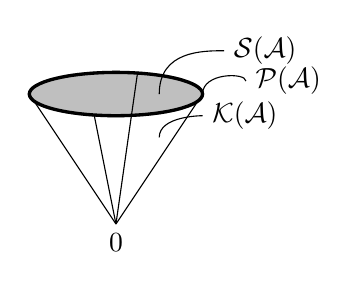
\begin{tikzpicture}[scale=0.55]
        \filldraw[gray!50,very thick] (0,3) ellipse (2 and 0.5);
        \draw[very thick] (0,3) ellipse (2 and 0.5);
        \draw (0,0) node[below] {$0$} --(-2,3);
        \draw (0,0) --(2,3);
        \draw (0,0) --(-0.5,2.5);
        \draw (0,0) --(0.5,3.5);
        \draw (1,3) .. controls (1,4) and (2,4) .. (2.5,4) node[right]{$\Ss(\As)$};
        \draw (2,3) .. controls (2,3.5) and (3,3.5) .. (3,3.3) node[right]{$\Ps(\As)$};
        \draw (1,2) .. controls (1,2.5) and (2,2.5) .. (2,2.5) node[right]{$\Ks(\As)$};
    \end{tikzpicture}
    \caption{ Sketch of the sets in the proposition.} 
    %\label{}
\end{figure}
\begin{proof}\leavevmode
    \begin{enumerate}[(1)]
        \item We set $E = \ex(\Ks(\As))$. 
        
    \ul{$0\in E$}. Assume $\psi_{1},\psi_2 \in \Ks(\As)$. $0 < t<1$. 
$0 = t\psi_1 + (1-t)\psi_2$. For $A \in \As$ we have 
$0\leq t \psi_1(A^*A) = \ub{(t-1)}_{< 0}\psi_{2}(A^*A) < 0$.
So we get that $\psi_1 (A^*A) =0$ for all $A \in \As$. It follows that $\psi_1 =0$,
which implies that $\psi_2 =0$.

\ul{$\Ps(\As)\subseteq E$}. 
Assume $\vphi \in \Ps(\As)$, $\vphi = t\psi_1 + (1-t)\psi_2$, $t \in (0,1)$,
$\psi_i \in \Ks(\As)$ for $i=1,2$.
Then $0\leq t\psi_1 \leq \vphi$ so $t\psi_1 \in K_{\vphi}$. Since $\vphi$
is pure, we must have $t \psi_1 = t'\vphi$ for some $t'\in [0,1]$.
Now since $\vphi \in \Ss(\As)$, which is a face of $\Ks(\As)$, we have 
$\psi_1 \in \Ss(\As)$ for $i=1,2$.
Hence we get $t= t \ub{||\psi_1||}_{=1} = ||t\psi_1|| = ||t'\vphi|| = t'$,
which implies that $\psi_1 =\vphi$ ($t\neq 0$), which in turn implies that 
$\psi_2 = \vphi$. Hence $\vphi \in E$.

\ul{$E \subseteq \{0\}\cup \Ps(\As)$}: Consider $\vphi \in E$, $\vphi \neq 0$.
Have to show that $\vphi \in \Ps(\As)$. If $||\vphi|| < 1$ then there is a 
$t \in (0,1)$ such that $\vphi = t
\ub{\(\tfrac{1}{t}\vphi\)}_{\in \Ks(\As)} + (1-t)\ub{0}_{\in\Ks(\As)}$.
This contradicts that $\vphi\in E$.

So 
$\vphi\in \Ss(\As)$ and moreover $\vphi$ is pure:
Indeed, let $\psi \in K_{\vphi}$, $0\neq \psi$, $\psi\neq \vphi$.
We can then write $\vphi = \psi +\ub{(\vphi -\psi)}_{\coloneqq \psi'}$
where $\psi, \psi'\geq 0$.
Set $t = ||\psi|| \in (0,1)$. We then get $1 =||\vphi|| = ||\psi|| + ||\psi'||=t +||\psi'||$,
so $||\psi'||=1-t$. So 
\[\vphi = t\ub{\(\tfrac{1}{t}\psi\)}_{\in\Ks(\As)} +
(1-t)\ub{\(\tfrac{1}{1-t}\psi'\)}_{\in\Ks(\As)}\]
Since $\vphi\in E$ we must have $\tfrac{1}{t}\psi = \vphi$. So $\psi = t\vphi$.
This shows that $K_{\vphi} = \{\la\vphi : 0\leq \la \leq 1\}$ as desired. 

\item Follows from $(1)$ since $\Ss(\As)$ is a face of $\Ks(\As)$ and $\Ps(\As)$
is a subset of $\Ss(\As)$.
\item[$(4)$ and $(3)$] Are consequences of Krein-Milman's theorem combined 
with $(1)$ and $(2)$.

\end{enumerate}
\end{proof}


\begin{proposition}
    Let $\vphi \in \Ss(\As)$, with GNS-triple $(\pivp, \Hvp, \xivp)$.
Set 
\[R_{\vphi} = \{ T \in \pivp(\As)' : ||T||\leq 1, T \geq 0 \}.\] 
Then there is a bijection $T \mapsto \psi_{T}$ from $R_{\vphi}$ onto
$K_{\vphi} = \{\psi \in \Ks(\As) : 0\leq \psi\leq \vphi\}$
(respecting convex combinations (affine map)) given by
\[ \psi_{T}(A) = \ind{\pivp(A)\xivp, T\xivp}\qquad\text{for all } A \in \As \]
and for each $T \in R_{\vphi}$.
\end{proposition}
\begin{proof}
    Let $T \in R_{\vphi}$ and define $\psi_T$ as above. Clearly $\psi_{T}$
is a linear functional on $\As$. $\psi_T \in K_{\vphi}$. 
Set $S = T^{1/2} \in R_{\vphi}$ (Argue for this, use $\As$ is $C^*$-algebra).
For each $A \in \As$, we have 
\begin{align*}
\psi_T(A^*A) &= \ind{\pivp(A^*A)\xivp, T\xivp} \\
    &= \ind{\pivp(A)\xivp, \pivp(A)T\xivp} \\
&\underset{T\in\text{commutant}}{=} \ind{\pivp(A)\xivp, T\pivp(A)\xivp}\\
&= \ind{S\pivp(A)\xivp, S\pivp(A)\xivp} \geq 0
\end{align*}
so $\psi_T \geq 0$.
We also get 
\begin{align*}
    \psi_T(A^*A) &\underset{C.S.}{\leq} ||\pivp(A)\xivp|| \,||T\pivp(A)\xivp|| \\
&\leq ||\pivp(A)\xivp|| \,||T|| \,||\pivp(A)\xivp|| \\
&\leq \ub{||T||}_{\leq 1} \,||\pivp(A)\xivp||^2 \leq \vphi(A^*A)\quad\text{for all }A\in\As.
\end{align*}
Hence $\psi_T\leq \vphi$.

\ul{The map $T\mapsto \psi_T$ is injective:}
Assume $\psi_{T_1} = \psi_{T_2}$ for $T_1,T_2 \in R_{\vphi}$. Then 
\[ \ind{\pivp(A)\xivp, T_1\xivp-T_2\xivp} = 0 \quad \forall A\in \As\]
i.e. $(T_1\xivp - T_2\xivp) \in (\pi(\As)\xivp)^{\perp} = [\pi(\As)]^{\perp} =
\Hvp^{\perp}=\{0\}$.
Hence $T_1\xivp = T_{2}\xivp$. 
Thus 
\begin{align*}
    T_1\pivp(\As)\xivp = \pivp(\As)T_1\xivp = \pivp (\As)T_2 \xivp = T_2\pivp(\As)\xivp
\end{align*}
By density of $\pivp(\As)\xivp$, we get that $T_1 = T_2$ on $H_{\vphi}$.

\ul{The map $T\mapsto \psi_{T}$ is surjective:}
Let $\psi \in K_{\vphi}$. Observe that $A,B \in \As$, we have 
\begin{align*}
    |\vphi(B^*A)|^2 \underset{C.S}{\leq} \psi(A^*A)\psi(B^*B)\leq \vphi(A^*A)\vphi(B^*B) 
= ||\pivp(A)\xivp||^2 ||\pivp(B)\xivp||^2 \quad (*)
\end{align*}
Set $H_0 = \pivp(\As)\xivp$. We can now define a bounded sesquilinear form 
$\ind{\cdot,\cdot}_{\psi} \colon H_0\times H_0 \to \C$ by 
$\ind{\pivp(A)\xivp, \pivp(B)\xivp}_{\psi}\coloneqq \psi(B^*A)$
 for $A,B \in \As$.
(Using $(*)$, it is an easy exercise to check that form is well-defined. Assume
$\pivp(A)\xivp = \pivp(A')\xivp$, then $\psi(B^*(A-A'))\leq
||\pivp(A-A')\xivp||^2||\cdots||^2\leq 0$).

The boundedness follows from $(*)$ since it says that 
$|\ind{\pivp(A)\xivp, \pivp(B)\xivp}_{\psi}|\leq ||\pivp(A)\xivp||\, ||\pivp(B)\xivp||$,
so its norm $\leq 1$.

By density of $H_0$ in $\Hvp$, we can extend this form to a sesquilinear form 
$\ind{\cdot,\cdot}_{\psi}$ on $\Hvp$ with norm $\leq 1$. 
By the Riesz-representation theorem for such forms (see notes last course),
we get that there exits a unique $T\in \Bs(H_{\vphi})$ with $||T||\leq 1$ 
such that $\ind{\eta,\eta'}_{\psi} = \ind{T\eta,\eta'}$ for all $\eta,\eta' \in
\Hvp$.

Since $\ind{T\eta,\eta}= \ind{\eta,\eta}_{\psi} \geq 0$ for all $\eta \in \Hvp$
we have $T\geq 0$.

\ul{It remains to check that $T \in \pivp(\As)'$:}
We first note that 
\begin{align*}
\psi(B^*A) & = \ind{\pivp(A)\xivp, \pivp(B)\xivp} = 
\ind{T\pivp(A)\xivp, \pivp(B)\xivp} \\
&\underset{T\geq 0}{=} \ind{\pivp(A)\xivp, T\pivp(B)\xivp}\quad \forall A,B\in \As.
\end{align*}
Let now $A,B,C \in \As$,
then 
\begin{align*}
    \ind{\pivp(A)\xivp, T\pivp(B)\pivp(C)\xivp} &= \ind{\pivp(A)\xivp, T\pivp(BC)\xivp}\\
&= \psi((BC)^*A) = \psi(C^*B^*A) \\
&= \ind{\pivp(B^*A)\xivp, T\pivp(C)\xivp}\\ 
&= \ind{\pivp(A)\xivp, \pivp(B)T\pivp(C)\xivp} 
\end{align*}
By density and continuity we get that 
\[ \ind{\eta, T\pivp(B)\eta'} = \ind{\eta,\pivp(B)T\eta'}\quad\forall \eta,\eta' \in \Hvp \]
This implies that $T \in \pivp(\As)'$.
All together we have shown that $T \in R_{\vphi}$.

Finally, let $\{e_{\al}\}$ be an approximate unit for $\As$. 
Then we get 
\begin{align*}
\psi(A) &= \lim_{\al} \psi(\ub{e_{\al}}_{=e_{\al}^{*}}A)
= \lim_{\al}\ind{T\pivp(A)\xivp, \pivp(e_{\al})\xivp} \\
&\underset{(**)}{=}
\ind{T\pivp(A)\xivp, \xivp} = \ind{\pivp(A)\xivp, T\xivp} = \psi_{T}(A)
\end{align*}
(where $(**)$ follows since $\pivp(e_{\al})\xivp \to \xivp$ since $\pivp$ is non-degenerate)
for all $A\in \As$. So $\psi=\psi_T$ as desired.  

\end{proof}

\begin{theorem}
    Let $\vphi \in \Ss(\As)$. Then $\pivp$ is irreducible 
$\iff$ $\vphi \in \Ps(\As)$.
\end{theorem}
\begin{proof}
    We have $\pivp$ irreducible 
\begin{align*}
    &\iff \pivp(\As)' = \C I_H \\
    &\iff R_{\vphi}= \{ tI_H : 0\leq t\leq 1 \}\\
    &\underset{\text{prev. prop.}}{\iff} K_{\vphi}=\{t\vphi : 0 \leq t \leq 1\}\\
&\iff \vphi \in \Ps(\As)
\end{align*}
\end{proof}

\begin{corollary}
$\pi \in \Rep(\As,H)$ be non-zero and cyclic with unit cyclic vector $\xi$. 
Let $\vphi \in \Ss(\As)$ be given by $\vphi(A) = \ind{\pi(A)\xi,\xi}$ for all 
$A\in\As$. Then $\pi$ is irreducible $\iff$ $\vphi \in \Ps(\As)$.    
\end{corollary}
\begin{proof}
    We have seen previously that $\pi\sim \pivp$, so it follows from the theorem. 
\end{proof}

\begin{theorem}[Hahn-Banach for pure states]
    Let $\Bs$ be a non-zero $C^*$-subalgebra of $\As$
and let $\rho \in \Ps(\Bs)$. Then there exists some $\vphi \in \Ps(\As)$
which extends $\rho$.
\end{theorem}
\begin{proof}
    Set $F = \{\psi \in \Ks(\As) : \psi\lvert_{\Bs} = \rho\}$. 
By the HB-result for states we know that $F\neq \emptyset$.
Moreover $F$ is weak$^*$-closed (agree in the limit) in $\ub{\Ks(\As)}_{\text{weak$^*$ comp.}}$
so $F$ is weak$^*$-compact. 

\ul{$F$ is a face of $\Ks(\As)$}:
Assume $\psi \in F$, $\psi = t \psi_1 + (1-t)\psi_2$, with $\psi_1,\psi_2\in \Ks(\As)$
and $t\in (0,1)$. 
Set $\rho_{i} = \psi_{i}\lvert_{\Bs}$ for $i=1,2$.
Then we have 
\[ \ub{\rho}_{\in \Ps(\Bs)} = t\ub{\rho_1}_{\in \Ks(\Bs)} + (1-t)\ub{\rho_{2}}_{\in \Ks(\Bs)} \]
since $\rho \in \ex(\Ks(\Bs))$ we get $\psi_{i}\lvert_{\Bs}=\rho_i = \rho$ for $i=1,2$,
i.e. $\psi_i \in F$ $i=1,2$ as desired.

By Krein-Milmans's theorem we get that $F$ has at least one extreme point, say
$\vphi\in F$. Then $\vphi$ is an extreme point of $\Ks(\As)$ i.e. by previous
proposition $\vphi\in \Ps(\As)$, since $\vphi\neq 0$ as desired.
\end{proof}

Before we write the next lemma, we recall the convention that if $\As$ is a $C^*$-algebra,
then 
\[\tAs = \begin{cases} \text{the unitization $\tAs$ of $\As$} &\text{if $\As$ is non-unital}\\
\As &\text{if $\As$ is unital} \end{cases} \]
\begin{lemma}
    Let $A \in \As$ be normal, $\la \in \Sp(A) = \Sp_{\tAs}(A)$. 
Then there exists $\tvphi \in \Ps(\tAs)$ such that $\tvphi (A) = \la$.
\end{lemma}
\begin{proof}
    Set $\Bs = C^*(A,I)$ (which is abelian). By Gelfand theory we can find
$\rho \in \widehat{\Bs}$ such that $\rho(A)= \la$.
But $\rho \in \Ps(\Bs)$, so we can extend it to $\Ps(\tAs)$ by the HB-theorem above. 
\end{proof}

\begin{theorem}[Gelfand-Raikow]
    Let $A\in \As$. Then there exits an \ul{irreducible} representation 
$\pi$ of $\As$ such that $||\pi(A)|| = ||A||$.
In particular if $A\neq B$, $A,B\in \As$, then we can find an 
irreducible representation $\pi$ such that $\pi(A)\neq \pi(B)$. 
\end{theorem}
\begin{proof}
    Apply the lemma to $A^*A$ (normal) and $\la \in \Sp(A^*A)$
satisfying $|\la|= ||A^*A||$, we get that there exits $\tvphi \in \Ps(\tAs)$
such that $|\tvphi(A^*A)| = |\la| = ||A||^2$. Note that $\pi_{\tvphi}$
is an irreducible representation of $\tAs$. Set 
$\pi \coloneqq \pi_{\tvphi}\lvert_{\As} \in \Rep(\As,H_{\tvphi})$.

$\pi$ is irreducible because 
$\pi(\As)' = (\pi(\As) + \C I)' = \pi_{\tvphi}(\tAs)' = \C I_{H_{\tvphi}}$
Finally 
\[ ||A||^2 = ||\tvphi(A^*A)|| = ||\pi_{\tvphi}(A)\xivp||^2 \leq ||\pi(A)||^2 \leq ||A||^2 \]
so $||\pi(A)|| = ||A||$. The last assertion follows from $A\neq B \implies A-B
\neq 0$, so $\pi(A-B)\neq 0$ i.e. $\pi(A)\neq \pi(B)$.

\end{proof}

\section{On irreducible representations and compact operators}

We let $H$ be a non-zero Hilbert space.

\begin{lemma}
    Let $\xi \in H$, $||\xi||=1$. We denote $P_{\xi}$ the orthogonal projection from 
$H$ onto $\Span{\xi}$. Then 
$P_{\xi}TP_{\xi} = \ind{T\xi,\xi}P_{\xi}$ for all $T \in \Bs(H)$. Operators of the form $P_{\xi}TP_{\xi}$ are usually called \emph{compressions}.
\end{lemma}
\begin{proof}
    Let $T \in \Bs(H)$ and $\eta \in H$. 
\begin{align*}
    (P_{\xi}TP_{\xi})(\eta) &= P_{\xi}T(\ind{\eta,\xi}\xi) = \ind{\eta,\xi}\ind{T\xi,\xi}\xi
= \ind{T\xi,\xi}P_{\xi}(\eta)
\end{align*}
\end{proof}
We have seen that $\Ks(H)$ is irreducible, in other words, the identity representation 
on $\Ks(H)$ on $H$ given by $\Id(T) = T$ for $T \in \Ks(H)$ is irreducible. In fact we have:

\begin{theorem}
    Assume $\pi$ is a non-zero irreducible representation of $\Ks(H)$ on some
Hilbert space $K$. Then $\pi$ is unitary equivalent to the $\Id$ representation
i.e.  there exist $U\colon H\to K$ such that $\pi(T) = UTU^*$ for all $T\in
\Ks(H)$.
\end{theorem}
\begin{proof}
    Since $\pi\neq 0$, so we can find $T\in \Ks(H)$, $T$ self-adjoint and such that 
$\pi(T)\neq 0$.

By the spectral theorem for compact self-adjoint operators, $T$ is diagonalizable 
with respect to some o.n.b $\{\xi_j\}_{j\in J}$ for $H$. Letting
$\{\la_{j}\}_{j\in J}$ denote the corresponding eigenvalues of $T$, we have seen that 
$\{\la_j\}_{j\in J} \subseteq C_{0}(J)$, and that $T = \sum_{j\in J}\la_j P_{\xi_j}$
(norm-convergent). Since $0\neq\pi(A) = \sum_{j\in J}\la_j \pi(P_{\xi_j})$
so we must have that there exits (at least one) $\xi \in H$, with $||\xi||=1$
such that $\pi(P_{\xi})\neq 0$. 

Choose now $\eta \in \pi(P_{\xi})(K)$, $||\eta||=1$. Consider $A \in \Ks(H)$. 
Then we have 
\begin{align*}
||\pi(A)\eta||^2 &= ||\pi(A)\pi(P_{\xi})\eta||^2    
=||\pi(AP_{\xi})\eta||^2 = \ind{\pi(AP_{\xi})\eta, \pi(AP_{\xi})\eta} \\
&= \ind{\pi(P_{\xi}A^*AP_{\xi})\eta, \eta}
\underset{\text{lemma}}{=} \ind{\ind{A^*A\xi,\xi}\pi(P_{\xi})\eta,\eta} \\
&= \ind{A^*A,\xi,\xi}\ind{\pi(P_{\xi})\eta,\eta} =\ind{A^*A,\xi,\xi}\ind{\eta,\eta}
= ||A\xi||^2   
\end{align*}
It follows that the map $U_0\colon \Ks(H)\xi \to \pi(\Ks(H))\eta$, $A\xi\mapsto \pi(A)\eta$
is well-defined and linear. Since $[\Ks(H)\xi] = H$ and $[\pi(\Ks(H))\eta] = K$ (since $\pi$ is irreducible), we can extend $U_0$ to a unitary $U\colon H\to K$. We then have $UA\xi = \pi(A)\eta$
for all $A \in \Ks(H)$. So for any $T \in \Ks(H)$ we set 
\[ [\pi(T)U](A\xi) = \pi(T)\pi(A)\eta = \pi(TA)\eta = UTA\xi \]
for all $A \in \Ks(H)$.
By density/continuity we get $\pi(T)U = UT$ i.e. 
$\pi(T) = UTU^*$ for all $T \in \Ks(H)$.
\end{proof}

Note: In particular, we get that $M_n(\C)$ has only one irreducible representation 
up to unitary equivalence. 


\begin{corollary}
    Let $\varphi \in \Ss(\Ks(H))$. Then $\vphi$ is pure $\iff$ $\vphi$ is a \emph{vector state}
on $\Ks(H)$ i.e. there exits $\xi \in H$, $||\xi||=1$ such that $\vphi(T) = \ind{T\xi,\xi}$
for all $T \in \Ks(H)$.
\end{corollary}
\begin{proof}
    Assume $\vphi$ is pure. Then we know that $\pi_{\vphi}$ is irreducible, so the 
theorem gives that there exits $U\colon H\to \Hvp$ unitary, such that 
$\pivp (T) = UTU^*$ for all $T \in \Ks(H)$.
Thus we have 
\begin{align*}
    \vphi(T) &= \ind{\pivp(T)\xivp, \xivp} = \ind{TU^*\xivp, U^*\xivp} = 
\ind{T\xi, \xi}
\end{align*}
where $\xi = U^*\xivp$, which is a unit vector in $H$, since $U^*$ is unitary
for all $T\in \Ks(H)$. 

Conversely, assume the RHS holds. Then we have 
\[ \vphi(T) = \ind{\Id(T)\xi,\xi}\quad\text{for all } T \in \Ks(H).\]
and $\xi$ is cyclic for $\Id$, since $\Id$ is irreducible we get from a
previous result that $\vphi$ is pure.
\end{proof}

\begin{corollary}
    Assume $\al\colon \Ks(H)\to \Ks(H')$ is a $*$-isomorphism. Then there exits 
$U\colon H\to H'$ unitary such that 
$\al(T) = UTU^*$ for all $T \in \Ks(H)$.
\end{corollary}
\begin{proof}
    $\al$ is a irreducible representation of $\Ks(H)$ on $H'$, the theorem applies. 
\end{proof}

Note that the same result is true for isomorphism from $\Bs(H)\to \Bs(H')$, 
but we shall not prove it. 

\begin{definition}
Let $\As$ be a $C^*$-algebra. Set $\Proj(\As) =\{P\in \As: P=P^*=P^2\}$.
We say that $P\in \Proj(\As)$ is \emph{minimal} in $\As$ when $P\neq 0$
and $Q \in \Proj(\As)$ with $0\neq Q \leq P \implies Q = P$.
\end{definition}

\begin{example}
    $P\in \Proj(\Bs(H))$ is minimal if $\Bs(H)$ $\iff$ $P$ has rank one.
\end{example}
\begin{example}
    Assume $P\in \Proj(\As)$, $P\neq 0$, $P\As P = \C P$. Then $P$ is minimal 
in $\As$: For if $Q \in \Proj(\As)$ and $0\neq Q\leq P$ then we have $PQP = Q =\la P$
for some $\la \in C$, since $Q\leq P \iff QP =Q \iff PQ =Q$ (elementary course exercise).
But $P$ is a projection $\iff$ $\la = 0$ or $\la =1$, but $Q\neq 0$, so $\la \neq 0$. This gives 
$Q = P$.
\end{example}

\begin{proposition}[Prop. 1]
    Assume $\Bs$ is a $C^*$-subalgebra of $\Ks(H)$, and we have $0\neq P\in \Proj(\Bs)$.
Then $P$ is minimal in $\Bs$ $\iff$ $PBP = \C P$.
\end{proposition}
\begin{proof}
    We have seen that $\impliedby$ holds in general. 
Assume $\implies$ holds i.e. that $P$ is minimal in $\Bs$.
Let $B\in \Bs$ be self-adjoint, $B\neq 0$. It suffices to show that $T\coloneqq PBP \in \C P$.
Note that $T$ is a compact self-adjoint operator in $\Bs$. Set $\La = \Sp(T)$.
Then we know that $\emptyset \neq \La \setminus \{0\}$ is isolated eigenvalues
of $T$. So we have $T = \sum_{\la \in \La\setminus\{0\}} \la P_{\la}$ where
$P_{\la} = \chi_{\{\la\}}(T) \in \Bs$ (which is continuous since $\{\la\}$ is
a isolated point). 

Set $M = P(H)$. Clearly $T = 0$ on $M^{\perp}$. Hence if $\eta \in M^{\perp}$, 
we get $0 = ||T\eta||^2 = \sum_{\la \in \La\setminus\{0\}} |\la|^2 ||P_{\la}\eta||^2$,
hence $P_{\la}\eta = 0$ for all $\la \in \La\setminus\{0\}$. 
Thus $P_{\la} (I-P)= 0 $ for all $\la \in \La\setminus\{0\}$
i.e. $P_{\la} = P_{\la}P$ for all $\la \in \La\setminus\{0\}$,
which holds if and only if $P_{\la}\leq P$ for all $\la \in \La\setminus\{0\}$.

Since $P$ is minimal in $\Bs$ we get $P_{\la} = P$ for all $\la \in \La\setminus\{0\}$,
but $P_{\la}\perp P_{\mu}$ for $\la \neq \mu$, so we must have that $\La
\setminus \{0\} = \{\la_1\}$, i.e. $T = \la_1 P$ as desired. 
\end{proof}

\begin{proposition}
    Assume $\Bs$ is a $C^*$-subalgebra of $\Ks(H)$, and $0\neq P\in \Proj(\Bs)$.
Then $P$ is a finite sum of minimal projections in $\Bs$.
\end{proposition}
\begin{proof}
    Since $Q \in \Proj(\Ks(H)) \implies Q$ has finite rank, it suffices to show that the
following assertion holds for any $n\in \N$. 

$A(n):$ Any element in $\Proj(\Bs)$ with rank between 1 and $n$ is a finite sum of 
minimal projections in $\Bs$ (which are orthogonal to each other).

\ul{$n=1$}: Trivial.

Assume $A(n-1)$ holds for some $n\geq 2$.
Let $E \in \Proj(\Bs)$ with $1\leq \rank(E)\leq n$.
If $E$ is minimal in $\Bs$ then OK. Otherwise, there exists some $F \in \Proj (\Bs)$
such that $0\neq F \leq E$, $F\neq E$. We can then write $E = F + \ub{E - F}_{F'}$.
Then $F' \in \Proj(\Bs)$, $F' \neq 0$ and $F'\leq E \neq F'$ and $FF' = 0$.
So we have $1\leq \rank(F)\leq n-1$ and $1\leq \rank(F') \leq n-1$.
Using that $A(n-1)$ holds, we get that $E$ is a sum of minimal projections in $\Bs$,
which are orthogonal to each other.
\end{proof}

\begin{theorem}
    Assume $\pi \in \Rep(\As,H)$ is non-zero, irreducible and $\pi(\As) \subseteq\Ks(H)$.
Then $\pi(\As) = \Ks(H)$.
\end{theorem}
Note that this can be used to show that if $\pi$ is irreducible and
$\pi(\As)\cap \Ks(H)\neq \{0\}$, then $\Ks(H)\subseteq \pi(\As)$.
\begin{proof}
    We set $\Bs = \pi(\As)$. So $\{0\}\neq \Bs \subseteq \Ks(H)$, $\Bs$ irreducible.
Want to show that $\Ks(H)\subseteq \Bs$. 

We first show that $\Bs$ contains a non-zero element.
Observe that $\Proj (\Bs)$ contains a non-zero element 
(we may consider a non-zero self-adjoint operator in $\Bs$ and pick one of its
spectral components). So using the previous proposition, we can find (at least)
one minimal projection in $\Bs$ say $P$. We claim that \ul{$P$ has rank one:}

Let $\xi \in P(H)$, $||\xi||=1$. Assume that $\eta \in P(H)$, $\eta\perp\xi$.
For all $B \in \Bs$ we get 
\begin{align*}
    \ind{B\xi,\eta} = \ind{BP\xi,P\eta} = \indi{PBP\xi,\eta} = \ind{\la P\xi, \eta} =
\la\ind{P\xi,\eta} = 0 
\end{align*}
where $PBP = \la P$ for some $\la \in \C$, since $P$ is minimal in $\Bs$.
Since $[\Bs \xi] = H$, we get $\eta \in [\Bs \xi]^{\perp} = H^{\perp} = \{0\}$ 
i.e. $\eta = 0$. Hence $P(H) = \Span{\xi}$ i.e. $P=P_{\xi}$ (cf. previous notation).  

\ul{Next $\Proj (\Bs)$ contains all the rank one projections:}
Let $\xi' \in H$, $||\xi'||=1$. As $[\Bs\xi] = H$, we can find $\{B_{n}\} \subseteq \Bs$
such that $B_n\xi \to \xi'$ in norm. Then $P_{\xi'} = \text{norm-}\lim_{n\to\infty}
B_{n}PB_{n}^{*} \in \Bs$.
Indeed, for all $\eta\in H$, we have
\begin{align*}
    ||(B_nPB_{n}^{*} - P_{\xi'})(\eta)|| 
&\leq ||B_n(\ind{B_{n}^*\eta,\xi}\xi) - \ind{\eta,\xi'}\xi'|| = 
||\ind{\eta,B_{n}\xi}B_n\xi - \ind{\eta,\xi'}\xi'|| \\
&\leq ||\ind{\eta,B_{n}\xi}B_n\xi -\ind{\eta,B_n\xi}\xi'|| 
+||\ind{\eta,B_n\xi}\xi'- \ind{\eta,\xi'}\xi'|| \\
&\leq |\ind{\eta, B_n\xi}|\,||B_n \xi- \xi'|| + |\ind{\eta,B_n\xi -\xi'}|\,\ub{||\xi'||}_{=1} \\
&\underset{C.S}{\leq} ||\eta|| \,||B_n\xi-\xi'|| (||B_n\xi|| + 1)
\end{align*}
So 
\begin{align*}
    ||B_nP B_{n}^{*}-P_{\xi'}|| 
    \leq \ub{||B_n\xi - \xi'||}_{\to 0} \ub{(||B_n\xi||+1)}_{\to 2}\to 0 
\end{align*}
It follows that $\Bs$ contains all compact self-adjoint operators. Hence all
compact operators. 
\end{proof}

\begin{theorem}
    Let $\As$ be a non-zero finite-dimensional $C^*$-algebra. Then $\As \simeq M_{n_1}(\C)\oplus 
\cdots \oplus M_{n_k}(\C)$ for $n_1,\ldots, n_k \in \N$.
\end{theorem}
\begin{proof}
    We first observe that any finite dim $C^*$-algebra $\As$ is unital. 
By Gelfand-Neinmark we can find $\pi \in \Rep(\As,H)$ which is faithfull and non-degenerate. 
Since $\pi(\As)$ is finite dim, it is closed in the SOT. Now let $\{e_{\al}\}$ be 
and approximate unit for $\As$. Then $\pi(e_{\al}) \to I_H$ in the SOT i.e.
$I_H \in \ol{\pi(\As)}^{SOT} = \pi(\As)$. Pick $e \in \As$, such that $\pi(e) = I_H$.
Then $e$ is easily seen to be unit for $\As$.

Next we observe that $\As$ contains (at least) one minimal ideal $\Js$: This
means that $\Js$ is an ideal of $\As$, which is non-zero and contains no other
ideals of $\As$, than $\{0\}$ and itself. Equivalently, $S$ is simple  as
$C^*$-algebra. 

Indeed, if $\As$ is simple then OK. Otherwise, we can find an ideal $\Js_1\neq\{0\}$,
$\Js_1 \neq \As$. Then $1\leq \dim \Js < \dim \As$. If $\Js_1$ is simple, then OK,
if not we can find as long as necessary, but only a finite number of times. We get an ideal $\Js$
which is simple. 

We have to show that $J \simeq M_{n}(\C)$, for some $n\in \N$. Let $\pi$
be a faithfull non-zero irreducible representation of $\Js$ on some $H$.
Then $\pi$ is faithfull (otherwise $\ker \pi$ would be an ideal in $\Js$, which is non-zero
and not equal to $\Js$).

Moreover, $H$ is finite dimensional, since $H = [\pi(\As)\xi]$, where $\As$ is finite dimensional,
for any $\xi \neq 0$.
So $\pi(\As)\subseteq \Bs(H) = \Ks(H)$
By the previous theorem, $\pi(\As) = \Ks(H) = \Bs(H)$, so $\As = \Bs(H) = M_n(\C)$, 
$n = \dim H$.

We have that $\As \simeq \Js +\Ls$ for some ideal $\Ls$ of $\As$.
Let $P$ denote the unit of $\Js$. Note that $AP =PA$ for all $A \in \As$,
because $PA=P\ub{PA}_{\in \Js} = P\ub{AP}_{\in \Js} = AP$
Set $\Ls = (E-P)\As$ (where $E$ is the unit in $\As$) (we say that $E-P$ lies
in the center of $\As$).
Then one checks that $\Ls$ is an ideal of $\As$, such that $\As = \Js + \Ls$ 
(because $A = PA + (E-P)A$) and $\Js\cap \Ls = \{0\}$.
If $C = PA = (E-P)B$, then $C = PAP = \ub{P(E-P)}_{=0}B = 0$. 
Then the map $(\Js,\Ls)\to \Js + \Ls$ is a $*$-isomorphism for $\Js \oplus \Ls$ 
onto $\As$. 
We can now continue with $\Ls$ if necessary. Doing this (a finite number of times)
gives the result.


\end{proof}



















\end{document}




